En este capitulo se describen los principales aspectos de la solución al problema
de la exploración multi-robot desarrollada en este proyecto\footnote{Disponible
en línea:\\
\url{https://gitlab.fing.edu.uy/federico.ciuffardi/pgmappingcooperativo}},
incluyendo las potenciales mejoras que constituyen las contribuciones del
proyecto de grado (sección \ref{sec:cont}).

El capitulo comienza con la sección \ref{sec:hip} donde se enumeran las
hipótesis de trabajo. Luego en la sección \ref{sec:arqui} se describe la
arquitectura de la solución. Seguido de esto, en la sección \ref{sec:def} se
detallan y formalizan conceptos que son fundamentales en la solución propuesta.

Lo que resta del capitulo se dedica a profundizar en diversos aspectos de la
solución. A continuación se destacan las secciones donde se tratan las
contribuciones del proyecto. En la sección \ref{subsec:MiSimp} se describe el
método de simplificación de fronteras propuesto. En la sección
\ref{subsec:MiResSub} se introduce el algoritmo de asignación de objetivos. La sección
\ref{subsec:mapaTopGVDGrid} se comenta como el algoritmo de
construcción incremental del GVD y la forma novedosa de tratar
las porciones desconocidas del espacio durante la construcción del GVD.
Finalmente la sección \ref{sec:miNav} se describe la planificación jerárquica
propuesta.

% En la sección \ref{sec:hip} se establecen las hipótesis asumidas para el
% desarrollo de la solución. En la sección \ref{sec:arqui} se describe al
% arquitectura de la solución. En la 
% Para el problema de asignación de objetivos (sección \ref{sec:exploracion}) se
% presentan soluciones para cada una de sus partes. Para la identificación de
% objetivos se propone una técnica novedosa basada en el rango de sensado de los
% robots que determina como objetivos a un subconjunto de los puntos fronterizos.
% La distribución de objetivos a robots, se resuelve de forma coordinada
% aplicando una variante de lo presentado en la sección \ref{subsec:wurmCoord}.

% La asignación requiere de la construcción de un mapa topológico, para esto se
% implementa la técnica descrita en la sección \ref{subsec:mapaTopGVD} que
% requiere de un GVD, el cual se construye de forma incremental con una variante
% del algoritmo \emph{brushfire dinámico} (sección \ref{subsec:constGVDInc}).

% Luego de asignado a un objetivo el robot deberá llegar hasta el, para esto es
% necesario solucionar el problema de planificación. La solución desarrollada
% aplica la idea de planificación jerárquica mencionada en la sección
% \ref{subsec:mapas}, con el motivo de permitir una planificación
% computacionalmente eficiente sin resultar en caminos innecesariamente largos.

% El problema construir el mapa de un entorno inicialmente desconocido a partir
% de los datos sensoriales de varios robots se soluciona, construyendo en cada
% robot, según la información sensorial que estos recolectan, una grilla de
% ocupación con el nodo de \gls{ROS} \emph{costmap\_2d} \cite{ROS-costmap_2d} y luego
% combinando dichas grillas con las ideas presentadas en
% \cite{stachniss2009robotic}.

\section{Hipótesis de trabajo}\label{sec:hip}
La solución se desarrolla con las siguientes hipótesis de trabajo.
\begin{enumerate}[label=(\roman*)]
  \item Cada robot puede obtener en todo momento su ubicación (posición y
    orientación) sin errores.
  \item Las comunicaciones son ideales: sin perdida, con un ancho de banda y rango infinito.
  \item Los robots son iguales entre sí.
  \item Los robots tienen la capacidad de detectar las superficies más cercanas
    que se encuentran dentro de un circulo de radio $rango$ centrado en el
    robot.
  \item El entorno a explorar es cerrado.
  \item Se conocen las dimensiones del entorno a explorar.
\end{enumerate}

Estas hipótesis tienen el motivo de simplificar algunos aspectos del
problema de exploración permitiendo que el trabajo se pueda enfocar en otros.

La hipótesis (I) resuelve trivialmente el problema de localización \cite{slam}. 

Las hipótesis (II) y (III) simplifican la coordinación. La (II) por no tener
que hacer consideraciones especiales para cada robot. La (III) por no tener que
considerarse los posibles problemas de comunicación que pueden haber de asignar
robots a objetivos muy distantes o con obstrucciones entre sí. 

La hipótesis (IV) establece la capacidad sensorial del robot. Que sea posible 
sensar un circulo centrado en el robot, evita considerar su orientación.

La hipótesis (V) es útil para poder aplicar el criterio de parada que consiste
en detener la exploración al no tener más objetivos restantes (sección
\ref{sec:exploracion}). 

Finalmente la hipótesis (VI) permite establecer una grilla de ocupación con las
dimensiones suficientes para representar todo el entorno a explorar. 

\section{Arquitectura}\label{sec:arqui}
La arquitectura se divide en dos tipos de componentes robots y unidad central.
Existe una única unidad central que se encarga de centralizar la información
del entorno explorado y de coordinar a los varios robots que pueden existir.
Cada componente esta asociado a un hardware específico, siendo los robots móviles
y la estación central estática. 
%Los robots pueden ser uno o más mientras que la estación central es única. 
Los componentes a su vez se componen de módulos los cuales cuales se encargan
de tareas específicas. 

En la figura \ref{fig:arquitectura} se resume la arquitectura en un diagrama en
el cual es posible ver los componentes, sus módulos y como estos se distribuyen
sobre los componentes. Adicionalmente es posible apreciar una simplificación de las
comunicaciones que ocurren entre dichos módulos.


\begin{figure}[H]
  \center
  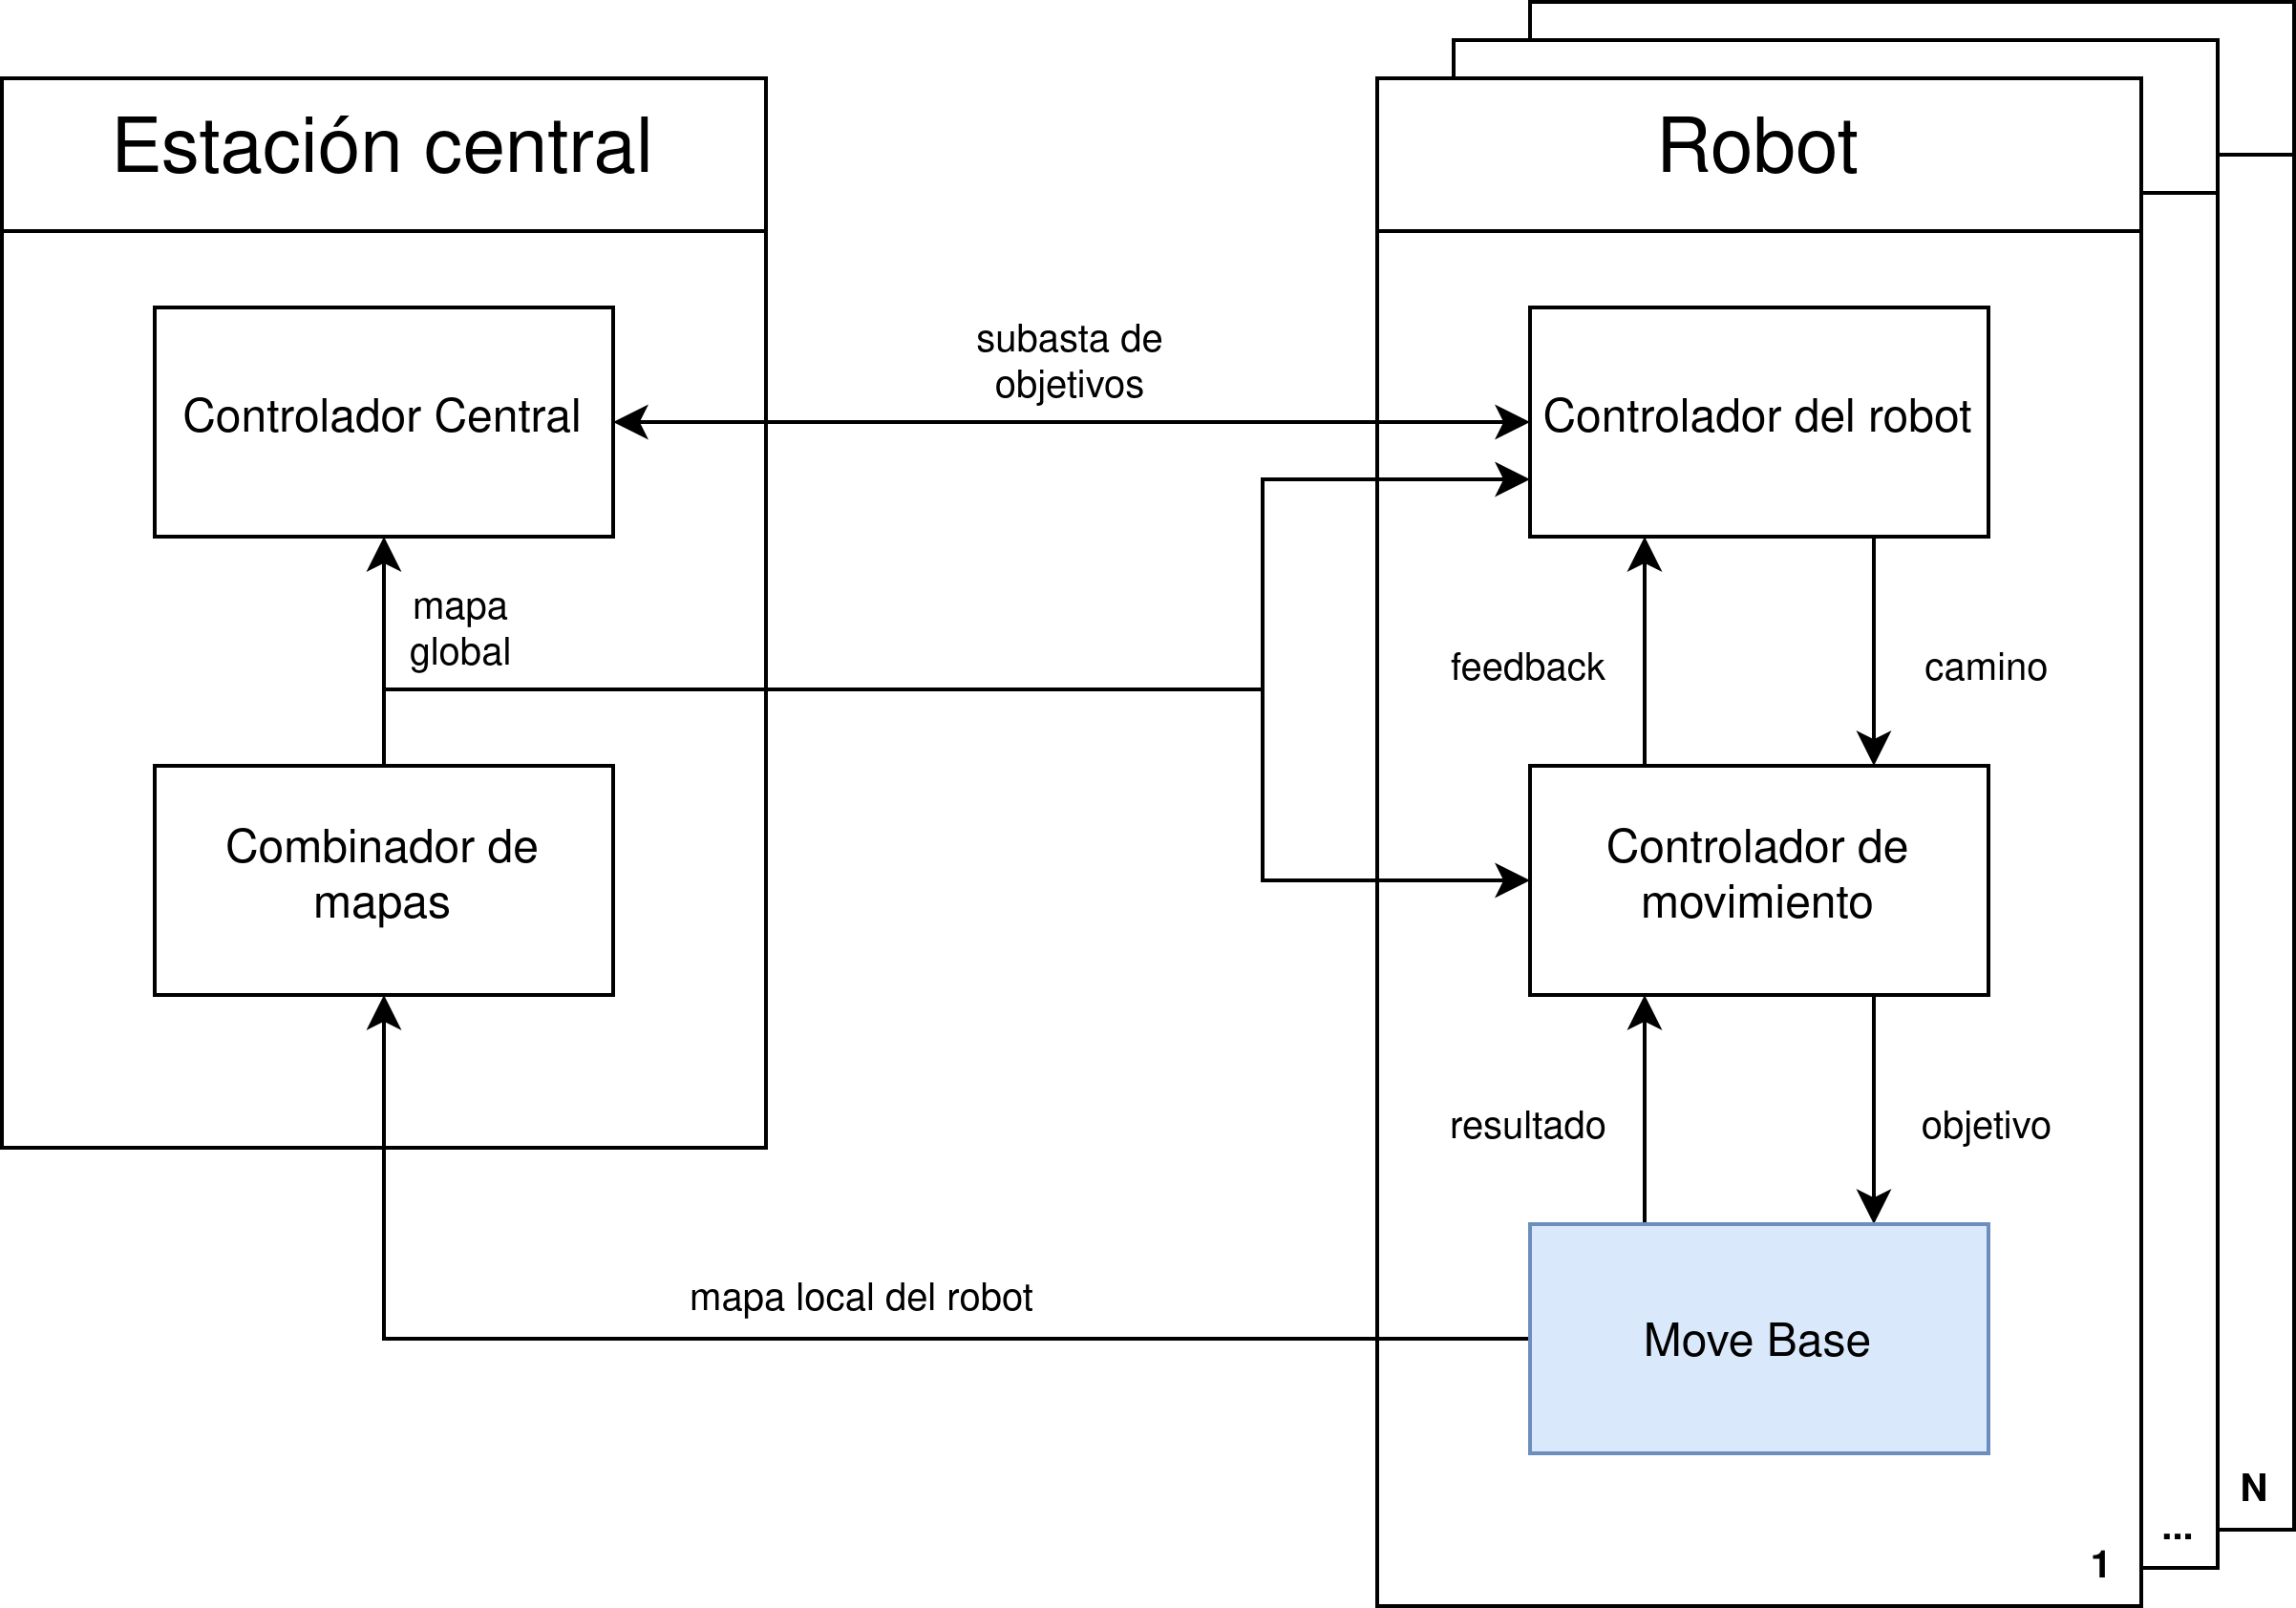
\includegraphics[width=1\linewidth]{imagenes/arquitectura.png}
  \caption[Arquitectura de la solucion propuesta.]{Arquitectura de la solución propuesta. Los módulos no coloreados fueron implementados en esta propuesta.}
  \label{fig:arquitectura}
\end{figure} 

En lo que resta de esta sección se comentará de cada modulo tanto sus tareas,
como sus interacciones con el resto de los módulos.

\subsection{Move Base}\label{subsec:move_base}
El modulo \emph{Move Base} consiste en una instancia del nodo \gls{ROS}
\emph{move\_base} \cite{ROS-move_base} que provee una interfaz para configurar,
ejecutar y interactuar con el \emph{stack de navegación} de \gls{ROS}
\cite{ROS-navigation}. 

El stack de navegación de \gls{ROS} es un conjunto de nodos que tienen como propósito
que un robot pueda navegar el entorno hacia objetivos dentro del mismo. En la
figura \ref{fig:move_base} se muestra un diagrama que representa a los nodos que
componen al stack de navegación de \gls{ROS} y sus interacciones.

\begin{figure}[H]
  \center
  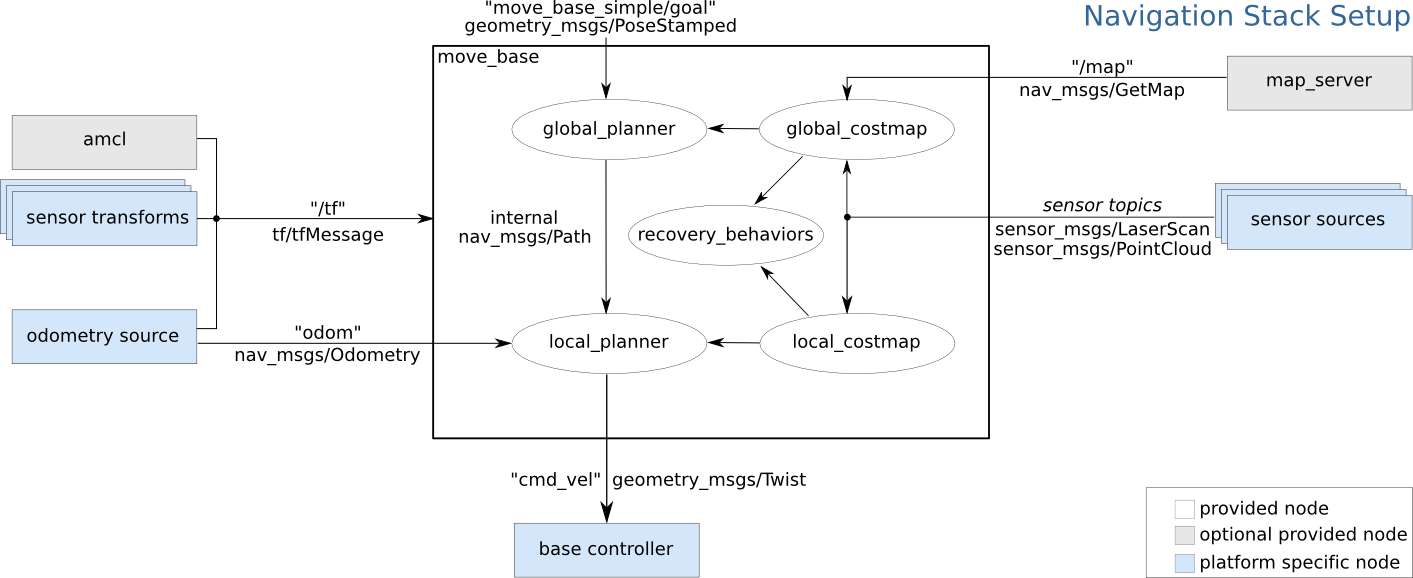
\includegraphics[width=1\linewidth]{imagenes/move_base.png}
  \caption[Arquitectura del stack de navegación de ROS.]{Arquitectura del stack de navegación de \gls{ROS}. Extraída de \cite{ROS-move_base}.}
  \label{fig:move_base}
\end{figure} 

Cuando se establece un objetivo de navegación este se trasmite al nodo
\emph{global\_planner} este se encarga de generar un plan de alto nivel
consistente de un numero de subobjetivos, que de seguirse en secuencia llevan
al robot al objetivo sin colisiones.

El camino generado por el \emph{global\_planner} es enviado al nodo
\emph{local\_planner} que se encarga de tomar el plan en alto nivel y
traducirlo a la secuencia las velocidades lineales y angulares que un robot
debe tener a lo largo del tiempo para seguir el global. A dicha secuencia de
velocidades se le conoce como plan local.

El stack de navegación permite utilizar distintas implementaciones de
\emph{global\_planner} y \emph{local\_planner}. En el trabajo desarrollado se
hace uso del \emph{global\_planner}\cite{ROS-global_planner} valga la
redundancia llamado \emph{global\_planner} y el \emph{local\_planner} llamado
\emph{teb\_local\_planner}\cite{ROS-teb_local_planner}.

Para generar sus planes tanto \emph{local\_planner} como \emph{global\_planner}
requieren de un mapa, de esto se encargan los nodos \emph{local\_costmap} (mapa
local) y \emph{global\_costmap} (mapa global) respectivamente. Ambos dos son
una instancia de una misma clase de nodo llamada \emph{costmap\_2d}
\cite{ROS-costmap_2d}, que dentro de sus funcionalidades esta la de de
construir una grilla de ocupación a partir de los datos sensoriales provistos
por los robots. Las principales diferencias entre el mapa global y el local son su
tamaño de celda (pequeño en el local y grande en el global), sus dimensiones
del mapa (el mapa global es el mapa completo mientras que el local es solo una
porción) y sus marcos de referencia (el mapa global suele estar fijo, el local se
centra en el robot).

El nodo \emph{recovery\_behaviors} permite ejecutar comportamientos de
recuperación de detectarse que el robot no esta avanzando de forma correcta al
objetivo. Para la solución desarrollada solo se hace uso del comportamientos de
recuperación que consiste en que el robot rote en el lugar.

\subsection{Combinador de mapas}
El modulo \emph{Combinador de mapas} es el encargado de mantener el mapa del entorno
explorado. Este recibe las actualizaciones de los mapas globales que son
generados por el nodo \emph{global\_costmap} del stack de navegación de cada
robot y las combina en un único mapa que contenga toda la información
recopilada del entorno. Cuando el mapa combinado global se actualiza este
retransmite lo actualizado a diversos componentes del sistema (ver figura
\ref{fig:arquitectura}) que utilizan el mapa del entorno explorado para llevar a
cabo alguna de sus tareas. 

\subsection{Controlador central}

El modulo \emph{Controlador central} es el responsable de orquestar la
asignación de objetivos. Específicamente la asignación de objetivos consiste en
una subasta en la cual este modulo actúa como subastador. La subasta se puede
resumir de la siguiente manera, los objetivos de exploración identificados son
transmitidos desde el \emph{controlador central} a los robots los cuales valúan
a dichos objetivos según que tan conveniente les es llegar a ellos. Los robots
envían sus valuaciones a la central la cual aplica una algoritmo para determinar
que objetivo le corresponde a cada robot y posteriormente le informa a cada
robot que objetivo le corresponde.

\subsection{Controlador de movimiento}
El modulo \emph{Controlador de movimiento} es como su nombre lo indica el modulo
que se encarga de controlar el movimiento del robot. Específicamente recibe
caminos compuesto por celdas de la grilla de ocupación que en secuencia llevan
a un objetivo de exploración, y se encarga de ir enviando objetivos de
navegación al modulo \emph{Move Base} para que el camino sea ejecutado de forma
rápida evitando maniobras innecesarias.

También lleva a cabo una capa superior de comportamientos de recuperación
extendiendo los provistos por el modulo \emph{Move Base}.

Indica al \emph{Controlador del robot} si se completo el camino con éxito, o
existe algún problema.

\subsection{Controlador del robot}
El \emph{Controlador del robot} es el modulo que se encarga de valuar los
objetivos cuando ocurre una subasta. A su vez se encarga de procesar los
objetivos asignados determinando el camino que lleva al objetivo y
enviándolo al modulo \emph{Controlador de movimiento}. 

También es responsable por solicitar el inicio de una subasta al
\emph{Controlado central} cuando el \emph{Controlador de movimiento} indica el
éxito o el fracaso en seguir el camino asignado.

\section{Definiciones} \label{sec:def}
Esta sección esta dedicada a formalizar conceptos que serán utilizados en lo que resta
del capitulo.

\subsection{Grillas de ocupación}\label{subsec:Grilla}
En el contexto de este trabajo se utilizará las siguientes definiciones referentes a
grillas de ocupación, introducidas en la sección \ref{subsec:mapas}.

El conjunto $\mli{CG}\subseteq R^2$ esta conformado de los centros de cada celda de la
grilla de ocupación. Las celdas se representan según sus centros y viceversa
sin ambigüedad, por lo tanto en lo que resta de este informe se usaran ambos
términos de forma indistinta.

Se dice que cada celda $c\in \mli{CG}$ tiene asociada una probabilidad $P(c|x_{1:t},z_{1:t})$
de estar ocupada, donde $z_{1:t}$ es la secuencia de medidas obtenidas de los
sensores desde las posiciones $x_{1:t}$.

La función $e : \mli{CG} \rightarrow E$ dado un centro de celda, devuelve uno de los
tres estados posibles $E=\{libre, ocupado, desconocido\}$ según la probabilidad
asociada a $c$. En el contexto de este proyecto la función $e$ se define según
(\ref{eq:estado}).
\begin{equation} 
  e(c)= 
  \left \{ 
    \begin{aligned}
       libre       &\ \ \ \text{ si}& P(c|x_{1:t},z_{1:t}) < 0.5 \\
       desconocido &\ \ \ \text{ si}& P(c|x_{1:t},z_{1:t}) = 0.5 \\
       ocupado     &\ \ \ \text{ si}& P(c|x_{1:t},z_{1:t}) > 0.5
    \end{aligned}
  \right .
  \label{eq:estado}
\end{equation}

La función $ady_4 : \mli{CG} \rightarrow P(\mli{CG})$ dada una celda $c$ devuelve el conjunto
de celdas horizontalmente adyacentes y la función $ady_8 : \mli{CG} \rightarrow P(\mli{CG})$
devuelve el conjunto de celdas adyacentes horizontal y diagonalmente. Las
definiciones de $ady_4$ y $ady_8$ se presentan en (\ref{eq:vecinos4}) y
(\ref{eq:vecinos8}) respectivamente donde $n_2, n_4, n_6, n_8$ se corresponden
a vecinos horizontales y $n_1, n_3, n_5, n_7$ se corresponden a los vecinos
diagonales de $c$ según se muestran en la figura \ref{fig:vecinos}.

\begin{equation} 
 ady_4(c)=\{n_{i*2} : 1\leq i \leq 4, n_{i*2} \in C\}
 \label{eq:vecinos4}
\end{equation} 

\begin{equation} 
 ady_8(c)=\{n_i : 1\leq i \leq 8, n_i \in C\}
 \label{eq:vecinos8}
\end{equation} 

\begin{figure}[H]
  \center
  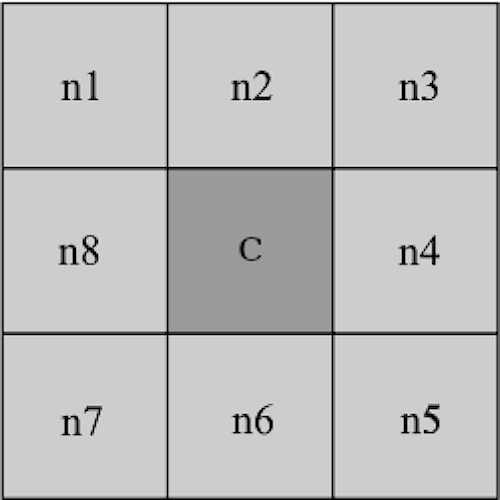
\includegraphics[width=0.3\linewidth]{imagenes/vecinosSharp.png}
  \caption[Vecinos de una celda en una grilla de ocupación.]{Vecinos de una celda en una grilla de ocupación.}
  \label{fig:vecinos}
\end{figure} 

Desde este punto se utilizará la función $ady$ como una función de adyacencia
genérica que puede ser tanto $ady_4$ como $ady_8$ a no ser que se indique lo
contrario.
Notar que la relación de adyacencia es simétrica por lo que $c_1 \in ady(c_2)
\Leftrightarrow c_2 \in ady(c_1)$.
% This map is obtained from the occupancy probability grid by a simple clipping operation with a threshold of 0.5. The gray areas of the maximum-likelihood map correspond to cells that have not been sensed by the robot.

\subsection{Componentes conexas} \label{subsec:CompComp}
Una descomposición en componentes conexas de un conjunto de
celdas $C \subseteq \mli{CG}$ es un conjunto $CC\in P(C)$ compuesto por $N$ conjuntos $C_i$ con
$i\in[1,N]$ tales que:
\begin{itemize}
  \item $\bigcup_{i=1}^{N}C_i = C$ 
  \item Para todo $i,j \in [1,N]$ $C_i\cap C_j = \emptyset$
  \item Para todo $i \in [1,N]$, para todo par $c_1,c_2 \in C_i$ se cumple que existe un camino de celdas adyacentes en $C_i$ que llevan desde $c_1$ a $c_2$.
  \item No existen $i,j \in [1,N]$ tales que existan $c_1 \in C_i$ y $c_2 \in C_j$ que cumplan con $c_1 \in ady(c_2)$ 
\end{itemize}

Un ejemplo de una descomposición en componentes conexas se muestra en la figura \ref{fig:fronterasCompCon}.

\begin{figure}[H]
  \centering
  \subfloat[Las celdas pertenecientes a $C$ se marcan con azul.]{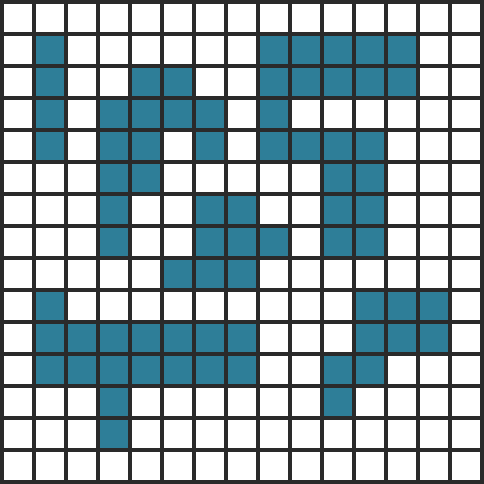
\includegraphics[clip=true, width=0.40\linewidth]{imagenes/compCon/a.png}}
  \qquad
  \subfloat[Cada componente conexa de $C$ se contornea con rojo.]{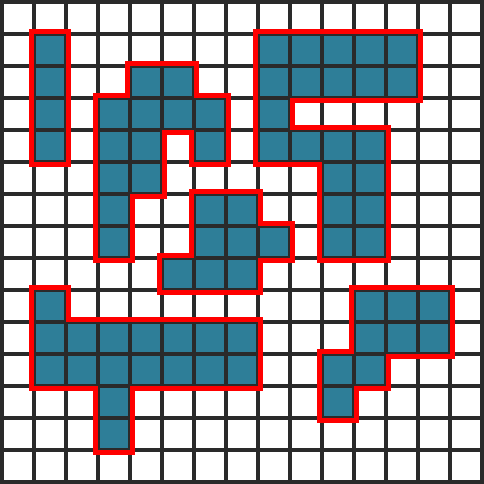
\includegraphics[clip=true, width=0.40\linewidth]{imagenes/compCon/b2.png}}

  \caption{Descomposición en componentes conexas.}\label{fig:descCompCon}
\end{figure}

Es posible obtener las componentes conexas de un conjunto cualquiera de
celdas $C$ con el algoritmo \ref{alg:compcon}.

\begin{algorithm}[H]
\SetAlgoLined
  \SetKwInOut{Input}{Entrada}
  \Input{$C$}
  $restantes := C$ \\
  $CC := \emptyset$ \\
  $pila :=$ Pila vacía \\
  $i := 1$ \\
  \While{ $\neg restantes.vacia()$ } {
    $C_i := \emptyset $ \\
    $c :=$ elemento arbitrario de $Restantes$ \\

    % \tcp{DFS desde $c$ agregando las celdas visitadas a la componente conexa $C_i$}

    $C_i :=  C_i \cup \{c\}$ \\
    $restantes := restantes - \{c\}$ \\
    $pila.apilar(c)$ \\
    \While { $\neg pila.vacia()$ } {
      $c := pila.desapilar()$ \\
      \ForEach{ $cA \in ady(c)$ } {
        \If{ $cA \in restantes$ } {
          $C_i :=  C_i \cup \{c\}$ \\
          $restantes := restantes - \{c\}$ \\
          $pila.apilar(c)$ \\
        }
      }
    }
    $CC := CC \cup C_i$ \\
    $i := i + 1$ \\
  }
  \Return $CC$ 

  \caption{Descomposición en componentes conexas de $C$}
  \label{alg:compcon}
\end{algorithm}

Este algoritmo se resume en elegir una celda $c\in C$ que no este aun en una
componente conexa (línea 6), aplicar un \emph{depth-first search} (DFS)
partiendo $c$ agregado todas las celdas recorridas a una misma componente
conexa (líneas 7-19). Repetir dicho procedimiento hasta que todas las celdas
pertenezcan a alguna componente conexa (línea 4). Este algoritmo es análogo al
que esta presente en \cite{hopcroft1973algorithm}.

\section{Identificación de objetivos}\label{sec:pc:idobj}
El problema de identificación de objetivos consiste en determinar los puntos
del espacio a los cuales es conveniente enviar robots para recolectar nueva
información sobre el entorno explorado. Estos puntos son los llamados objetivos
de exploración (sección \ref{sec:exploracion}). 

\subsection{Fronteras}
En \cite{yamauchi1998frontier} se propone que los lugares que permiten
recolectar la mayor cantidad de nueva información sobre el entorno son las
fronteras entre el espacio conocido y desconocido. Y que por lo tanto dichas
fronteras deben ser los objetivos de exploración.
Al utilizar una grilla de ocupación como mapa, las fronteras se definen como las
celdas cuyo estado asociado es $libre$ y son adyacentes a una celda cuyo estado
asociado es $desconocido$ (figura \ref{fig:fronteras}).
Por lo tanto según Yamauchi los objetivos de exploración serán las celdas
fronteras $F$ según se definen en (\ref{eq:fronteras}).
\begin{equation} 
  F = \{ c \in \mli{CG} : e(c) = libre, \exists n \in ady(c), e(n) = desconocido  \}
  \label{eq:fronteras}
\end{equation}

\subsection{simplificación de Fronteras basada en K-Means}
En \cite{Amorin2019} se argumenta que tratar todas las celdas fronteras
como objetivos de exploración diferentes podría ser computacionalmente
prohibitivo. Por lo tanto, para reducir el costo computacional, se intenta
reducir los objetivos de exploración a las celdas frontera más representativas,
a las cuales se denominaran como fronteras significativas.

Para determinar las fronteras significativas, primero, las celdas fronteras $F$
se descomponen en sus componentes conexas $\mli{FC}=\{F_1,F_2,...F_N\}$
(sección \ref{subsec:CompComp}), un ejemplo de este tipo de descomposición se
puede ver en la figura \ref{fig:fronterasCompCon}.

Luego se determinan las fronteras significativas $\mli{FS}_i$ de cada
componente conexa $F_i\in \mli{FC}$. Esto se hace agrupando las fronteras de
$F_i$ con el algoritmo K-Means \cite{macqueen1967some}, y determinando una
frontera significativa por cada una de las $k$ agrupaciones, la
frontera más cercana de $F_i$ al centroide de la agrupación (una arbitraria de
las más cercanas en el caso de que exista más de una). Un ejemplo de las
fronteras significativas  $\mli{FS} = \bigcup_{i=1}^N \mli{FS_i}$ obtenidas con
este método se muestra en la figura \ref{fig:fronterasSig}.

El $k$ utilizado para ejecutar K-Means es el mínimo que logra que para toda
frontera $f\in F_i$ existe $\mli{fs} \in FS_i$ tal que $d_{\mli{fs}}(f) \leq
rango$ siendo $rango$ el alcance de los sensores del robot. Es decir, el
conjunto de fronteras significativas $\mli{FS}_i \subset F_i$ cumple con que
cada frontera esta dentro del rango del sensado de alguna frontera
significativa, cuando esto se cumple se dice que $\mli{FS}_i$ cubre a $F_i$, o
que $FS_i$ logra el cubrimiento. En la figura \ref{fig:fronterasSigCub} se
puede ver como las fronteras significativas obtenidas $FS$ logran el
cubrimiento, ya que todas los centros de las fronteras $F$ están contenidos en
las circunferencias de radio $rango$ centradas en las fronteras significativas
$FS$.

Para encontrar el mínimo $k$ con las que se logra un $\mli{FS}_i$ que cubra a
$F_i$, se parte con $k=1$, si el resultado no logra cubrir incrementa $k$ y se
repite el proceso.


\begin{figure}[H]
  \centering
  \subfloat[Se identifican las frotneras,  marcadas con amarillo.]{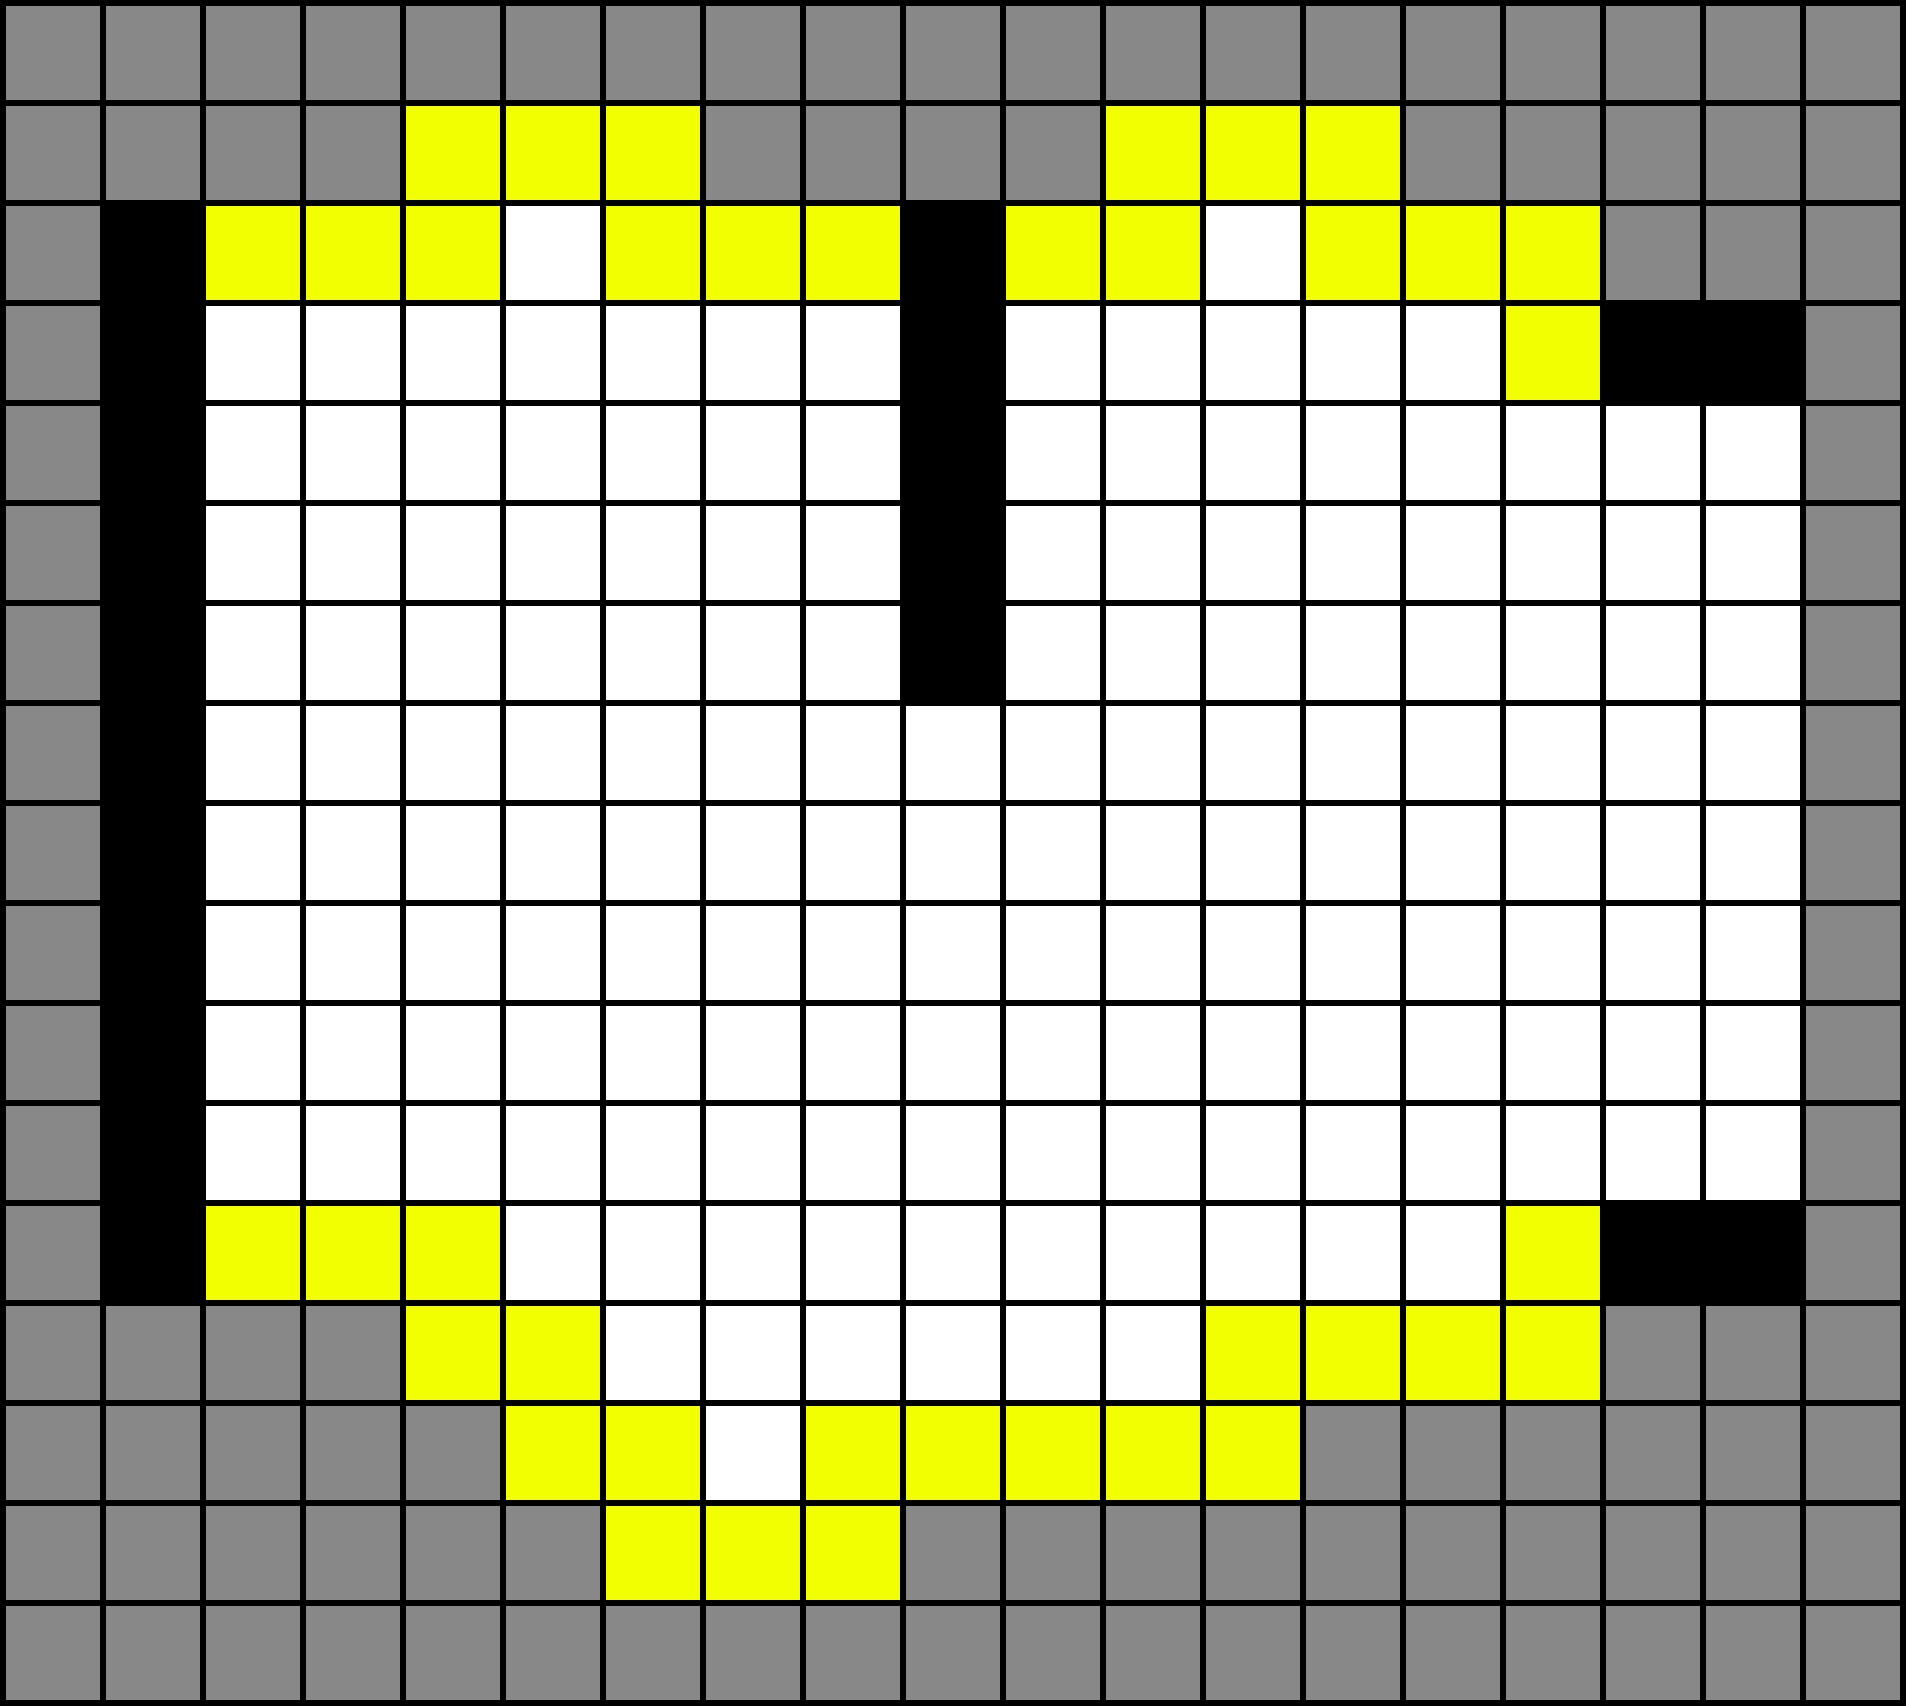
\includegraphics[clip=true, width=0.40\linewidth]{imagenes/fronterasSig/a.png}\label{fig:fronteras}}
  \qquad
  \subfloat[Descompocicion de las fronteras en componentes conexas, cada componente conexa se indica con un color distinto.]{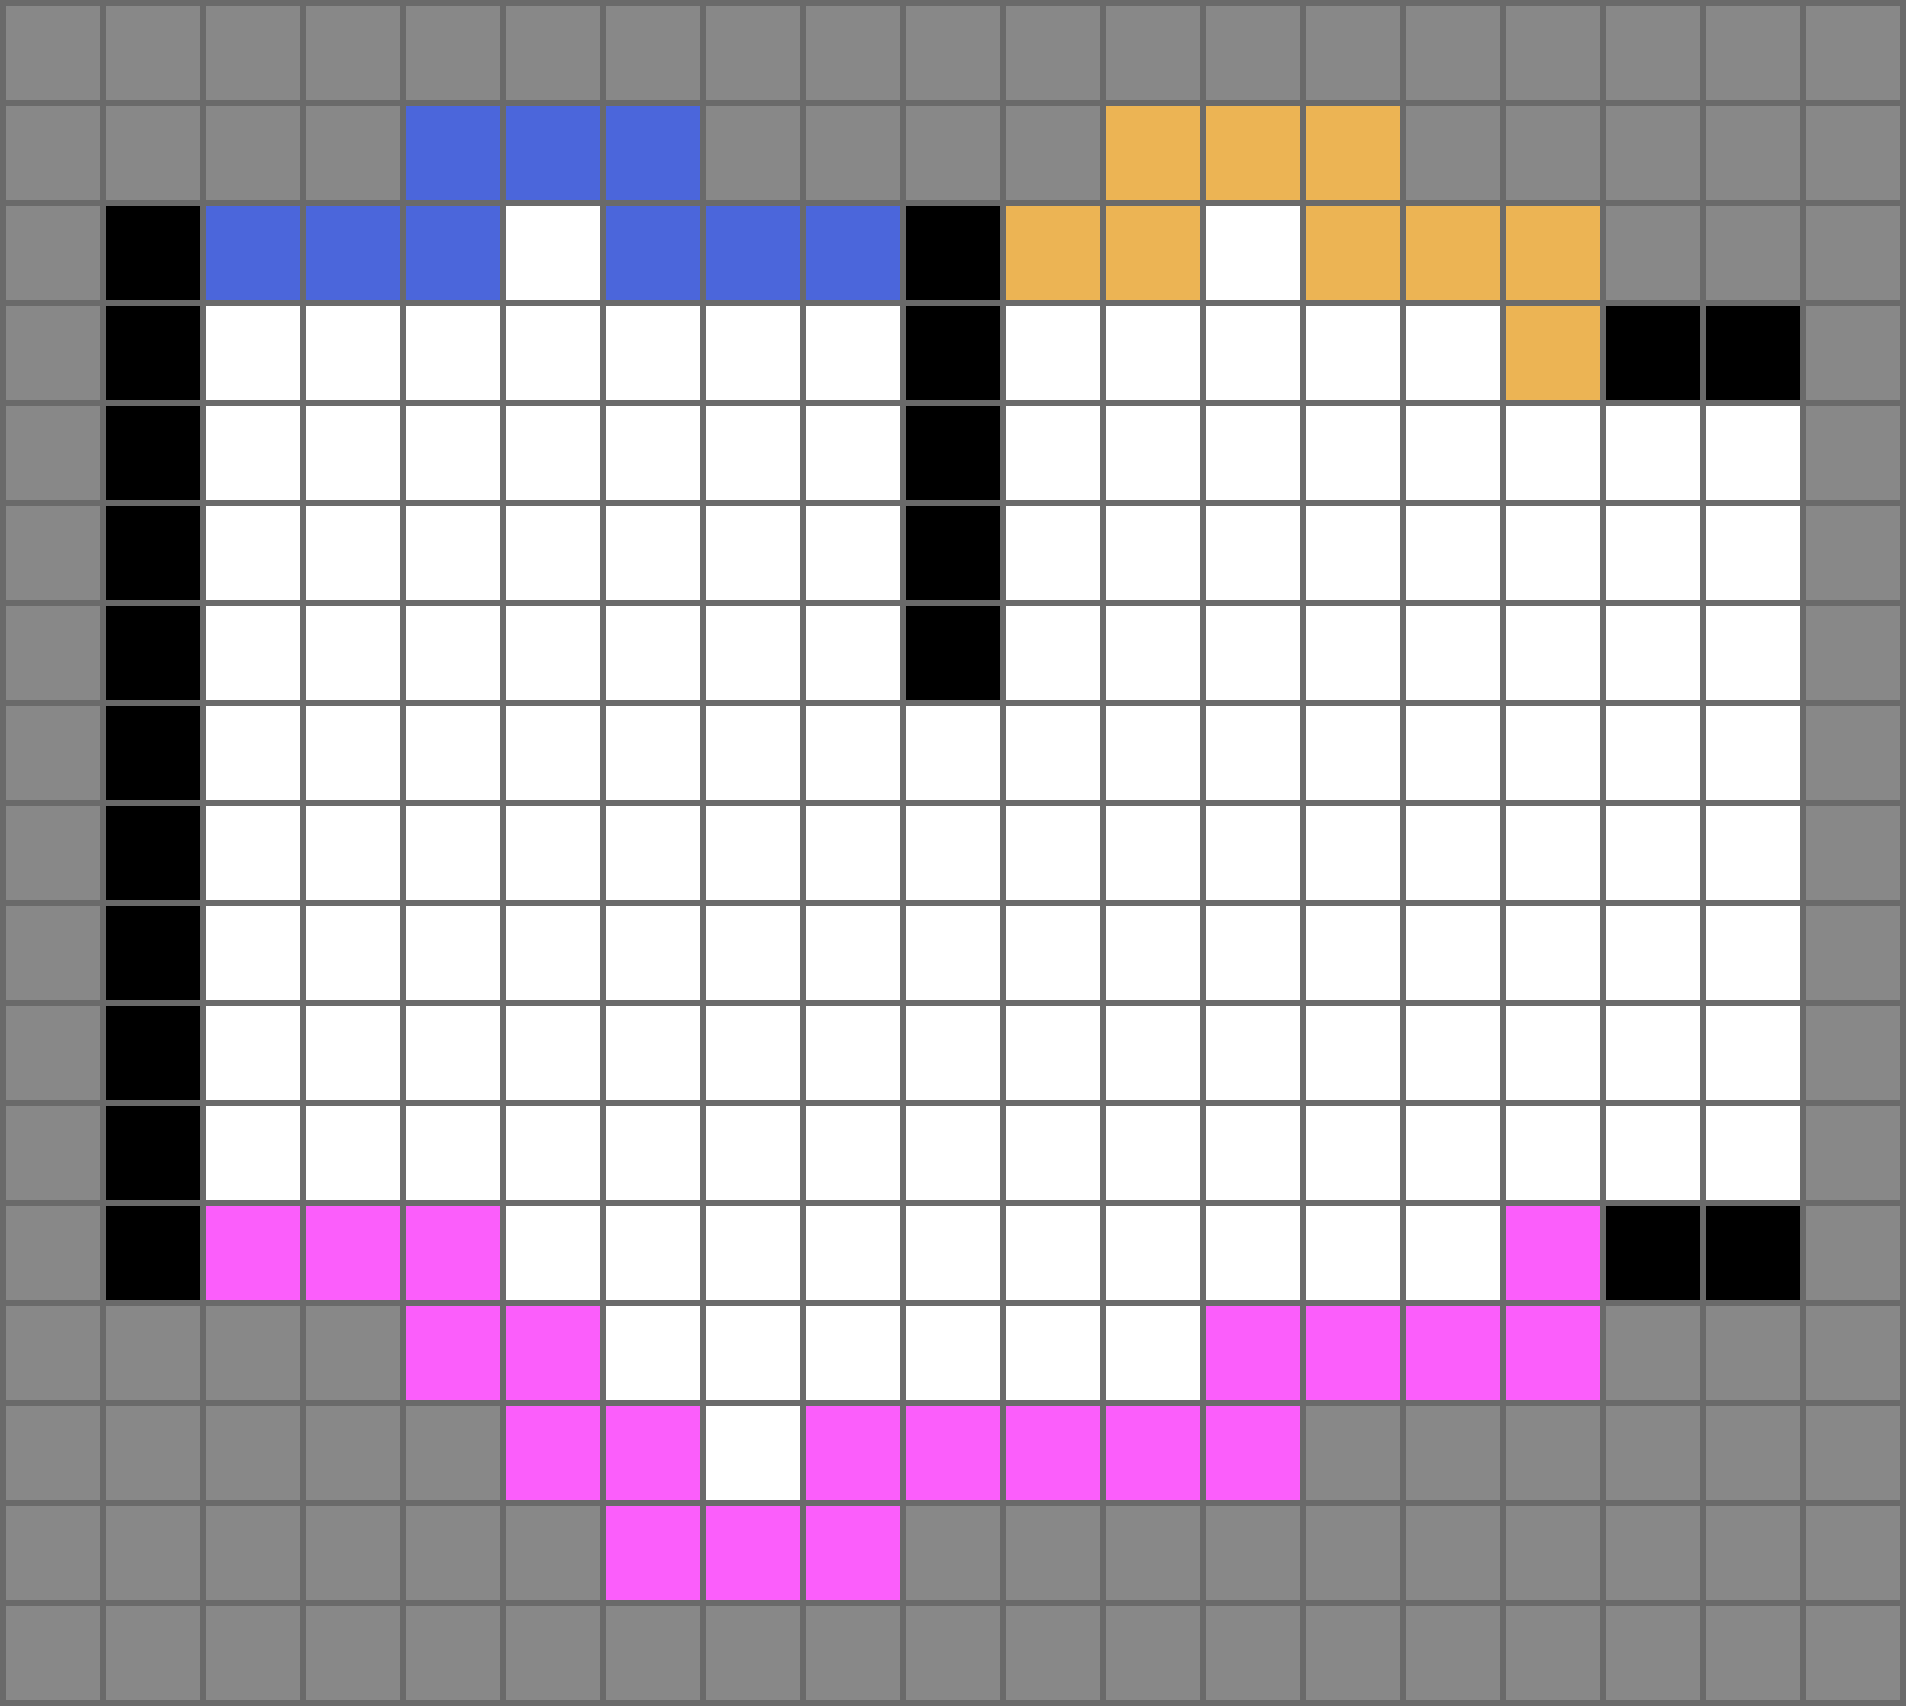
\includegraphics[clip=true, width=0.40\linewidth]{imagenes/fronterasSig/b.png}\label{fig:fronterasCompCon}}
  \qquad
  \subfloat[Fronteras significativas (indicadas con verde) de cada componente conexa.]{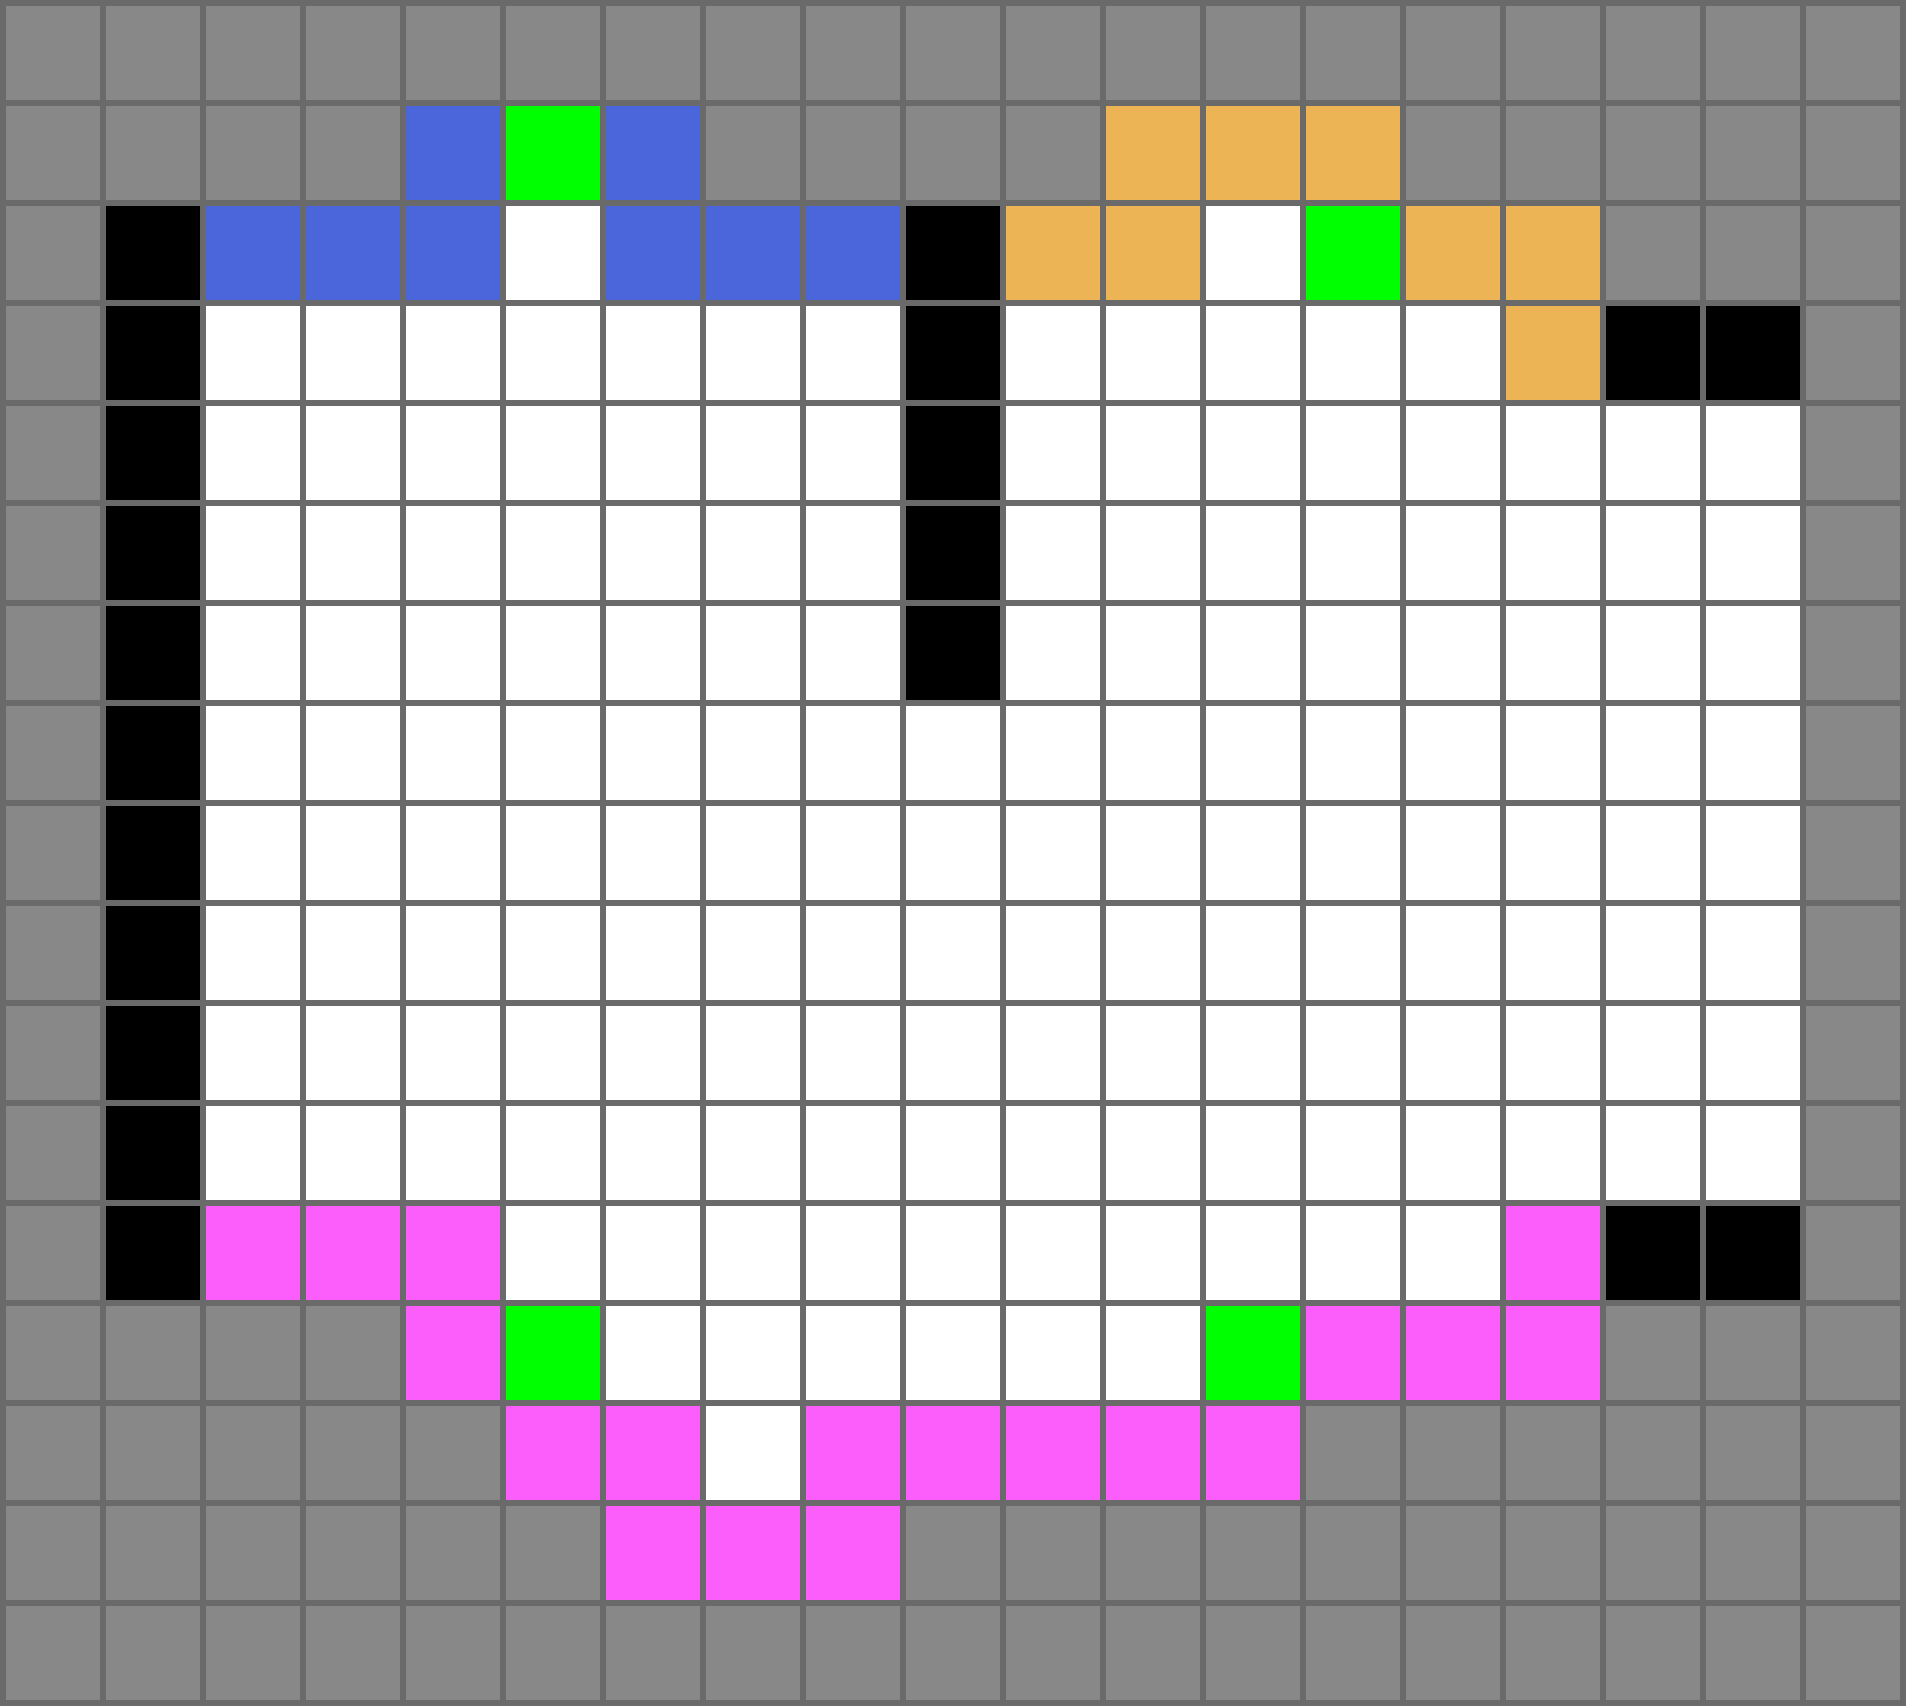
\includegraphics[clip=true, width=0.40\linewidth]{imagenes/fronterasSig/c.png}\label{fig:fronterasSig}}
  \qquad
  \subfloat[Se logra el cubrimiento.]{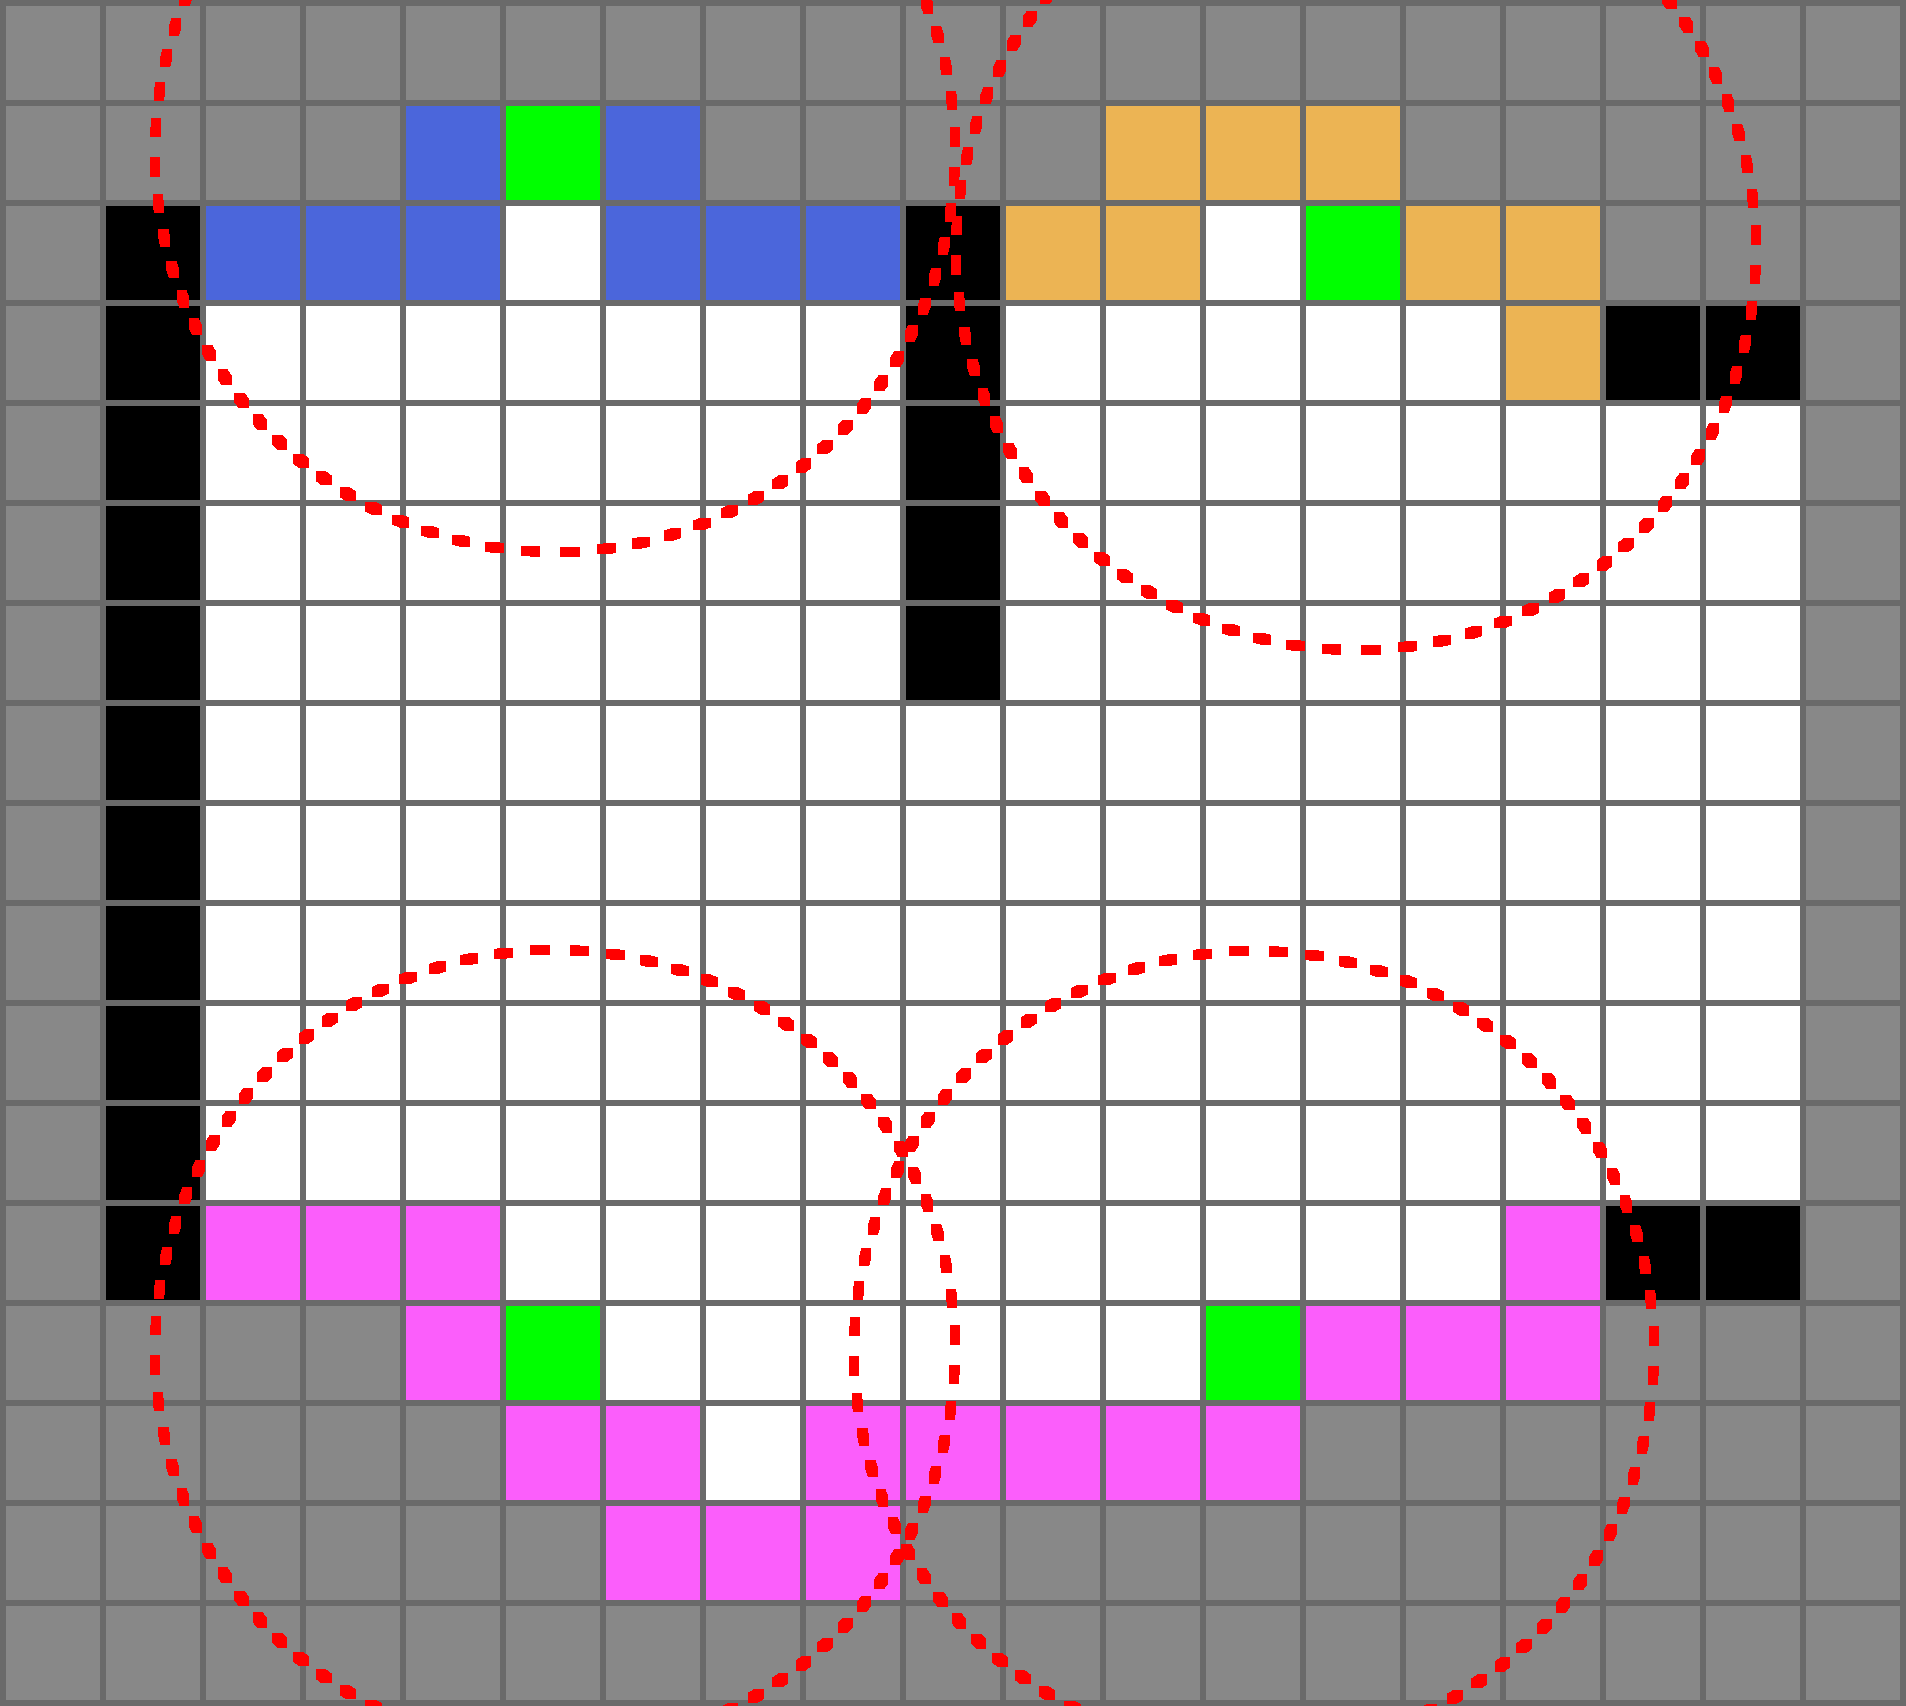
\includegraphics[clip=true, width=0.40\linewidth]{imagenes/fronterasSig/d.png}\label{fig:fronterasSigCub}}

  \caption[Proceso de simplificación de fronteras según K-Means.]{Proceso de
    simplificación de fronteras según K-Means. Las circunferencias rojas
    centradas en las fronteras significativas tienen radio $rango=4$ (largos de celda) indicando su
    cubrimiento. Basado en figuras de \cite{Amorin2019}.}\label{fig:ejemploFrontSig}
  % \caption[Proceso de simplificación de fronteras según K-Means.]{Proceso de simplificación de fronteras según K-Means. Cada figura corresponde a un mismo entorno parcialmente explorado, representado con una grilla, donde las celdas blancas son libres, las negras ocupadas, y para las grises se desconoce su estado. Basada en figuras de \cite{Amorin2019}.}\label{fig:ejemploFrontSig}
\end{figure}

% En la seccion anterior se presento un método que soluciona el siguiente
% problema. Dado un conjunto de  la descomposición en componentes conexas de
% $F$, $\mli{FC}=\{F_1,F_2,...F_N\}$ se obteniene como salida el conjunto
% $\mli{FS} = \bigcup_{i=1}^N \mli{FS_i}$ que cumple con la restriccion de que
% para todo $i \in [1,N]$ $\mli{FS}_i$ cubre a $F_i$.

El problema descrito hasta el momento se puede resumir en el de  dado un
conjunto de fronteras $F$, obtener un conjunto de fronteras significativas
$\mli{FS}$ que cumplen con la restricción de que $\mli{FS}$ cubre a $F$.
Recordando que el propósito de usar $\mli{FS}$ como objetivos de exploración en
lugar de usar $F$ es reducir los objetivos de exploración entonces es natural
pensar que la soluciones optimas reducen al mínimo el $\mli{FS}$ resultante,
mientras mantienen la restricción de cubrimiento.

% Analizando la restriccion de cubrimiento, se puede ver que un indicador de que
% una solucion es subóptima es que varias celdas $\mli{FS}$ se concentren,
% solapandose las circunferencias de radio $rango$ centradas en ellas. Por
% ejemplo 

Dado esto es posible ver que en el ejemplo presentado en
\ref{fig:ejemploFSKMMal} el resultado obtenido por el método presentado en esta
sección no es optimo ya que existen fronteras significativas innecesarias para
el cubrimiento. 

\begin{figure}[H]
  \centering
  \subfloat[Fronteras significativas obtenidas segun el método basado en K-Means.]{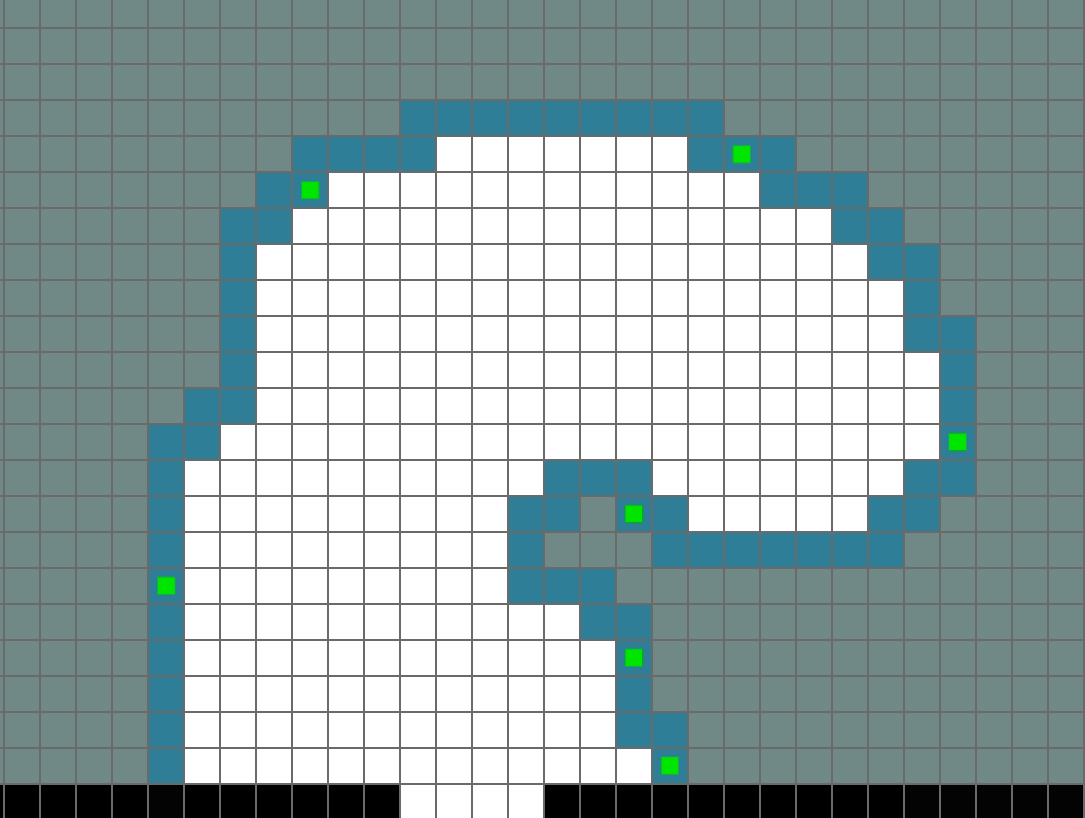
\includegraphics[clip=true, width=0.40\linewidth]{imagenes/fronterasigKMMal/caso1/a_sin_circ.png}}
  \qquad
  \subfloat[Dos de las fronteras significativas de la parte inferior derecha de (a) no son necesarias para lograr el cubrimiento.]{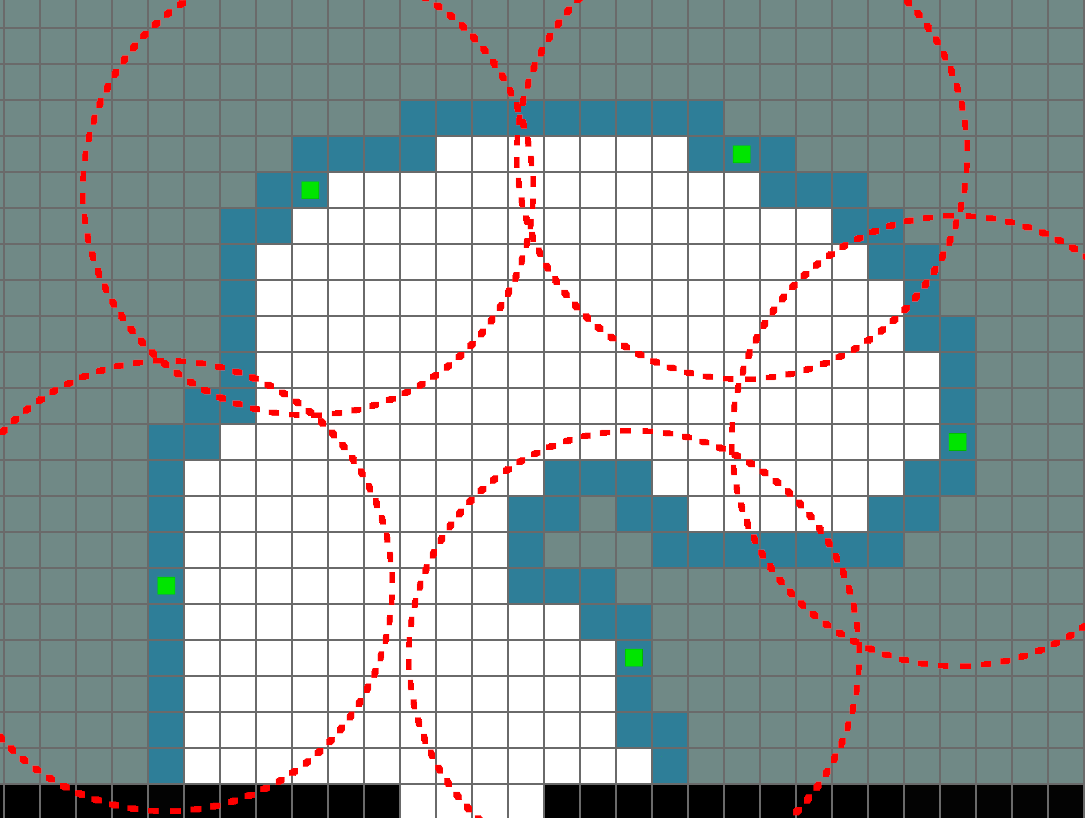
\includegraphics[clip=true, width=0.40\linewidth]{imagenes/fronterasigKMMal/caso1/b.png}}

  \caption[simplificación de fronteras subóptima resultante del método basado en K-Means.]{simplificación de fronteras subóptima resultante del método basado en K-Means. Las fronteras de $F_i$ se indican con azul, las fronteras significativas con verde y las
    circunferencias rojas centradas en estas tienen radio $rango=5.6$ (largos de celda) indicando su
    cubrimiento. Extraída de implementación desarrollada\footnotemark.}\label{fig:ejemploFSKMMal}
\end{figure}
% \footnotetext{Podria indicar el bag y el seg}
%al aplicarse la simplificación 
Resultados subóptimos similares se experimentan de forma consistente sobre
componentes conexas con forma serpenteante asimétricas y lo suficientemente
extensas como para requerir más de 4 fronteras significativas para su
cubrimiento, 
%con un largo mayor a $rango*8$ 
% \todo[inline]{se entiende la idea del largo aplicada a esto? Creo que puede
% quedar claro mirando la foto pero tengo mis dudas. La idea en realidad sería
% decir que la solucion no es lo suficientemente simple, por ejemplo si con 1
% sola frontera sig ya se cubre todo entonces no va haber problema sin importar
% que tan serpenteante o asimetrica sea. Se me ocurre que puedo tratar la simpleza hablando por el largo puede
% quedar más claro o más oscuro, es decir por que 8? fue para poner un valor
% similar al de la foto que necesita 5 fronteras para cubrir }
empeorando (mayor cantidad de fronteras significativas
innecesarias para el cubrimiento) a medida que las componentes conexas de
fronteras son más extensas y las curvas son más intrincadas.

% (comentarlos, distribuciones desparejas, acumulacion, no
% equidistantes) 

% Una explicacion posible a este comportamiento es que la distibucion de centroides en K-Means 

% Algo que se repite en estas situaciones es que suele haber zonas, en donde las
% fornteras significativas se acumulan, y zonas en las que estan muy dispersas
% (casi a $rango$ de distancia una de la otra, el maximo). Esto lleva a pensar que K-Means se tiende a ubicar concentrar los centroides en una zona,

Esto se presume que se debe principalmente a dos factores relacionados a
K-Means. (i) K-Means no considera la restricción de cubrimiento para generar sus
resultados. La restricción se fuerza ejecutando K-Means con el mínimo $k$
(obtenido con prueba y error) según el cual las fronteras significativas
resultantes logran el cubrimiento. (ii) Los centroides resultantes de K-Means
no son fronteras. Estos se deben traducir a fronteras posteriormente.

% \todo{Hay una arbitrariedad asociada a k-means tambien lo cual puede ser criticado tambien, aunque deberia estudiar mejor el tema, quizas no criticarlo aca pero destacar que el otro método es menos opaco en como elige las front sig}
% Esto es la clase de pe la idea de obtener fornteras significativas es reducir el numero
% de objetivos de exploración,

% El método basado en K-Means aunque funciona bien al aplicase en componentes conexas pequeñas, 

% El método descrito en la seccion resulta en un conjunto de fronteras
% significativas que cubren a las fronteras, el problema que se detecto
% experimentalmente es que en ciertos casos el resultado  la discribucion de las
% fronteras significativas es mala, se concentran mucho en ciertas porciones y se alejan 

\subsection{Simplificación de fronteras basada en cubrimiento}\label{subsec:MiSimp}
Con esto en mente se desarrolla un método novedoso que considera los dos puntos
destacados anteriormente. (i) Tomando en cuenta el cubrimiento y su
optimización como parte fundamental del algoritmo. (ii) Dando directamente
fronteras como resultado.

El algoritmo al igual que el descrito en la sección anterior comienza
descomponiendo a las fronteras $F$ en sus componentes conexas
$\mli{FC}=\{F_1,F_2,...F_N\}$ para luego obtener las fronteras significativas
$\mli{FS}_i$ para cada componente $F_i$, siendo el conjunto total de fronteras
significativas $FS = \bigcup^N_{i=0} \mli{FS}_i$

El proceso completo que permite obtener las frontera significativas
$\mli{FS}_i$ para un componente $F_i$ se muestra en el algoritmo
\ref{alg:IdObjGeo}.

\begin{algorithm}[H]
\SetAlgoLined
  \SetKwInOut{Input}{Entrada}
  \Input{$F_i$}

  $\mli{UF} := F_i$ \\
  $\mli{FS}_i := \emptyset$\\

  $\mli{PF} :=$ Cola vacía \\
  \ForEach { $f\in F_i$ } {
    \ForEach{ $\mli{fa} \in ady(f)$ } {
      \If { $e(\mli{fa}) = ocupado$ } {
        $\mli{PF}.encolar(f)$
      }
    }
  }
  \If{$\mli{PF}.vacia()$}{
    $\mli{PF}.encolar($elemento arbitrario de $F_i)$
  }
  \While{$\mli{UF} \neq \emptyset$ } {
    $\mli{pf} := \mli{PF}.desencolar()$\\
    \If{ $\mli{pf} \in \mli{UF}$}{
      $dCen := max \{ d_{\mli{pf}}(\mli{f}) : f\in\mli{UF} \}/2$\\
      $radio := min \{dCentrada, rango\}$\\
      $\mli{FSC} :=\mli{UF} \cap \mathscr{C}(\mli{pf},radio)$\\
      $\mli{fs} := $elemento arbitrario de $\mli{FSC}$\\
      $\mli{FS_i} := \mli{FS_i} \cup \{\mli{fs}\}$\\

      $\mli{RC} := \{ f\in F_i : d_{\mli{fs}}(f) \leq rango\}$\\

      $\mli{UF} := \mli{UF} - \mli{RC}$\\

      \ForEach { $\mli{pf} \in \{ f \in \mli{UF} : \exists c \in \mli{RC}, f \in ady(c)\}$}{
        $\mli{PF}.encolar(\mli{pf})$
      }
    }
  }
  \Return $\mli{FS}_i$ 

  \caption{simplificación de fronteras basada en cubrimiento}
  \label{alg:IdObjGeo}
\end{algorithm}

Para obtener las fronteras significativas de $F_i$ el algoritmo parte mantiene
las fronteras significativas determinadas $\mli{FS}_i$, el conjunto
todas las fronteras que resta cubrir $\mli{UF}$ (siglas del ingles
\emph{uncovered frontiers}), y  una cola FIFO $\mli{PF}$ en donde se almacenan 
los próximas fronteras a cubrir.

$\mli{FS}_i$ se inicializa vacía y $\mli{UF}$ como $F$ (líneas 1 y 2). Por otro
lado $\mli{PF}$ se inicializa encolando en cualquier orden a las celdas
fronteras adyacentes a celdas cuyo estado es ocupado, de no existir ninguna se
encola una única frontera arbitraria de $F_i$ (líneas 3-13). 

Luego el algoritmo se basa en elegir una frontera de $\mli{UF}$ como frontera
significativa $\mli{fs}$ (líneas 15-20). Posteriormente se actualizan las
estructuras mantenidas en función de la nueva $\mli{fs}$ (líneas 21-27), notar
que esto implica reducir el numero de celdas en $\mli{UF}$ ya que como mínimo
$\mli{fs}$ se cubre a si misma. Este proceso de elección y actualización se
repite hasta que $\mli{UF}$ queda vacía (línea 14). Luego de lo cual se
devuelven las fronteras significativas $\mli{FS_i}$ resultantes (línea 29).
 
Ahora se profundizara sobre los procesos de elección (líneas 15-20) y
actualización (líneas 21-27).

El proceso de elección de $\mli{fs}$ utilizado tiene como objetivo el asegurar
que se cubra una frontera previamente no cubierta $\mli{pf}$ (obtenida de
desencolar a $\mli{PF}$), esto se traduce en la restricción
$d_{\mli{pf}}(\mli{fs}) \leq rango$. Adicionalmente se tiene una heurística que
establece que dado $dCen = max\{ d_{\mli{PF}}(\mli{f}) : f\in\mli{UF} \}/2$ las
fronteras que estén a $min \{dCen, rango\}$ de distancia de $\mli{pf}$ serán las
mejores candidatas a ser fronteras significativas. La heurística busca elegir a
las fronteras significativas que queden en el centro del conjunto de celdas
nuevas que van a cubrir de $\mli{UF}$. Con esto en cuenta se determina un
conjunto de de fronteras significativas candidatas $\mli{FSC}$ como el conjunto
de celdas que pertenecen a $\mli{UF}$ y a la circunferencia discretizada
de $radio = min \{dCen, rango\}$ centrada en $\mli{PF}$ denotada como
$\mathscr{C}(\mli{pf},rango)$ (\ref{eq:cir}).
% \todo[inline]{este concepto capaz no queda claro. Es muy específico y
% explicarlo me paree que corta un poco la narrativa. Dado el conjunto
% $Cir=\{f\in F_i : d_{\mli{pf}}(f) \leq radio\}$ son los puntos de $Cir$ que
% tienen un adyacente fuera de $Cir$ }
\begin{equation} \label{eq:cir}
\begin{aligned}
&\mathscr{D}(\mli{pf},rango) = \{c\in\mli{CG} : d_{\mli{pf}}(c) \leq radio\}\\ 
&\mathscr{C}(\mli{pf},rango) = \{c\in\mathscr{D}(\mli{pf},rango) : \exists cA \in ady_8(c), cA \notin \mathscr{D}(\mli{pf},rango) \}
\end{aligned}
\end{equation}

Finalmente para elegir una nueva frontera
significativa $\mli{fs}$ se debe elegir una frontera de $\mli{FSC}$, en esta
propuesta la elección se hace de forma arbitraria.

El proceso de actualización consiste en agregar $\mli{fs}$ a $\mli{FS}_i$, obtener el
conjunto de fronteras cubiertas por $\mli{fs}$ las que se denominan como
$\mli{RC}$ (siglas de recién cubiertas), las cuales se deben remover de
$\mli{UF}$ y se utilizan para determinar que celdas encolar a $\mli{PF}$.
El encolar nuevas fronteras en $\mli{PF}$ es necesario para que el criterio de
elección propuesto funcione de forma correcta, siendo las fronteras agregadas
para ser cubiertas en próximas iteraciones las fronteras en $\mli{UF}$ que son
adyacentes a las fronteras recién cubiertas.

Un ejemplo de ejecución para el caso presentado en la figura
\ref{fig:ejemploFSKMMal} se muestra en la figura \ref{fig:ejemploFSCub}. En el
apéndice \ref{EXE:sfbc} se muestra la misma ejecución con un mayor nivel de
detalle.

\begin{figure}[H]
  \centerfloat
  \subfloat[Incializacion de $\mli{PF}$, $\mli{UF}$ y $\mli{FS_i}$.]{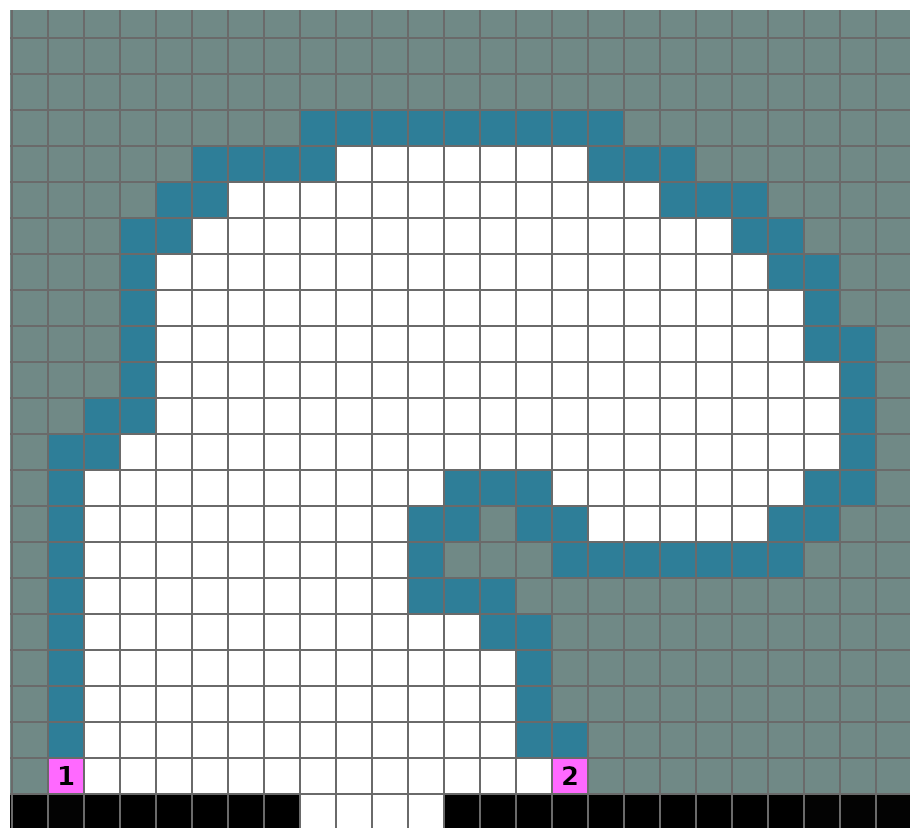
\includegraphics[clip=true, width=0.40\textwidth]{imagenes/ejemploSimpCub/a2.png}}
  \subfloat[Se elige un nuevo $\mli{fs}$ y se actualizan $\mli{UF}$, $\mli{FS_i}$ y $\mli{PF}$.]{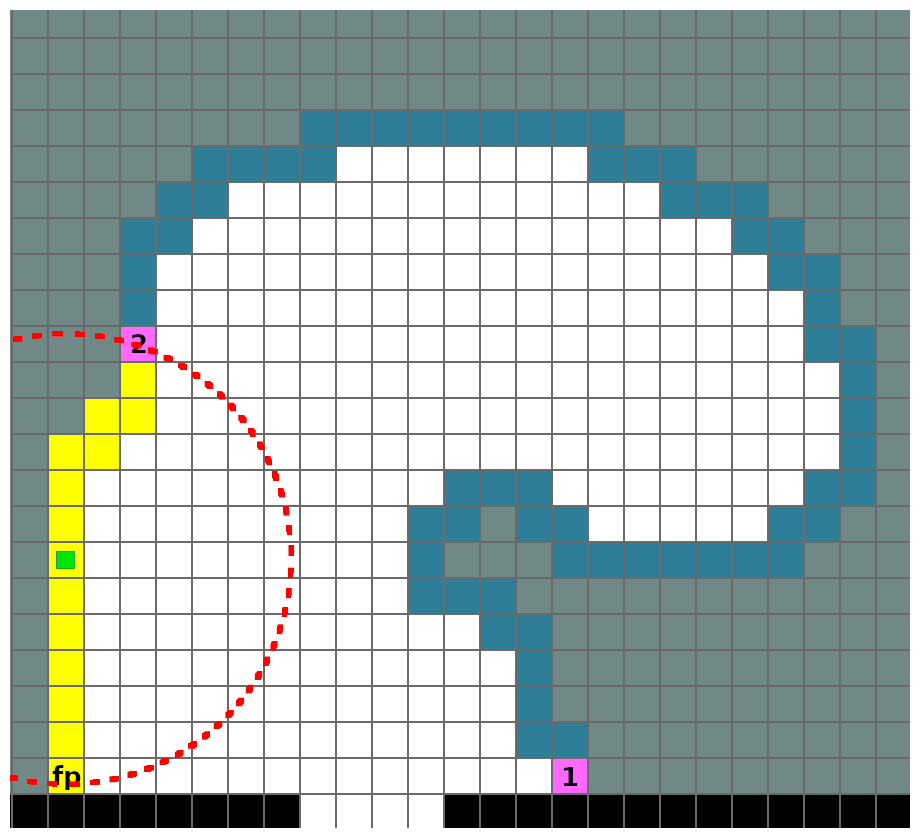
\includegraphics[clip=true, width=0.40\textwidth]{imagenes/ejemploSimpCub/b5.png}}
  \subfloat[Se elige un nuevo $\mli{fs}$ y se actualizan $\mli{UF}$, $\mli{FS_i}$ y $\mli{PF}$.]{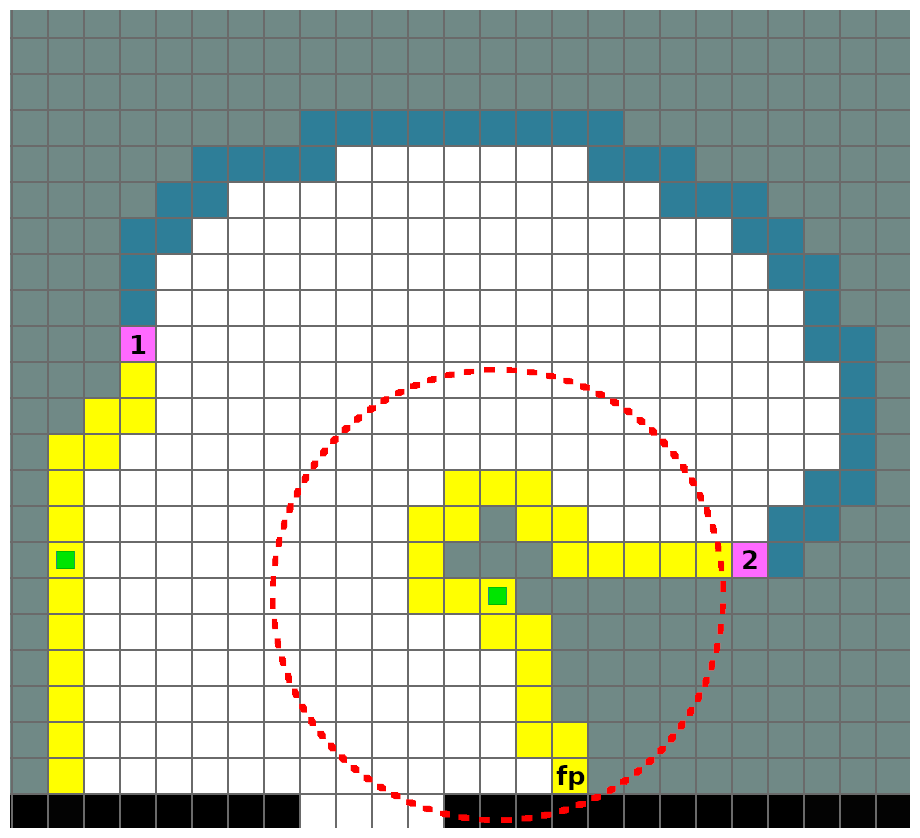
\includegraphics[clip=true, width=0.40\textwidth]{imagenes/ejemploSimpCub/c5.png}}

  \subfloat[Se elige un nuevo $\mli{fs}$ y se actualizan $\mli{UF}$, $\mli{FS_i}$ y $\mli{PF}$.]{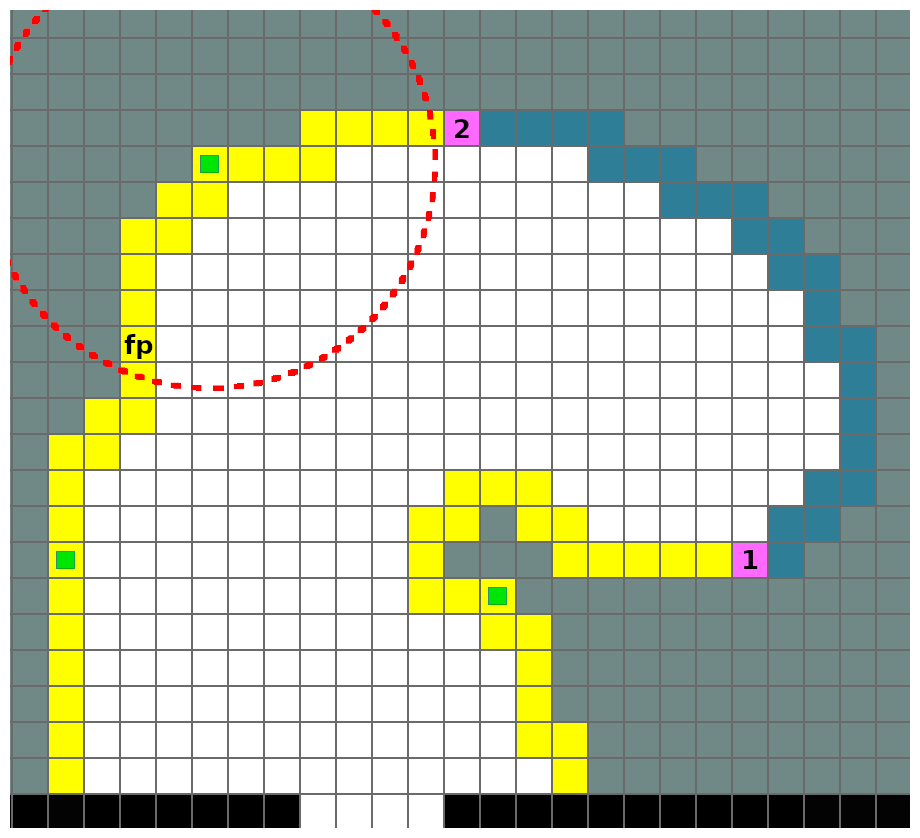
\includegraphics[clip=true, width=0.40\textwidth]{imagenes/ejemploSimpCub/d5.png}}
  \subfloat[Se elige un nuevo $\mli{fs}$ y se actualizan $\mli{UF}$, $\mli{FS_i}$ y $\mli{PF}$.]{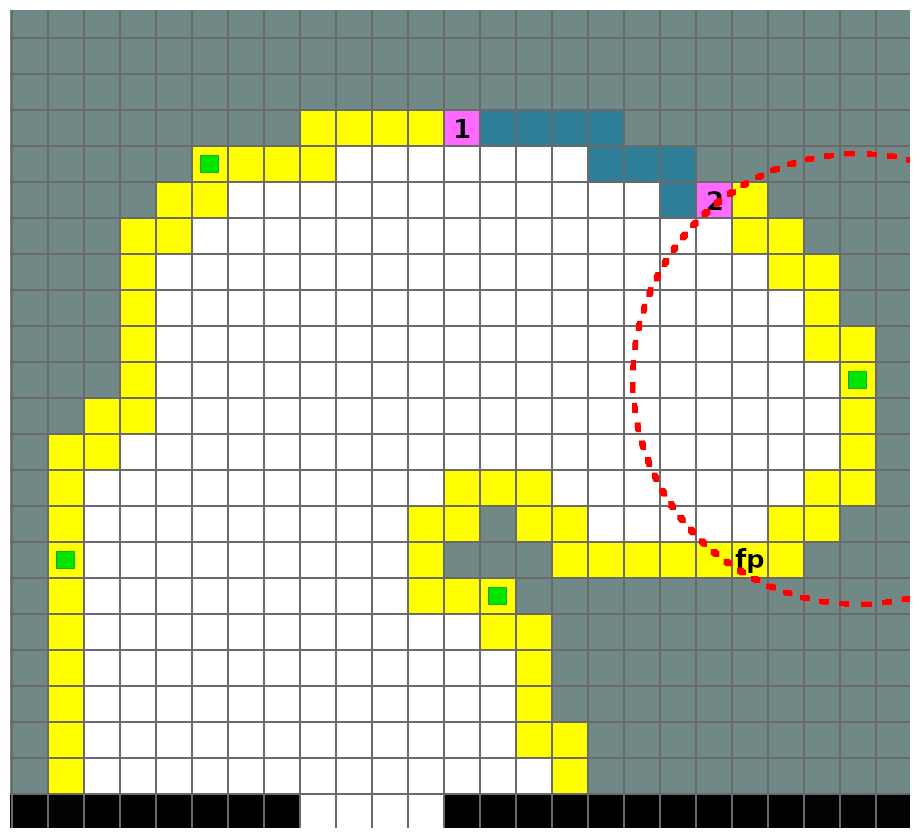
\includegraphics[clip=true, width=0.40\textwidth]{imagenes/ejemploSimpCub/e5.png}}
  \subfloat[Se elige un nuevo $\mli{fs}$ y se actualizan $\mli{UF}$, $\mli{FS_i}$ y $\mli{PF}$.]{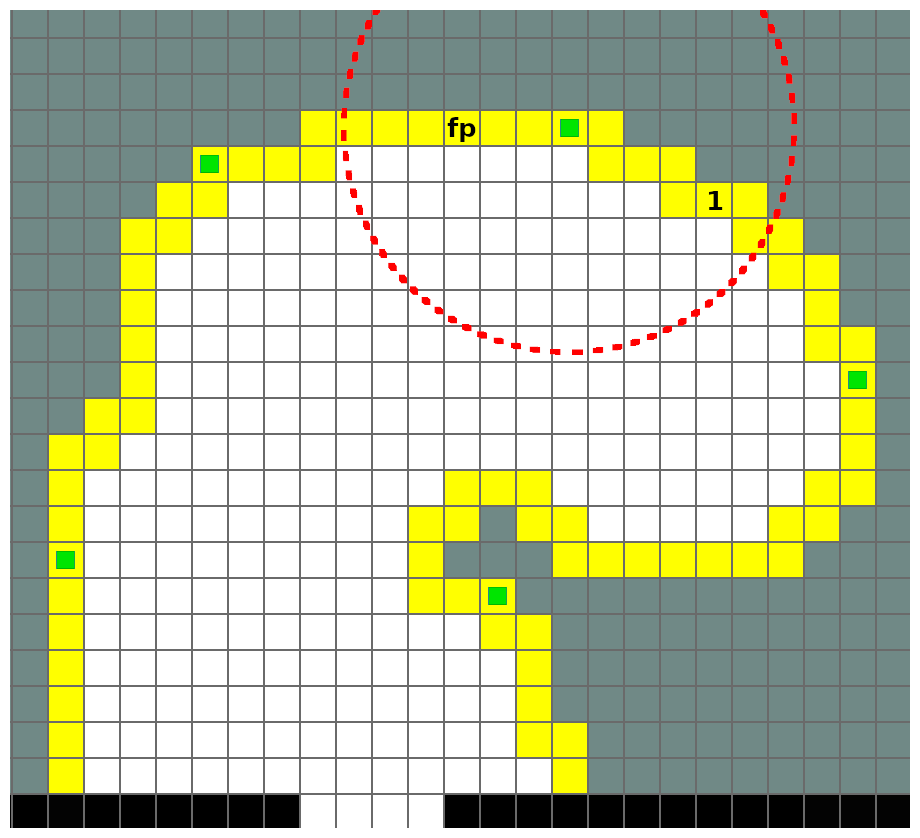
\includegraphics[clip=true, width=0.40\textwidth]{imagenes/ejemploSimpCub/f4.png}}

  \subfloat[$\mli{UF}=\emptyset$ por lo que el algorimo finaliza.]{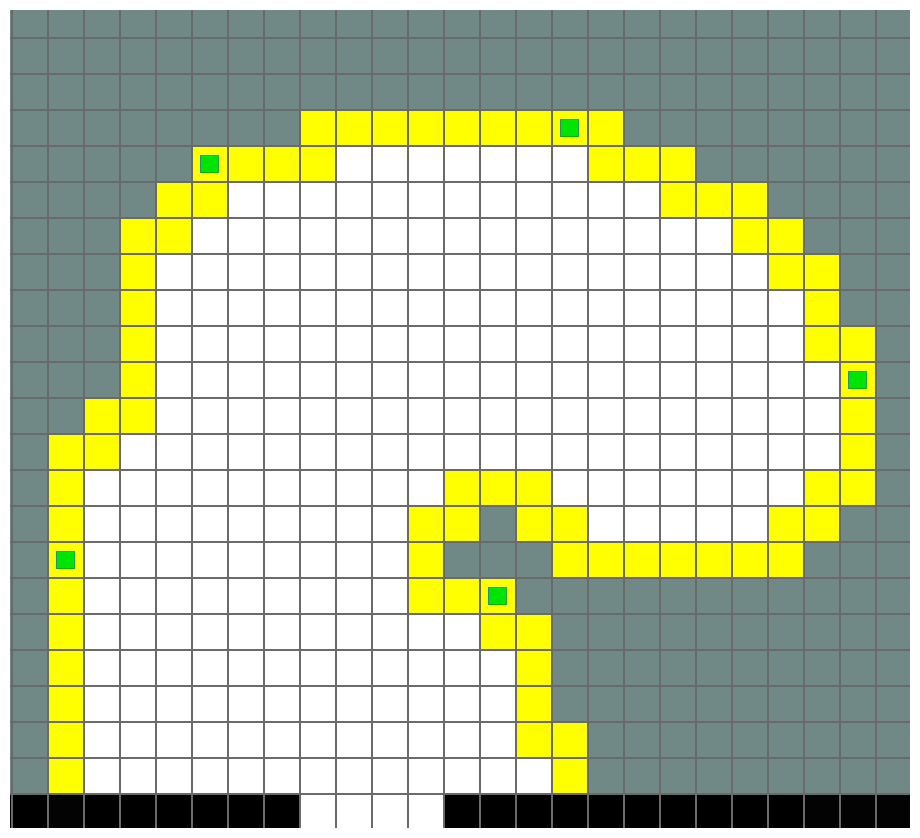
\includegraphics[clip=true, width=0.40\textwidth]{imagenes/ejemploSimpCub/zfinal1.png}}
  \subfloat[Resultado final.]{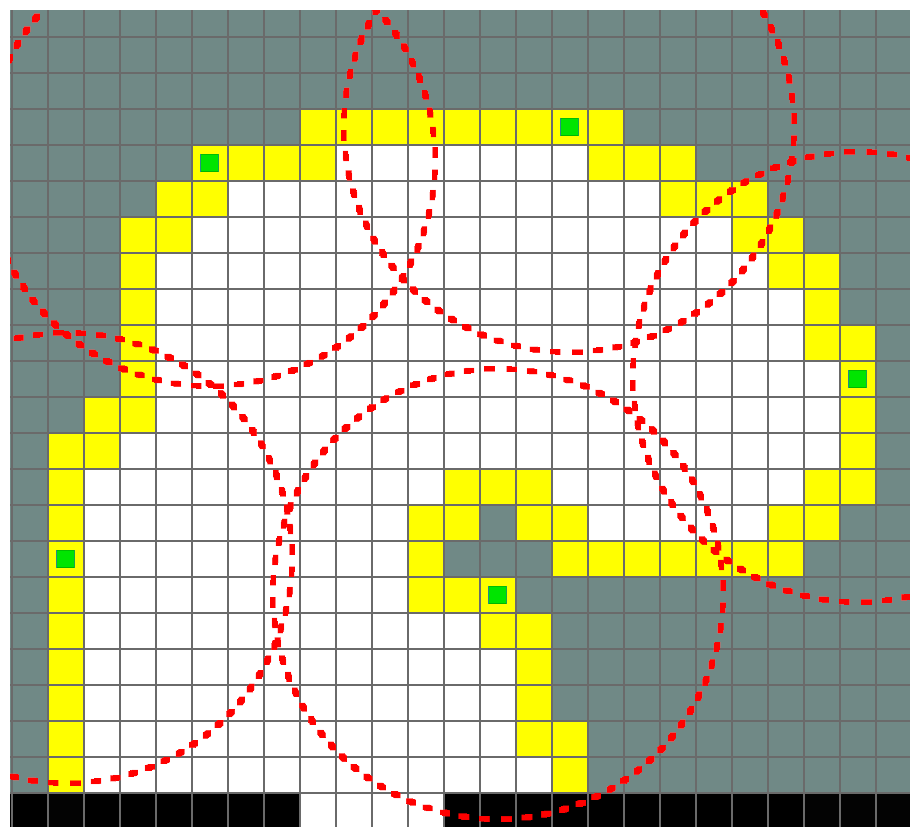
\includegraphics[clip=true, width=0.40\textwidth]{imagenes/ejemploSimpCub/zfinal2.png}}

  \caption[Proceso de simplificación de fronteras según cubrimiento.]{Proceso
    de simplificación de fronteras según cubrimiento.  Las fronteras de
    $F_i$ se indican con azul si pertenecen a $\mli{UF}$ y con amarillo de lo
    contrario. Con magenta se indican las celdas en $\mli{PF}$ siendo la
  numeración su orden en la cola y $\mli{pf}$ la ultima desencolada. Las fronteras significativas se indican con
verde, siendo las circunferencias rojas de radio $rango=5.6$ (largos de celda) centradas en estas indicadores de su cubrimiento.}\label{fig:ejemploFSCub}

\end{figure}


\section{Asignación de objetivos}\label{sec:asigTar}

Cuando un robot se encuentra ocioso este le solicita a la central que le asigne
un nuevo objetivo, esto desencadena el proceso de asignación de
objetivos que se describe a lo largo de esta sección.

La asignación de objetivos se basa en la estrategia de coordinación presentada
en \ref{subsec:wurmCoord}, que sostiene que es conveniente que los robots se
asignen a los objetivos de forma que estos se distribuyan uniformemente sobre
las habitaciones y corredores (segmentos) de un entorno estructurado, que se
corresponden las regiones de un mapa topológico (sección \ref{subsec:mapas}).

La asignación de objetivos consiste una subasta donde los objetivos de
exploración son subastados entre los robots. La subasta se puede separar en
tres partes, \emph{obtención de información}, \emph{valuación} y
\emph{resolución}. La \emph{obtención de información}, es la etapa en la cual
todos los datos necesarios para llevar adelante la subasta (por ejemplo los objetivos de
exploración) son determinados. La \emph{valuación} abarca la distribución de
la información obtenida desde la central hacia los robots, el juicio de valor
de cada robot a cada objetivo recibido y el posterior envió de estas
valoraciones desde los robots hacia la central. La \emph{resolución} contempla
la recepción de las valoraciones por la central, un postprocesamiento sobre
estos, la asignación de objetivos a robots según la valoraciones y los
segmentos a los cuales pertenece cada objetivo, finalizando con la notificación
del objetivo que le fue asignado a cada robot.

Con respecto a la separación del problema de asignación de objetivos mencionada
en la sección \ref{sec:exploracion}, la parte de identificación de objetivos
esta incluida en la \emph{obtención de información}, y la parte de
distribución de objetivos se corresponde con el el resto de lo que se describe
en esta sección.

\subsection{Obtención de información}\label{subsec:obtInfo}
%, esto desencadena una nueva subasta de no encontrarse una en curso.
% Notar que si existe una subasta en curso el robot va recibir un objetivo cuando
% esta termine, por lo que puede no ser necesario iniciar otra.
Como se menciono anteriormente cuando un robot ocioso solicita un objetivo a la
central se da comienzo a una nueva subasta.
La etapa de \emph{obtención información} es la primera etapa de la subasta. La
información que se obtiene en esta etapa son los objetivos de exploración, un
GVD y los segmentos del entorno explorado.
% que con el motivo
% de identificar en que segmento se encuentra cada objetivo de exploración, para
% posteriormente poder distribuir a los robots sobre estos. 

La identificación de objetivos se lleva a cabo con el método descrito en la
sección \ref{subsec:MiSimp}.

La identificación de los segmentos se logra aplicando una técnica que se basa
en la propuesta de \cite{Thrun1998} explicada en la sección
\ref{subsec:mapaTopGVD}. Detalles de como esta técnica fue implementada se
presentan en la sección \ref{subsec:mapaTopGVDGrid}. 

El GVD requerido para identificar los segmentos se construye de forma
incremental con una variante del \emph{brushfire dinámico} que se comenta en la
sección \ref{sec:MiConstGVD}.
% de no de los cambios principales con
% respecto al trabajo original de \cite{wurm2008coordinated} es la forma en la
% cual se contruye el GVD. En el trabajo original se hace uso de un método de
% construccion no incremental, en este proyecto con el motivo de alcanzar una
% implementación eficiente para su uso en tiempo real (seccion
% \ref{subsec:constGVDInc})

\subsection{Valuación} \label{subsec:MiValSub}

Luego de obtenida la información comienza la etapa de \emph{valuación}
con la central distribuyendo los objetivos y el GVD hacia los robots. Cuando un
robot recibe la información este asigna dos valores a cada objetivo, el largo
del camino hacia a el y un costo asociado a la complejidad del camino.

Calcular el largo de un camino implica determinar el camino en sí. En este
proyecto los caminos se componen de una secuencia de puntos en el espacio que
comienza en la posición del robot y termina en el objetivo. Los caminos se
calculan de forma distinta dependiendo de la clase de objetivo al que llevan,
existiendo dos clases, trivial y no trivial.

Los objetivos triviales se definen como los objetivos para los cuales el
segmento de recta que existe entre el robot y el objetivo no contiene
obstáculos, de lo contrario el objetivo es no trivial. Para determinar esto, se
discretiza el segmento de recta en celdas \cite{foleyphillips} y se comprueba
en el mapa global (grilla de ocupación) almacenado en el robot, alguna de las
celdas tiene un estado ocupado. 

El camino hacia objetivos triviales se determina como los puntos ubicados en
los extremos del segmento de recta que existe entre el robot y el objetivo, que
se encuentra libre de obstáculos. Un ejemplo de un camino trivial se muestra
en la figura \ref{fig:caminoT}.

En el caso de los objetivos no triviales se hace uso del GVD recibido como
parte de la información de la subasta, aprovechando que este constituye un
\emph{roadmap} (sección \ref{subsec:mapacarr}). El proceso para construir el
camino puede dividir en tres partes cada una asociada a una de las propiedades
que caracterizan a un \emph{roadmap}: accesibilidad, conectividad y capacidad
de salida. La parte asociada accesibilidad consiste en encontrar un camino
desde el robot al GVD, lo cual se hace a través de un \emph{breadth-first
search} (BFS), comenzando en la celda asociada a la posición del robot y
deteniéndose apenas se visita una celda $c_1$ perteneciente al GVD. La que se
relaciona con la capacidad de salida es análoga a la accesibilidad pero el
desde el objetivo a alguna celda $c_2$ perteneciente al GVD. Por ultimo la parte
vinculada con la conectividad se basa en establecer un camino sobre las celdas
pertenecientes al GVD desde $c_1$ a $c_2$, lo cual se hace aplicando algoritmo
$A^*$. Conectando los centros de celdas de estos tres caminos se obtiene el
camino completo. En la figura \ref{fig:caminoNT} se presenta un ejemplo de un
camino no trivial.

\begin{figure}[H]
  \centerfloat

  \subfloat[Trivial.]{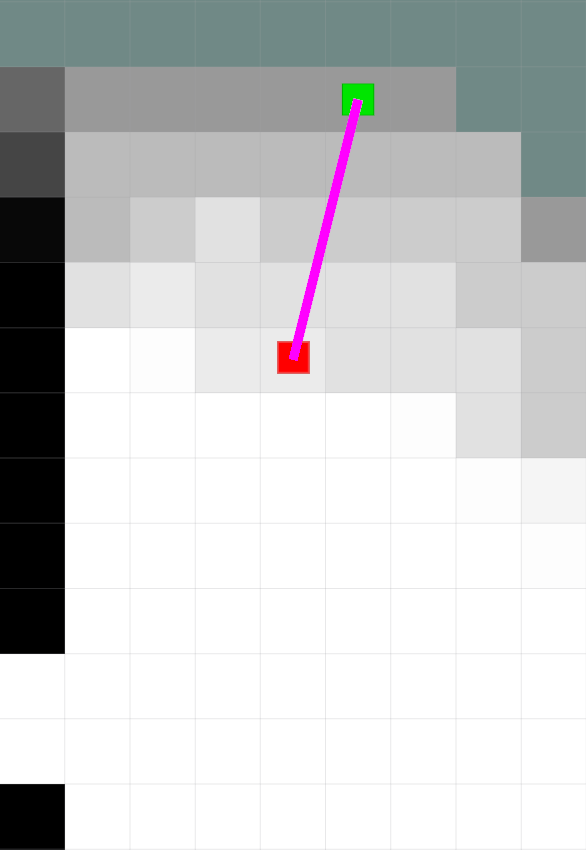
\includegraphics[clip=true, width=0.25\textwidth]{imagenes/camino/caminoTsinGVDRecortado.png}\label{fig:caminoT}}
  \qquad
  \subfloat[No trivial.]{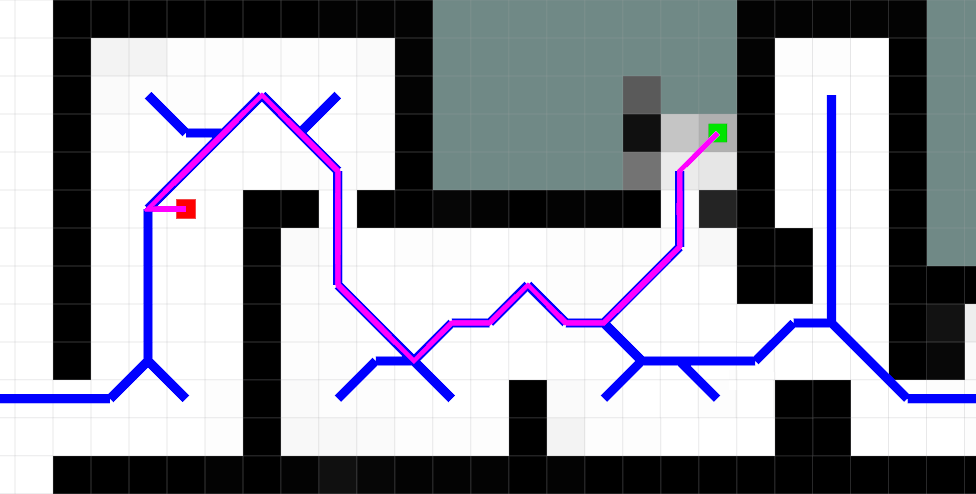
\includegraphics[clip=true, width=0.70\textwidth]{imagenes/camino/camino.png}\label{fig:caminoNT}}

  \caption[Camino.]{Caminos calculados desde la posición del robot indicada en
  rojo, hasta el objetivo indicado en verde. Los puntos del camino se conectan
entre si con líneas magenta.}\label{fig:camino}

\end{figure}


El costo asociado a la complejidad en el caso de objetivos triviales se
corresponde a una estimación del tiempo que demora el robot en rotar de forma
que su parte delantera apunte hacia el objetivo. Y en el caso de objetivos no
triviales se utiliza la maxima penalización usada para objetivos no triviales.
El propósito de esto es diferenciar los objetivos triviales sin beneficiar a
los objetivos no triviales. Este costo se aplica para incentivar a que el robot
continue siendo asignado a los objetivos triviales que tiene por adelante al
explorar.

Obtenidos ambos valores para cada objetivo estos se envían hacia la central
junto a la ubicación actual del robot, siendo toda esta información en su
conjunto considerada una valuación. %\todo{o mensaje de valuación, como quede mejor}

% De esta
% forma los objetivos triviales se valuan distinto segun que tanto tiene que
% rotar el robot para llegar a ellos y los objetivos no triviales tendran un
% costo no mayor al del peor objetivo no trivial.

% como el conjunto de celdas que abarca, el proceso para construir el camino es
% se puede dividir en encontrar tres subcaminos cada uno relacionado a una de las
% tres propiedades de un roadmap: accesibilidad, conectividad y capacidad de
% salida. La accesibilidad consiste en encontrar un camino desde el robot al GVD,

% La valuacion abarca la distribuicion de los objetivos de exploración desde la
% central hacia los robots, la asignación de valores que cada robot debe hacer a
% cada objetivo y el posterior envio de estas valoraciones desde los robots hacia
% la central. 

\subsection{Resolución} \label{subsec:MiResSub}
La resolución comienza con la central recibiendo las valuaciones realizadas por
los robots. Al recibirse la primera valuación existe una ventana de tiempo en
la que la central continuara recibiendo nuevas valuaciones. Terminada esta
ventana se ejecuta un algoritmo que resulta en la asignación de objetivos a los
robots. Finalmente las asignaciones realizadas son comunicadas a los robots.
% La resolución es el proceso de asignar los objetivos La resolución contempla
% la recepción de las valoraciones por la central, la asignación de objetivos a

% robots según y la notificación del objetivo asignado a los robots. 
% de exploración a los
% robots. 
\subsubsection{Recepción de valuaciones}
Como se menciono anteriormente luego de recibida la primera valuación existe
una ventana de tiempo en la que la central continuara recibiendo nuevas
valuaciones luego de la cual se da por concluida la recepción de valuaciones. 

El propósito de utilizar una ventana es que en escenarios reales los robots
pueden dejar de comunicarse por alguna razón (desconexiones de red, accidentes
que dejen a los robots sin funcionar, entre otros), por lo tanto esperar por
las valuaciones de todos los robots puede ser una espera infinita.

Dado que el problema que los robots deben resolver para generar las valoraciones es
similar, se asume que el tiempo se demora en generar las valoraciones también
es similar, adicionalmente dicho tiempo es proporcional al area del
mapa que se encuentra explorada, por lo tanto se opto por utilizar una ventana
dinámica de un tamaño que, considerando lo que demoraron las valoraciones de
los robots en la subasta anterior, sea lo suficientemente grande como para que
todos los robots que estén en condiciones de responder con sus valoraciones
tengan el tiempo necesario para hacerlo.

Notar que una vez que se reciben las valoraciones de todos los robots
funcionales es innecesario continuar esperando, por lo tanto de recibirse
dichas valoraciones la ventana de resolución es terminada prematuramente
evitando esperas innecesarias.

Siendo $tr_i$ el tiempo que paso desde la recepción de la primera valuación
hasta el comienzo de la ejecución del algoritmo de asignación y $vr_i$ la
duración de la ventana $i$ definida en \ref{eq:ventanaVals}.

\begin{equation} 
  vr_i = 
  \left \{ 
    \begin{aligned}
      0.5s                            \ \ \ \ \ \ \ \ & si\ i = 0\\ 
      max(0.5s + 2tr_{i-1}, vr_{i-1}) \ \ \ \ \ \ \ \ & si\ i > 0
    \end{aligned}
  \right .
  \label{eq:ventanaVals}
\end{equation}

El valor de la duración $v_i$ resulta de asumir que de una subasta a la
siguiente no se demorara más del doble del tiempo en obtener las valuaciones de
todos los robots, dando un margen de error de 0.5 segundos, especialmente útil
cuando $rt_i$ es muy pequeño. Lo asumido se corresponde con lo ocurre en las
pruebas realizadas.

% por lo que sería contraproducente no esperar por la valoración de
% algún robot ya que dicha espera es mínima en comparación con lo que un robot
% debe esperar en caso de no ser considerado para la resolución.

% Para cumplir con el propósito propuesto se podría decir que la ventana sea de
% un tamaño muy grande o infinita, lo cual en un entorno simulado como el que se
% basa este trabajo no generaría problemas ya que los robots siempre pueden


% y como estas se guardan al recibirse
\subsubsection{Algoritmo de asignación de objetivos}
% Según lo explicado en la sección anterior
Cuando la central recibe una valuación de un robot $r_i$, esta se encarga de
procesar la información contenida en la valuación de forma de obtener un único
costo $c_{i,j}$ del robot $r_i$ a cada objetivo $o_j$. Para un objetivo en
$o_j$ la valuación del robot $r_i$ contiene el costo $\mli{cca}_{i,j}$ del camino de
$r_i$ a $o_j$ y el costo $\mli{cco}_{i,j}$ asociado a la complejidad de dicho camino.
Adicionalmente a través de la posición recibida de $r_i$ se determina un descuento 
$\mli{dse}_{i,j}$ que toma un valor constante menor a cero ($-10$ en al
implementación) si el robot $r_i$ pertenece al mismo segmento que el objetivo
$o_j$ y cero de lo contrario. Finalmente el costo $c_{i,j}$ se calcula según la
ecuación \ref{eq:costoTot}.

\begin{equation} 
  c_{i,j} = \mli{cca}_{i,j} + \mli{cco}_{i,j} + \mli{dse}_{i,j}
  \label{eq:costoTot}
\end{equation}

Los costos $\mli{cca}_{i,j}$ y $\mli{cco}_{i,j}$ tienen como propósito
penalizar en la asignación a los objetivos según la dificultad asociada a los
caminos que llevan a esto. Por otro lado el descuento $\mli{dse}_{i,j}$
incentiva que los robots se mantengan explorando un mismo segmento, lo cual
desencadena comportamientos deseables como el de que un robot continue
explorando un mismo corredor, revelando rápidamente la estructura de un entorno
estructurado.

Con estos costos como insumos se ejecuta un algoritmo de asignación de objetivos
a robots, que busca asignar a cada robot a su objetivo mejor valuado con la
restricción de que los objetivos asignados deben estar distribuidos sobre los
segmentos. Este algoritmo de asignación tiene principalmente dos ventajas con
respecto al presentado en la sección \ref{subsec:wurmCoord}. La primera es que
resuelve la asignación de robots a objetivos directamente, en lugar de asignar
primero robots a segmentos, y luego resolver asignaciones de los robots a
objetivos localmente a cada segmento. La segunda es distribuye los robots en
los segmentos considerando el numero de objetivos disponibles en cada segmento,
en lugar de simplemente hacer una asignación uniforme. Una situación que
ejemplifica el problema de una asignación uniforme es una en la cual se tienen
$10$ robots y $2$ segmentos, $s_1$ un solo objetivo y $s_2$ con $9$. Una
asignación uniforme resulta en asignar $5$ robots a cada segmento aunque esto
implique que en $s_1$ quede $4$ robots ociosos (sin objetivo asignado). El
algoritmo presentado a continuación resuelve este tipo de problemas a la vez
que permite distribuciones uniformes de haber suficientes objetivos disponibles
en cada segmento. Por ejemplo para el caso planteado anteriormente su ejecución
resulta en un solo robot asignado en $s_1$ y los restantes $9$ asignados en
$s_2$, mientras que para un caso alternativo en el que $s_1$ y $s_2$ tienen $5$
objetivos cada uno, resulta en una asignación uniforme.

El algoritmo de asignación, se corresponde al algoritmo
\ref{alg:resolucionsubastasegmentos}, donde $R$ es el conjunto de los
identificadores de los robots de los cuales se recibieron valuaciones, $O$ el
conjunto de los identificadores de los objetivos valuados, $Costos$ un conjunto
de tuplas $(c_{i,j},r_i,o_j)$ los $c_{i,j}$ computados a partir de las
valuación recibida de $r_i$ para $o_j$ y $S$ el conjunto de
segmentos. La función $segmento : O \rightarrow S$ dado un objetivo devuelve el
segmento al que pertenece y la función $\#objetivos : S \rightarrow N$ devuelve
el numero de objetivos en un segmento.
% Los conjuntos $O_1$,$O_2$,...,$O_k$,...,$O_{|S|}$ contienen los
% objetivos que están dentro de un segmento $s_k\in S$.

\vspace{1cm}
  
\begin{algorithm}[H]
\SetAlgoLined
  \SetKwInOut{Input}{Entrada}
  \Input{$R, O, S, Costos$} % O_1, O_2,...,O_{|S|}$}
%   // PARTE 1
    $segObjs :=$ Multiconjunto vació 

  
%   /// recorrida de todos los elementos del diccionario, con el propósito de construir segFrontColaPrio
    \ForEach{$s_k \in S $}{ 
     %ALT1 segObjs.encolar($|O_k|$)\\
     %ALT2 $segObj = segObj \cup \{|O_k|\}$\\
     $segObj = segObj \cup \{\#objetivos(s_k)\}$\\
    }
    
    $numSegs := |S|$\\
    $numRobs := |R|$\\
    $converge := false$\\

    \While{$\lnot (segObjs = \emptyset \lor converge$)}{
      $cocienteDist := numRobs\ \ div\ \ numSegs$\\
      $restoDist    := numRobs\ \ mod\ \ numSegs$\\
    
      $segObj := min\ segObjs$\\
      $segObjs := segObjs - \{segObj\}$\\
    
      $converge := (segObj > cocienteDist) \lor (restoDist = 0 \land segObj = cocienteDist)$\\
      \If{$\lnot converge$}{
        $numRobots := numRobots - segObj$\\
        $numSeg := numSeg - 1$\\
      }
    }
%   // PARTE 2
    $asignaciones := \emptyset$\\

    $segRobNums :=$ diccionario de $S$ a enteros, siendo 0 el entero asignado por defecto\\   

    \While{$R \neq \emptyset \land O \neq \emptyset$}{
      $(c_{i,j}, r_i, o_j) := min\ Costos$ \tcp{Tupla de $Costos$ con mínimo $c_{i,j}$}
      $Costos := Costos - \{(c_{i,j}, r_i, o_j)\}$\\
      $s_k := segmento(o_j)$\\
      $distribuido := segRobNums[s_k] < cocienteDist \lor (restoDist > 0 \land segRobNums[s_k] < cocienteDist + 1)$\\
      \If{ $r_i \in R \land o_j \in O \land distribuido$ }{
        $asignaciones := asignaciones \cup \{(r_i,o_j)\}$\\
        $segRobNums[s_k] := segRobNums[s_k] + 1$\\
        $R := R - \{r_i\}$\\
        $O := O - \{o_j\}$\\
        \If{$segRobNums = cocienteDist + 1$}{
           $restoDist := restoDist - 1$\\
        }
      }
    }
  \Return asignaciones 
    
 \caption{Asignación de robots a objetivos}
 \label{alg:resolucionsubastasegmentos}
\end{algorithm}

\begin{permissive}
El algoritmo se puede dividir en dos partes, el \emph{calculo de valores}
$cocienteDist$, $restoDist$ (líneas 1-18) y la \emph{asignación distribuida} (líneas
19-36). 
\end{permissive}

Los valores $cocienteDist$ y $restoDist$ se utilizan para lograr una asignación
distribuida sobre los segmentos considerando los objetivos contenidos en cada
uno. La distribución deseada se corresponde con la distribución que se logra al
hacer $N$ rondas en las que se asigna un solo robot por segmento con tenga
objetivos sin asignar. La ronda $N$ termina cuando no quedan robots o objetivos
por asignar. Si existen menos objetivos que robots se tiene que la ronda $N$
culmina con todos los objetivos asignados y algunos robots ociosos. De existir
más objetivos que robots luego de la ronda $N$ se pueden tener segmentos cuyos
objetivos están todos asignados y se tienen segmentos dentro de los que 
existen objetivos sin asignar, la distribución sera uniforme sobre estos últimos
segmentos. Es decir los $K$ segmentos que tienen objetivos sin asignar
cumplirán con (\ref{ec:uniform}), existiendo $restoDist$ segmentos con
$N=cocienteDist+1$ robots asignados y $K-restoDist$ segmentos con
$cocienteDist$ robots asignados. El \emph{calculo de valores} se lleva a cabo
inicializando $cocienteDist$ y $restoDist$ asumiendo una distribución
completamente uniforme (líneas 5-6 y 9-10 primera iteración), sin considerar si
es posible dado el numero de objetivos en cada segmento. Luego de forma
iterativa, segmento a segmento y comenzando por los que tienen menos objetivos
(líneas 11-12), comprobar si son de los segmentos cuyos objetivos serán todos
asignados (línea 13) y de serlo ajustar los valores para que la distribución
sea uniforme en el resto de conjuntos (líneas 14-17 y 9-10). Las iteraciones
continúan hasta que solo quedan los segmentos en los que quedaran objetivos sin
asignar (línea 8), cuando esto sucede se dice que $cocienteDist$ y $restoDist$
convergen.
% a los valores consistentes con la distribución deseada.

Con los valores $cocienteDist$ y $restoDist$ calculados la \emph{asignación
distribuida} consiste en retirar las tuplas $(c_{i,j},r_i,o_j)$ de $Costos$
comenzando por las de menor costo $c_{i,j}$ (líneas 22-23) y para cada una de
estas asignar $r_i$ a $o_j$ (líneas 27-33), si $r_i$ y $o_j$ no forman parte de
ninguna de las asignaciones realizadas hasta el momento, y si la asignación
mantiene la distribución deseada (líneas 25-26). Esto se repite hasta que
todos los robots están asignados o que no quedan más objetivos por asignar
(línea 21).

% , estos se calculan de forma que todos los segmentos tengan todos sus objetivos asignados a robots, un numero de robots asignadosk

En resumen, la central asigna a los robots a objetivos considerando los costos
y la restricción de distribuir los robots sobre los segmentos considerando la
cantidad de objetivos que contienen. Luego de ejecutar el algoritmo de
asignación la central informa a cada robot el objetivo que le fue asignado,
quedando a la espera de nuevos pedidos por parte de los robots para comenzar
una nueva subasta. 

\section{Segmentación}\label{subsec:mapaTopGVDGrid}
% segun si las celdas ocupadas más cercanas $oc_1$ y $oc_2$ de

La segmentación del entorno se basa en el método que comentado en la sección
\ref{subsec:mapaTopGVD}. Dado que el entorno se representa con grillas
discretas en lugar de ser un espacio continuo, es necesario definir los
equivalentes discretizados de GVD, como también de los puntos críticos y líneas
criticas asociadas según los cuales se dividen los segmentos.

Un \emph{GVD discretizado} consiste en el conjunto $\mli{GVDD}$ de celdas que
pertenecen al GVD discretizado, la construcción de este se trata en la sección
\ref{sec:MiConstGVD}. Desde este punto se referirá al GVD discretizado
simplemente como GVD.
%y que los conceptos de puntos y líneas criticas
% se definen en espacios continuos es necesario adaptarlos. 

% considerando el mapa de distancia
% subproducto de \emph{brushfire dinamico}
Dada función de despeje discretizada $\mli{DD} : \mli{CG} \rightarrow R$ que se
corresponde con un mapa de distancia (sección \ref{subsec:constGVD}) a las
celdas pertenecientes a generadores, se define el conjunto de las \emph{celdas
criticas} (puntos críticos discretizados) $\mli{CCr}$ según
(\ref{eq:critDisc}). 

% p\ \in C \iff p \in \mli{GVD}\ \land \ D(p) < D(p')\ \forall p' \in Ady(p) 
\begin{equation}
\begin{split}
  \mli{CCr} = \{c\ \in \mli{GGVD} : & \forall c_l \in ady(c) \cap \mli{GVD}, \mli{DD}(c) \leq \mli{DD}(c_l),\\
                                    & \exists c_g \in ady(c) \cap \mli{GVD}, \mli{DD}(c_g) > \mli{DD}(c) \} %, \\
                                       % & |ady(c)\cup \mli{GVD}| = 2\}
\end{split}
\label{eq:critDisc}
\end{equation}

Esta definición traduce el concepto de entorno en el espacio continuo
en el concepto de adyacencia del espacio discreto, aunque no solo se remite a
traducir sino que se altera ligeramente la definición ya que es conveniente no
solo considerar las celdas del GVD que minimizan el despeje localmente, es
decir las tienen un despeje menor que el de sus celdas adyacentes en el GVD, si
no ademas incluir las celdas que tienen un despeje menor o igual que el de sus
celdas adyacentes en el GVD y adicionalmente al menos una de sus celdas
adyacentes en el GVD tiene un despeje mayor.
% donde de ser solo minimo local no hay criticos pero al decir que no hay menors
% y hay al menos uno mayor si, 
El motivo de esto es permitir puntos críticos en situaciones como la
presentadas en la figura \ref{fig:ejSegGVDGrid:CRI}, donde se puede observar un
portar horizontal que lleva de un corredor (arriba) a una habitación (abajo).
El punto critico que se ubica dicho portal no es un mínimo local (la celda del
GVD ubicada arriba tiene igual despeje), por lo que si estas fueran las
condiciones este no sería un critico y tanto el corredor como la habitación
serían único segmento, lo cual no es deseable. El resultado se mejora al
considerar las condiciones planteadas en \ref{eq:critDisc} ya que como se
menciono, la celda de arriba tiene igual despeje y la de abajo tiene un despeje
mayor. 
% Por otro lado la condición $|ady(c)\cup \mli{GVD}| = 2$ es parte de las condiciones de
% filtrado de puntos criticos que no se ubican en portales que separan segmentos
% se propuestas en \cite{wurm2008coordinated}.


% Explicar (implica redefinir $\mli{CCr}$ , creo que lo mejor es plantear
% condiciones a cumplir siendo la de \ref{eq:critDisc} una) los criterios filtros
% utilizados para los puntos criticos.

Para adaptar el concepto de las líneas criticas a un espacio discreto, primero
es necesario adaptar el concepto de puntos base de un punto $p$, que refieren
al conjunto de puntos pertenecientes a generadores que son más cercanos a $p$.
Sea $\mli{CGen}$ el conjunto formado por todas las celdas pertenecientes a
algún generador, las \emph{celdas base} (puntos base discretizados) $\mli{CB}_c$ de
un a celda $c$ se definen como el conjunto de las celdas pertenecientes a
generadores que están a una distancia menor o igual a $\mli{DD}(c)+L$, como se
expresa en (\ref{eq:bpDisc}), siendo $L$ el largo de las celdas.
\begin{equation}
\mli{CB}_c = \{ b \in \mli{CGen} : d_c(b) - \mli{DD}(c) \leq L\}
\label{eq:bpDisc}
\end{equation}

Adaptar directamente la definición de punto base en espacio continuo a celda
base en el espacio discreto resulta en que solo las celdas pertenecientes a
generadores que están a minima distancia de $c$ que a una minima distancia
$\mli{DD}(c)$ de $c$ son las celdas base. Sin embargo la definición dada en
(\ref{eq:bpDisc}) no se corresponde con esta debido a que al adaptar de forma
directa existen casos donde los resultados difieren de los que se obtienen en
el espacio continuo. 
Uno de estos casos es el que se presenta en la figura \ref{fig:bptol} donde se
tiene una sección horizontal de un corredor. En el espacio continuo esto genera
la pertenencia de los puntos del centro del corredor al GVD, donde cada punto
$p$ que pertenece al GVD tiene dos puntos base, uno a cada lado del corredor a
distancia $d$ de $p$. 
El problema ocurre cuando la discretizados de dicho corredor resulta en un
numero par de celdas libres entre cada celda ocupada correspondiente a una
pared del corredor, en esta situación se tienen dos celdas $c_1$ y $c_2$ en el
centro del corredor, con al menos una de estas perteneciendo al GVD en
representación de los puntos el centro del corredor que pertenecen al GVD continuo.
Suponiendo sin perdida de generalidad que $c_1$ pertenece al GVD, entonces $c_1$
tiene una celda $b_1 \in \mli{CGen}$ a minima distancia $d_{c_1}(b_1) = \mli{DD}(c_1) =
d-\frac{L}{2}$, mientras que la celda $b_2 \in \mli{CGen}$ está en el otro lado del
corredor a distancia $d_{c_1}(b_2) = d+\frac{L}{2}$, dado lo que ocurre en el
espacio continuo esta también debería ser una celda base aunque no este a
minima distancia de $c_1$. Para considerar estos casos la definición presentada
en (\ref{eq:bpDisc}) incluye en $\mli{CB}_{c_1}$ a las celdas en $\mli{CGen}$ que
tienen una distancia a $c_1$ que esta entre la minima posible de $\mli{DD}(c_1)$ y
una maxima tolerada de $\mli{DD}(c_1)+L$, siendo $L$ la diferencia entre ambos
extremos, conocida como tolerancia. De esta forma se obtiene que $b_2 \in
\mli{CB}_{c_1}$ como es deseado, ya que recordando que $b_2\in \mli{CGen}$ entonces:

\begin{align*}
\begin{split}
  b_2 \in \mli{CB}_{c_1} & \iff  d_{c_1}(b_2) - \mli{DD}(c_1) \leq L \iff d+\frac{L}{2} - (d-\frac{L}{2}) \leq L\\
                          & \iff   d+\frac{L}{2} -d +\frac{L}{2} \leq L \iff L \leq L_{\ \blacksquare}
\end{split}
\end{align*}

\begin{figure}[H]
  \centerfloat

  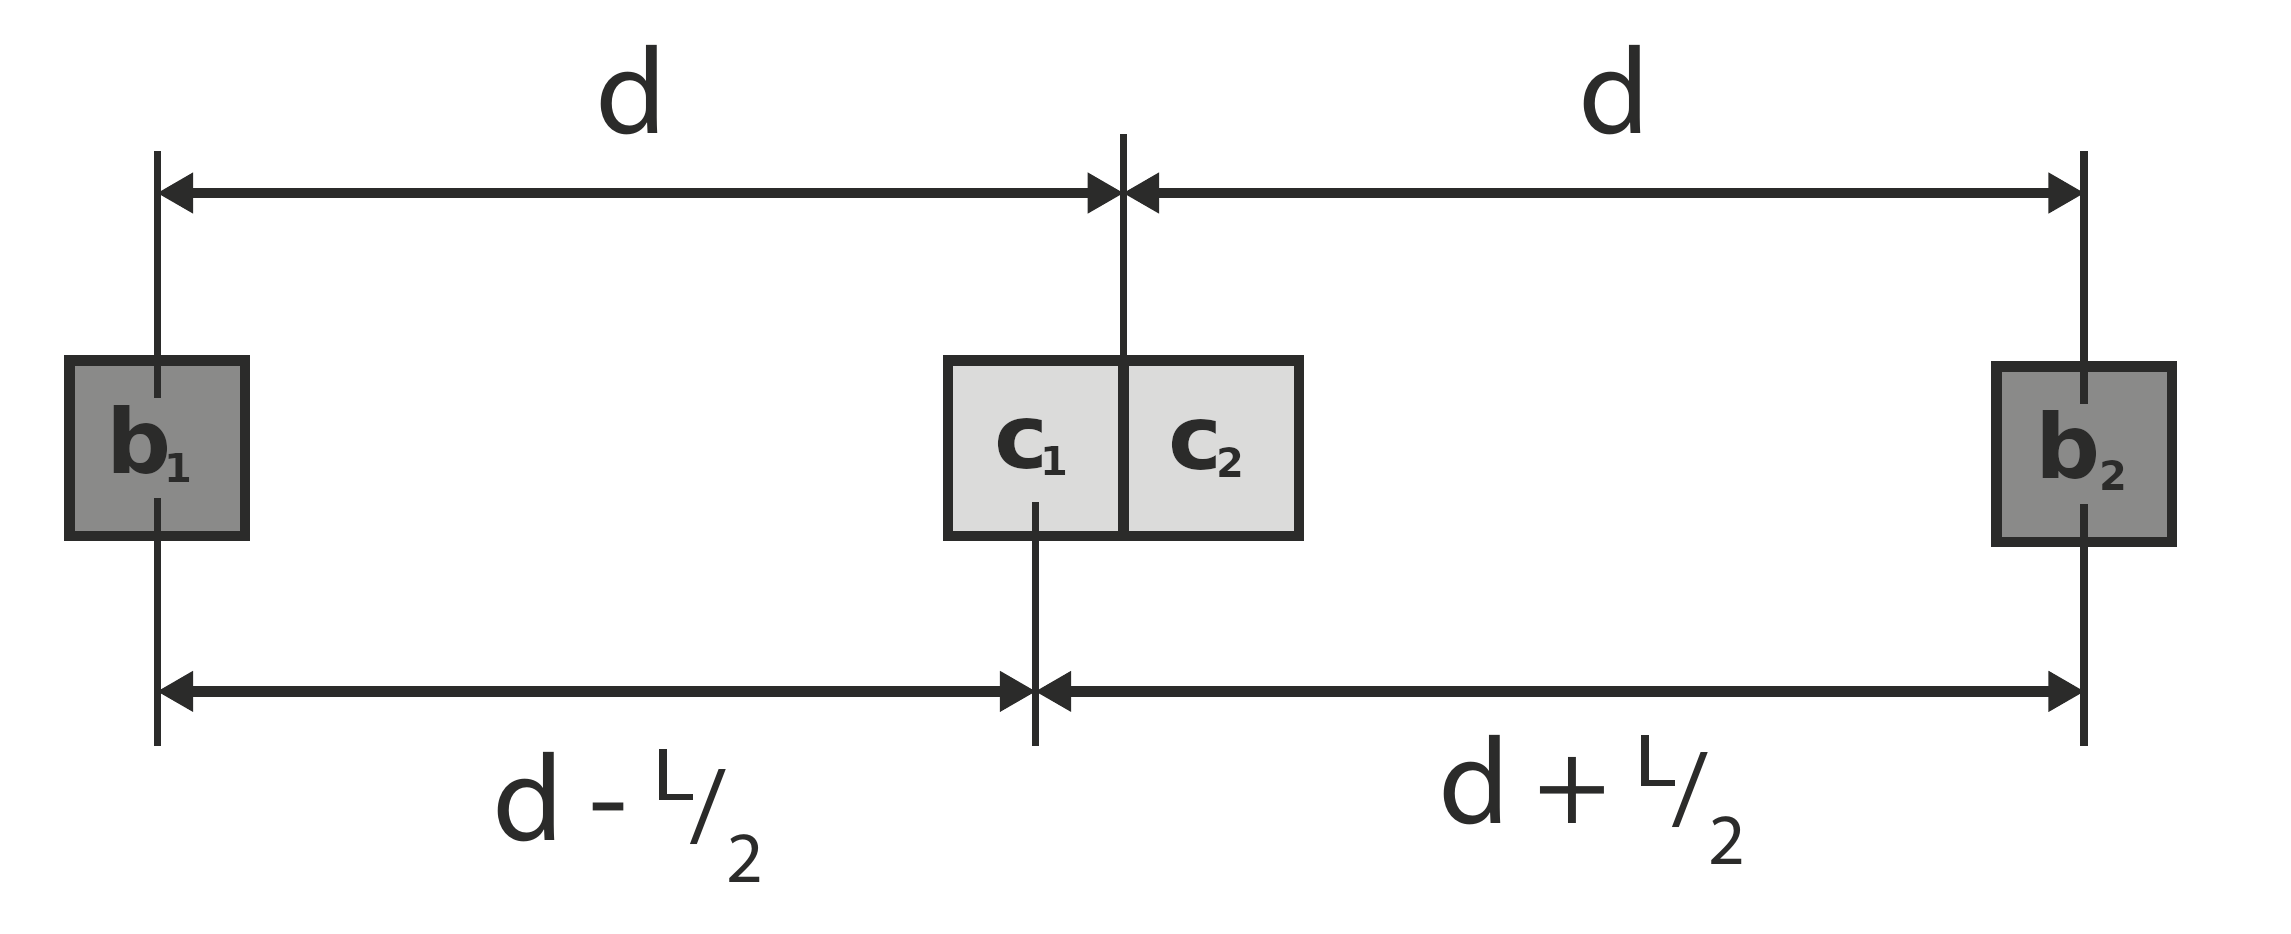
\includegraphics[clip=true, width=0.80\textwidth]{imagenes/basis/horizontalMod.png}

  \caption[Caso en el cual se requiere de una tolerancia para detectar correctmente a las celdas base.]{Caso en el cual se requiere de una tolerancia para detectar correctamente a las celdas base. Modificada de \cite{Liu2015}}\label{fig:bptol}

\end{figure}

La definición presentada en (\ref{eq:bpDisc}) se basa en el análisis realizado
en \cite{Liu2015} donde se resuelve que la tolerancia adecuada entre las
distancias de puntos bases es $L$.

% Con el motivo de incluir celdas como $b_2$ que por
% causa de la discretizacion no estan a una minima distancia $DD(c)$ de $c$ en
% $DBP_c$ . 
% Adaptar directamente la definicion de punto base en espacio continuo a celda base en el espacio discreto resulta en que solo
% las celdas que estan a una distanicia $\mli{DD}(c)$ de $c$, son las que estan a
% minima distancia de $c$, estas serían las unicas celdas base de $c$ si se adaptara de
% forma directa la definicion de punto base en espacio continuo. Sin embargo al adaptar
% de forma directa la definicion existen casos donde los resultados difieren de
% los que se obtienen en el espacio continuo. 
% Un ejemplo es caso que se presenta en la figura \ref{fig:bptol} donde se tiene
% una seccion horizontal de un corredor. En el espacio continuo esto genera la
% pertenecia de los puntos del centro del corredor al GVD, donde cada punto $p$
% que pertenece al GVD tiene dos puntos base, uno a cada lado del corredor a
% distancia $d$ de $p$. El problema ocurre cuando la discretizacion de dicho
% corredor resulta en un numero par de celdas libres entre cada celda ocupada
% correspondiente a una pared del corredor, en este caso se tendran dos celdas
% $c_1$ y $c_2$ en el centro del corredor, $c_1$ tiene una celda $b_1 \in CGen$ a
% minima distancia $d_c(b_1) = DD(c) = d-\frac{L}{2}$, mientras que la celda $b_2
% \in CGen$ está en el otro lado del corrdor a distancia $d_c(b_2) =
% d+\frac{L}{2}$, segun lo que ocurre en el espacio continuo esta
% deberia ser tambien una celda base aunque no este a minima distancia de $c$. La
% tolerancia introducida en la definicion presentada en (\ref{eq:bpDisc}) asegura
% la pertenencia de $b_2$ a $CGen$, recordadndo que $b_2\in CGen$ entoces segun
% dicha definicion se tiene que:


 % Debido a la discretizacion  no lleva a buenos resultados ya que la defincion de
% celda base agrega una tolerancia que permite una correcta generacion del GVD
% discretizado, esta tol

% a celda base sería entoces la celdas pertenecientes a un generador tal que su distancia
% , y dado que $minD$ de
% dichas deldas más cercanas a $c$, tambien se incluyen las celdas que estan a $minD+L$

% 1 defino minD 

% 2 expreso la def en paralabra

% 3 eq

% 4 explico la relacion con la variante continua y el porque de la toreancia (dibujito de liu ming)

% (notar que no es relevante saber a que
% generdor pertnece cada punto)
% \todo{explicar
% problemas de dicretizacion (ming-siegwart)}.

Finalmente las \emph{líneas criticas discretizadas} se definen como las líneas
discretizadas \cite{foleyphillips} definidas entre los centros de las celdas
criticas y cada una de sus celdas base discretizados. El conjunto de todas las
celdas pertenecientes a líneas criticas discretizadas se conoce como
$\mli{LCrD}$.

Una vez determinadas las celdas criticas y las líneas criticas discretizadas es
posible obtener la segmentación en regiones topológicas con la aplicación de un
algoritmo de descomposición en componentes conexas (sección
\ref{subsec:CompComp}) donde el conjunto que se descompone (la entrada del
algoritmo) es el que esta compuesto por las celdas libres de $\mli{CG}$ que no son
celdas criticas ni forman parte de una línea critica discretizada, es decir: 
\begin{align*}
C := \{ c \in \mli{CG} : estado(c) = libre, c \notin \mli{CCr}, c \notin{LCrD}\}
\end{align*}

En la figura \ref{fig:ejSegGVDGrid} se muestra el proceso de segmentación
completo, desde la grilla de ocupación usada como entrada
\ref{fig:ejSegGVDGrid:GRID}, pasando por el GVD generado
\ref{fig:ejSegGVDGrid:GVD}, la detección de celdas criticas y líneas criticas discretizadas
\ref{fig:ejSegGVDGrid:CRI}, terminando con la segmentación del entorno
\ref{fig:ejSegGVDGrid:SEG}.

\begin{figure}[H]
  \centerfloat

  \subfloat[Grilla de ocupacion]{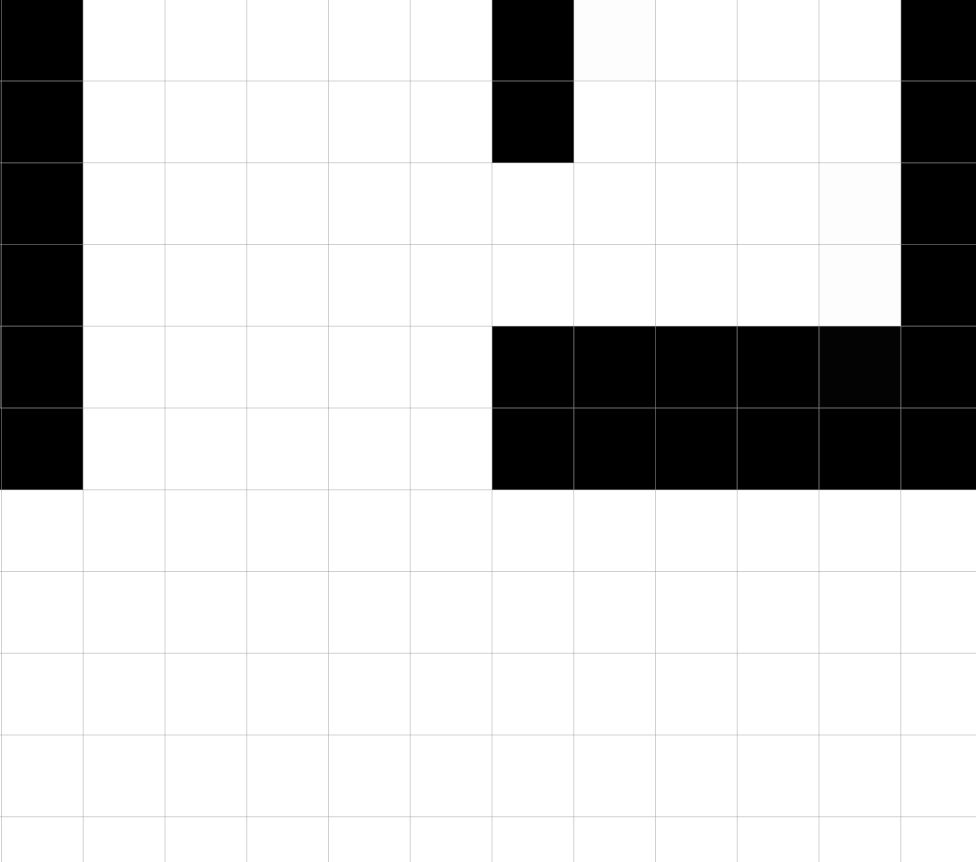
\includegraphics[clip=true,
  width=0.40\textwidth]{imagenes/GVDDisc/a.png}\label{fig:ejSegGVDGrid:GRID}}
  \qquad
  \subfloat[GVD]{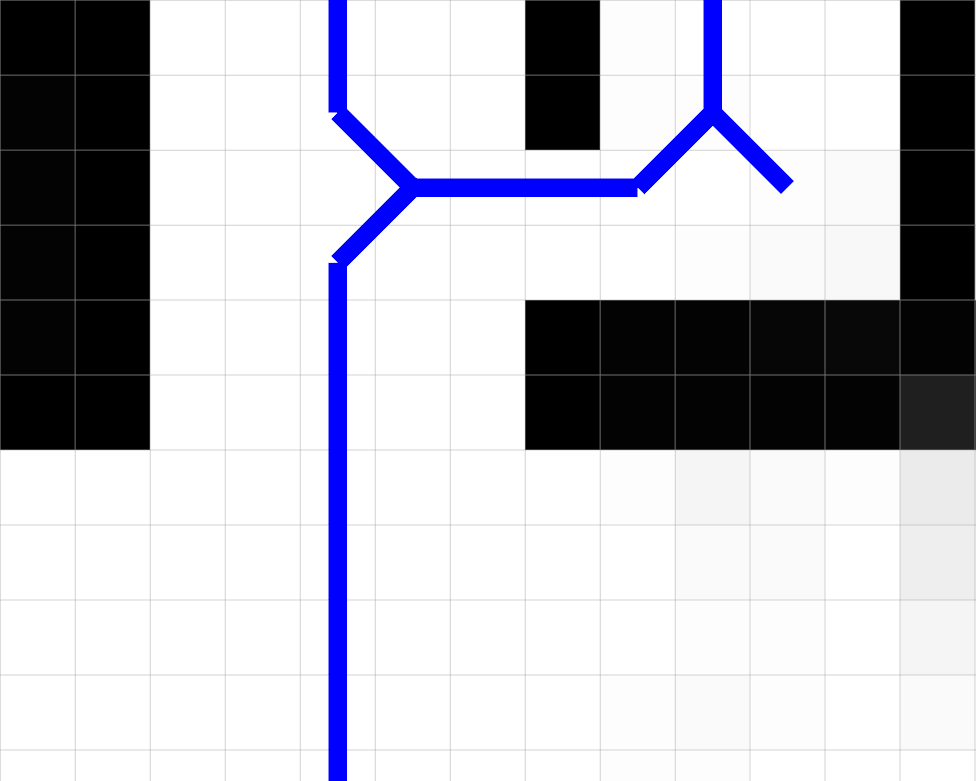
\includegraphics[clip=true,
  width=0.40\textwidth]{imagenes/GVDDisc/b.png}\label{fig:ejSegGVDGrid:GVD}}

  \subfloat[Celdas criticas contienen cuadrados amarillos y las pertinentes a líneas criticas discretizadas contienen cuadrados grises]{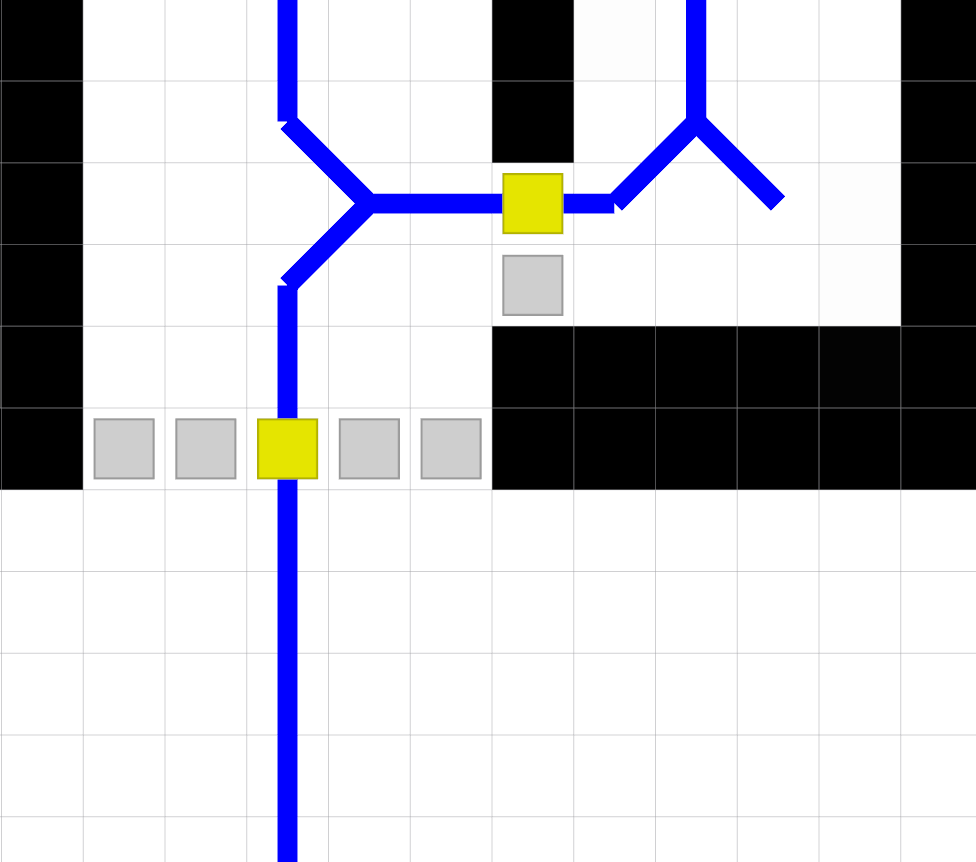
\includegraphics[clip=true, width=0.40\textwidth]{imagenes/GVDDisc/c.png}\label{fig:ejSegGVDGrid:CRI}}
  \qquad
  \subfloat[Segmentación del entorno, cada segmento se indica con un
  color distinto]{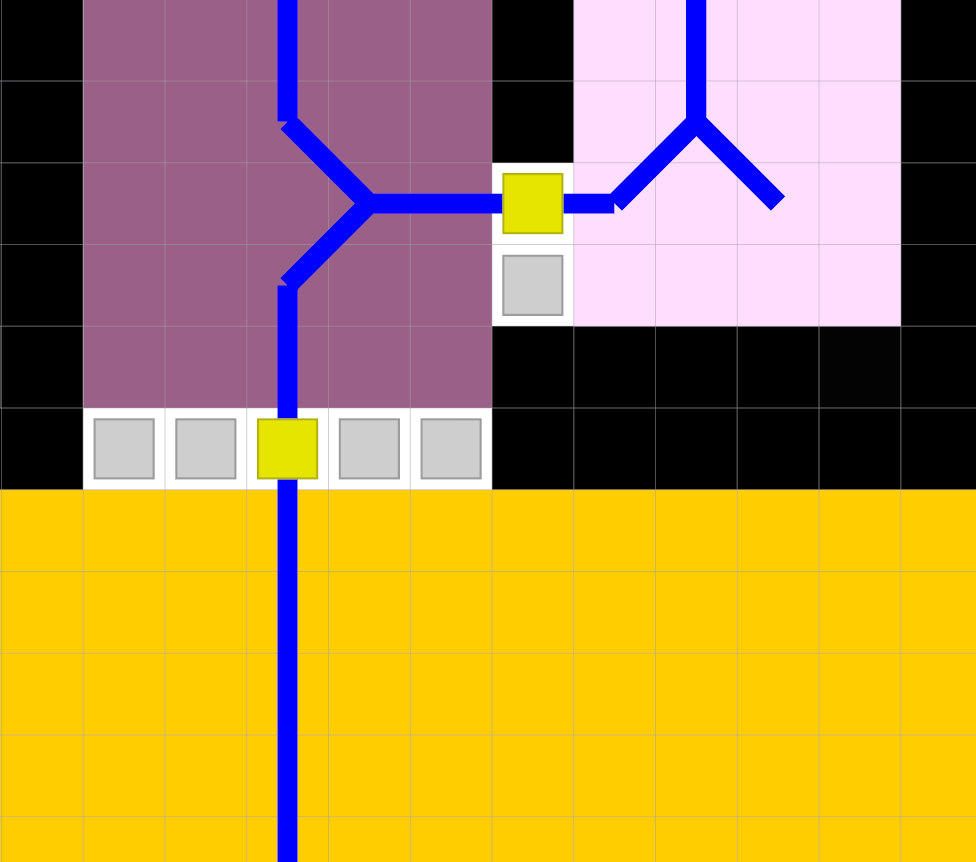
\includegraphics[clip=true,
  width=0.40\textwidth]{imagenes/GVDDisc/d.png}\label{fig:ejSegGVDGrid:SEG}}

  \caption{Proceso de segmentación de un entorno representado con una grilla.}\label{fig:ejSegGVDGrid}

\end{figure}


Una consideración a tener en cuenta es que el algoritmo \ref{alg:compcon} debe
ejecutarse con $ady_4$ como función de adyacencia (sección
\ref{subsec:Grilla}), ya que si se usa $ady_8$ las líneas criticas
discretizadas diagonales no separan segmentos. Esto se debe a que las celdas a ambos lados de una línea
discretizada diagonal son adyacentes diagonalmente como se muestra en la figura
\ref{fig:probDiagSeg}, por lo tanto al usar $ady_4$ la línea critica separa dos
componentes conexas al no permitir la adyacencia entre las celdas a sus lados
mientras que usando $ady_8$ si se permite dicha adyacencia con lo cual resulta
en una única componente.

\begin{figure}[H]
  \centerfloat

% , c es adyacente a n3, lo que causa un único segmento.

  \subfloat[Usando $ady_8$]{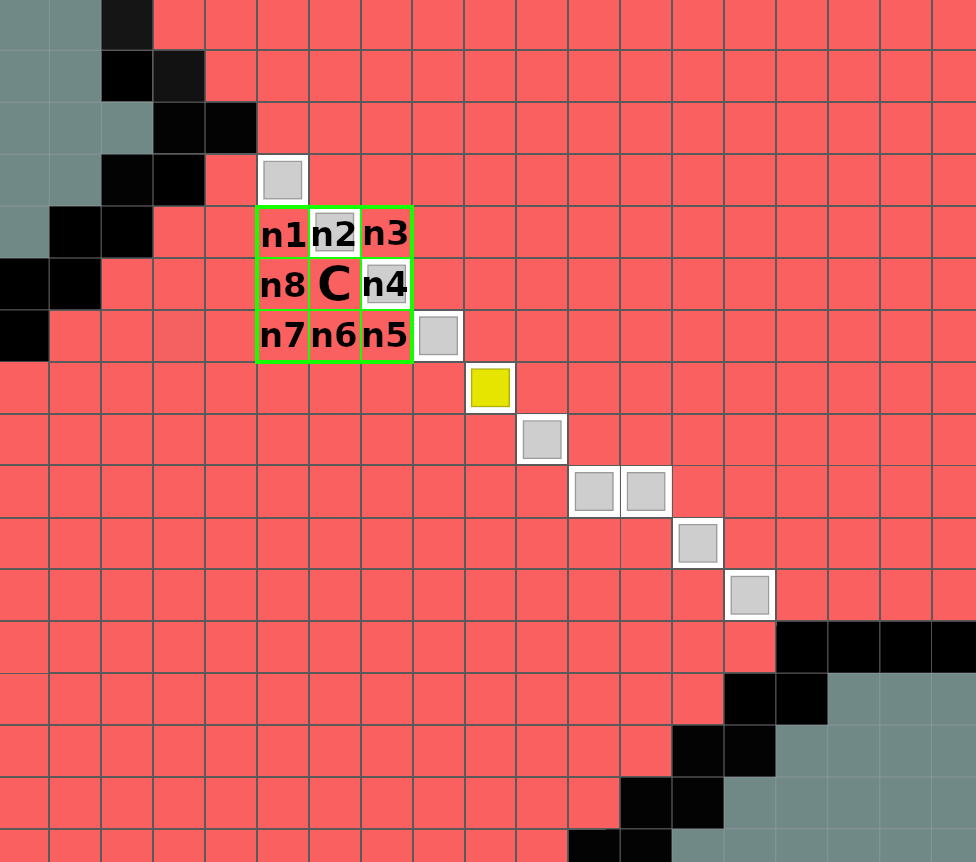
\includegraphics[clip=true, width=0.40\textwidth]{imagenes/probDiagSeg/0_33_8conRojov3.png}}
  \qquad
  \subfloat[Usando $ady_4$]{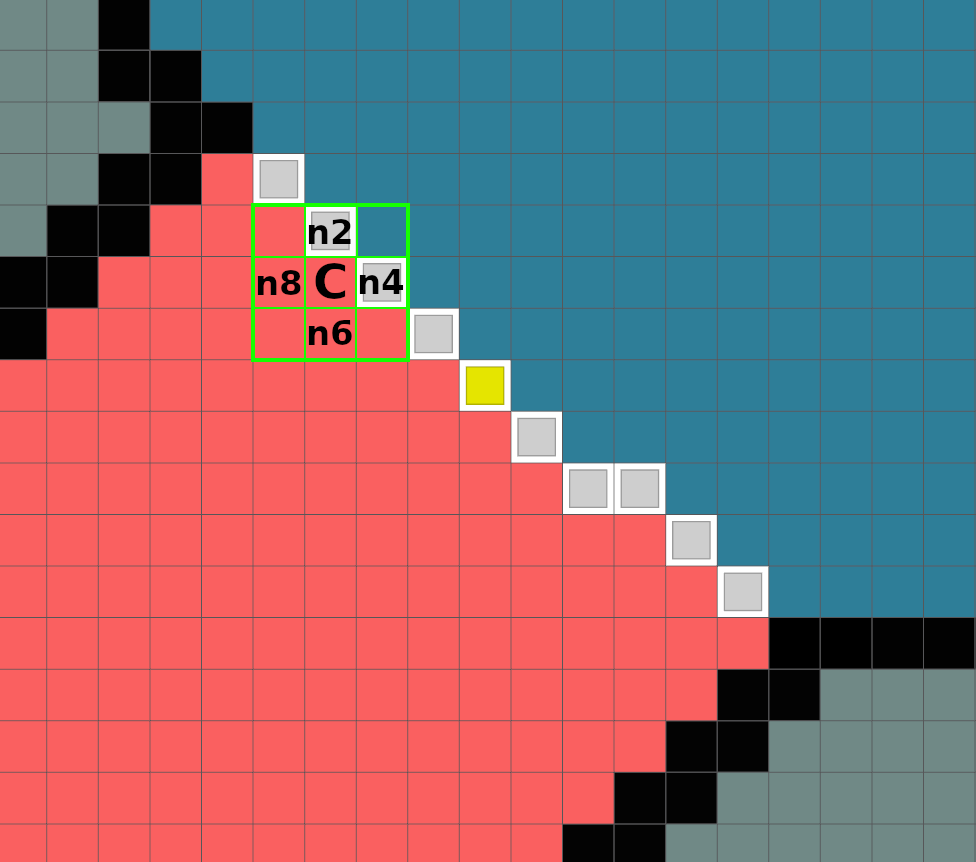
\includegraphics[clip=true, width=0.40\textwidth]{imagenes/probDiagSeg/0_33_4con.png}}

  \caption[línea critica discretizada diagonal, y sus efectos en la
  segmentacion al usar $ady_4$ o $ady_8$.]{línea critica discretizada diagonal, y sus efectos en la
  segmentación al usar $ady_4$ o $ady_8$. La celda $c$ se da como ejemplo de
una celda de un lado de la línea que es adyacente según $ady_8$ a la celda $n3$ al 
otro lado de la línea, cosa que no sucede con $ady_4$.}\label{fig:probDiagSeg}

\end{figure}

% Tambien se filtran las líneas criticas, como las ideas es que estas se ubiquen en umbrales 

% Desribir problemas de desconexion presentados en las diversas implementaciones? 
% \begin{itemize}
%   \item mencionar los de kalra?
%   \item los generados por considerar dist 1 en lau?
%   \item y mostrar que liu ming aunque no explique que hace bien tambien los tiene?
% \end{itemize}

% Aunque existe una etapa de erosion posterior como en Lau para asegurar la
% sparceness. Comentar que se basa en el A de zhang, que en principio es más
% eficiente que chequear patrones

% Se mantienen todos los obts a minima distancia, y los que \say{casi} estan a
% minima distancia, siendo estos los puntos bases (puntos más cercanos a
% generadosres base) tomados en cuenta, segun estos se define si un punto pertenece o no al GVD.



\section{Grafo generalizado de Voronoi}\label{sec:MiConstGVD}

Considerando los problemas de eficiencia del algoritmo no incremental \emph{brushfire} (sección
\ref{subsec:constGVD}) y los problemas de su variante incremental
\emph{brushfire dinámico} (sección \ref{subsec:constGVDInc}) como fue propuesta
originalmente en \cite{kalra2009incremental}, se decidió basar la construcción
del GVD en la version de \emph{brushfire dinámico} propuesta en \cite{Lau2013},
a la que se estará haciendo referencia cuando se mencione \say{\emph{brushfire dinámico}
original} desde este punto.

% (que se
% corresponde con la función de despeje discretizado $\mli{DD} : \mli{CG}
% \rightarrow R$)

La implementación realizada en proyecto mantiene las olas consistentes e
inconsistentes para el calculo incremental de un mapa de distancia.
Adicionalmente mantiene que las olas inconsistentes y consistentes remueven las
celdas que atraviesan del GVD, y que las celdas candidatas a pertenecer al GVD
son las celdas en las que ocurren choques de ondas.

Los cambios principales se dan en el criterio con el cual se determina la
pertenencia de las celdas candidatas al GVD y en como se considera el espacio
desconocido al construir el GVD durante la exploración. Estos se tratan en las
siguientes secciones.

\subsection{Criterio de pertenecía}\label{subsec:critPer}

En \emph{brushfire dinámico} original la pertenecía de las celdas al GVD se
determina en los choques de ondas consistentes. Dada la función $\mli{gen} :
\mli{CG} \rightarrow \mli{CGen}$ que dada una celda $c$ de la grilla devuelve
una de las celdas a minima distancia de $c$ que pertenecen a un generador, el
criterio esencialmente consiste en que, sean $c_1$ y $c_2$ las celdas
involucradas en un choque de ondas consistentes, estas pertenecen al GVD si
$\mli{gen}(c_1) \neq \mli{gen}(c_2)$ y $\mli{gen}(c_1) \notin
ady(\mli{gen}(c_2))$, es decir si $\mli{gen}(c_1)$ y $\mli{gen}(c_2)$ no son
iguales ni adyacentes entre sí. 

La definición de GVD para el espacio continuo donde un punto $p$ pertenece al
GVD si tiene dos generadores distintos a minima distancia, lo cual sucede si y solo si
$p$ tiene al menos un punto a una misma minima distancia en cada uno de esos generadores,
dichos puntos son parte de los puntos base de $p$ (sección
\ref{subsec:mapaTopGVDGrid}). Dado esto que se puede decir que un punto pertenece
al GVD si tiene al menos dos puntos bases que pertenecen a generadores
distintos, lo cual en un espacio discretizado en celdas se traduce a que
existan dos celdas base que pertenecen a generadores distintos.

Dado este análisis y la necesidad de determinar las celdas base planteada en la
sección \ref{subsec:mapaTopGVDGrid}, se determinó diferir en el criterio
pertenencia con respecto al \emph{brushfire dinámico} original, siendo el nuevo
criterio de pertenencia de una celda $c$ al GVD la existencia de dos celdas
base de $c$ pertenecientes a generadores distintos.

La forma de obtener las celdas base de un punto se basa en el concepto de
choque de olas, de forma similar al criterio de pertenencia de celdas al GVD en
el \emph{brushfire dinámico} original. Durante el calculo del mapa de distancia
correspondiente a incremento se registran todas las celdas en involucradas en
choques de olas consistentes. Luego de finalizar la actualización del mapa de
distancia, se obtienen las celdas base $\mli{CB}_c$ de cada celda $c$
registrada previamente según el algoritmo \ref{alg:celdasBase}, notar que la
función de despeje discretizada $\mli{DD} : \mli{CG} \rightarrow R$ se
corresponde los valores del mapa de distancia calculado.

\begin{algorithm}[H]
\SetAlgoLined
  \SetKwInOut{Input}{Entrada}
  \Input{$c$}

% En updateBase c es pN y cA es p
% En setPseudoSourcesFromWave c es p y cA es waveP

  $\mli{minD} := \infty$

  % \tcp{DFS desde $c$ agregando las celdas visitadas a la componente conexa $C_i$}
  \ForEach{ $cA \in ady(c)$} {
    $b := \mli{gen}(cA)$\\
    $\mli{tolerado} := d_c(b) - \mli{DD}(c) \leq L$\\
    $\mli{noIgNiAdy} := b \neq gen(c) \land b \notin ady(gen(c))$\\
    $\mli{masCercano} := d_c(b) < minD$\\
    \If{$\mli{tolerado} \land \mli{noIgNiAdy} \land \mli{masCercano}$}{
      $\mli{minD}  := d_c(b)$\\
      $\mli{minDB} := b$\\
    }
  }
  $\mli{CB}_c := \{\mli{gen}(A)\}$\\
  \If{$\mli{minD} < \infty$}{
    $\mli{CB}_c := \mli{CB}_c \cup \{\mli{minB}\}$\\
  }
  \Return $\mli{CB}_c$ 

  \caption{Obtención de las celdas base $\mli{CB}_c$ de la celda $c$ (simplificada)}
  \label{alg:celdasBase}
\end{algorithm}

El algoritmo procesa cada celda $cA$ adyacente a $c$ (línea 2) obteniendo el
candidato a ser una celda base de $c$ (línea 3) y comprobando una serie de
condiciones para que este candidato pueda ser una celda base de $c$ (líneas
4-6). La condición que se comprueba en la línea 4 es que el punto base
candidato este dentro del intervalo definido por la tolerancia como fue
definido en la sección \ref{subsec:mapaTopGVDGrid}. En la línea 5 la condición
verifica que el candidato no puede ser la celda perteneciente a un generador
más cercana a $c$ ni adyacente a esta. Finalmente la condición presente en la
línea 6 establece que el candidato actual debe tener una distancia a $c$ menor
que la de los candidatos procesados anteriormente que cumplen el resto de las
condiciones. Al finalizar la ejecución se devuelve como celdas bases a la celda
perteneciente a un generador que es cercana a $c$ y en el caso de que exista al
ultimo candidato en cumplir todas las condiciones (líneas 12-16).

%(sacr de la implementacion) (notar que gens a igual distancia tambien se encuentran, igual no comentar por las dudas)

% Notar el uso de la tolerancia de un largo de celda determinada en \cite{Liu2015}

Habiendo obtenido las celdas base de un celda $c$ para determinar la
pertenencia de $c$ al GVD resta verificar si existen al menos dos celdas base
que pertenecen distintos generadores. Para esto se aplica una técnica derivada
del criterio de pertenencia de celdas al GVD presente en el \emph{brushfire dinámico}
original, que consiste en que dos celdas distintas y no adyacentes entre
sí pertenecen a distintos generadores, y de lo contrario pertenecen al mismo
generador. De esta forma se logra aproximar el GVD resultante de considerar
generadores conexos y convexos \ref{subsec:GVD} sin definir explícitamente los
generadores. Y adicionalmente se obtienen las celdas base a partir necesarias
para segmentar.

Es pertinente aclarar que el algoritmo \ref{alg:celdasBase} es una version
simplificada del que esta presente en la implementación del proyecto. Las
simplificaciones son dos, la primera es que se considera solo una de las celdas
a minima distancia que pertenecen a un generador (la devuelta por la función
$gen$), similar a como se trabaja en el \emph{brushfire dinámico} original. La
segunda es que solo se permiten dos celdas base. En la sección
\ref{algComp:celdasbase} se presenta el algoritmo completo para obtener las
celdas base sin las simplificaciones mencionadas, es decir que maneja todas las
celdas pertenecientes a generadores que están a minima distancia y permite más
de dos celdas base.

\subsection{Consideraciones sobre el espacio desconocido}\label{subsec:espDesc}

Durante la exploración existe un conjunto de celdas de estado desconocido en la
grilla de ocupación (sección \ref{subsec:Grilla}) usada para representar el
entorno explorado, dichas celdas representan la existencia de porciones del
entorno sin explorar. Dado que la definición del GVD no contempla el espacio
desconocido, para poder construir un GVD sobre grillas de ocupación durante la
exploración es necesario tomar una decision acerca de como considerar el 
espacio desconocido. Sin embargo, este no es un tema que se trate de forma
explicita en los trabajos estudiados sobre la construcción incremental de GVD. 

A partir del código e imágenes disponibles es posible deducir que en
\cite{kalra2009incremental} y \cite{Lau2013} al construir el GVD las celdas de
estado desconocido se consideran iguales que las de estado libre. De esta
forma se obtienen resultados similares a los que se presentan en la figura
\ref{fig:kalraOG}. Notar que otra característica particular presente en estas
implementaciones es que las celdas ubicadas en los bordes del entorno se
consideran como pertenecientes a generadores.

\begin{figure}[H]
  \centerfloat

  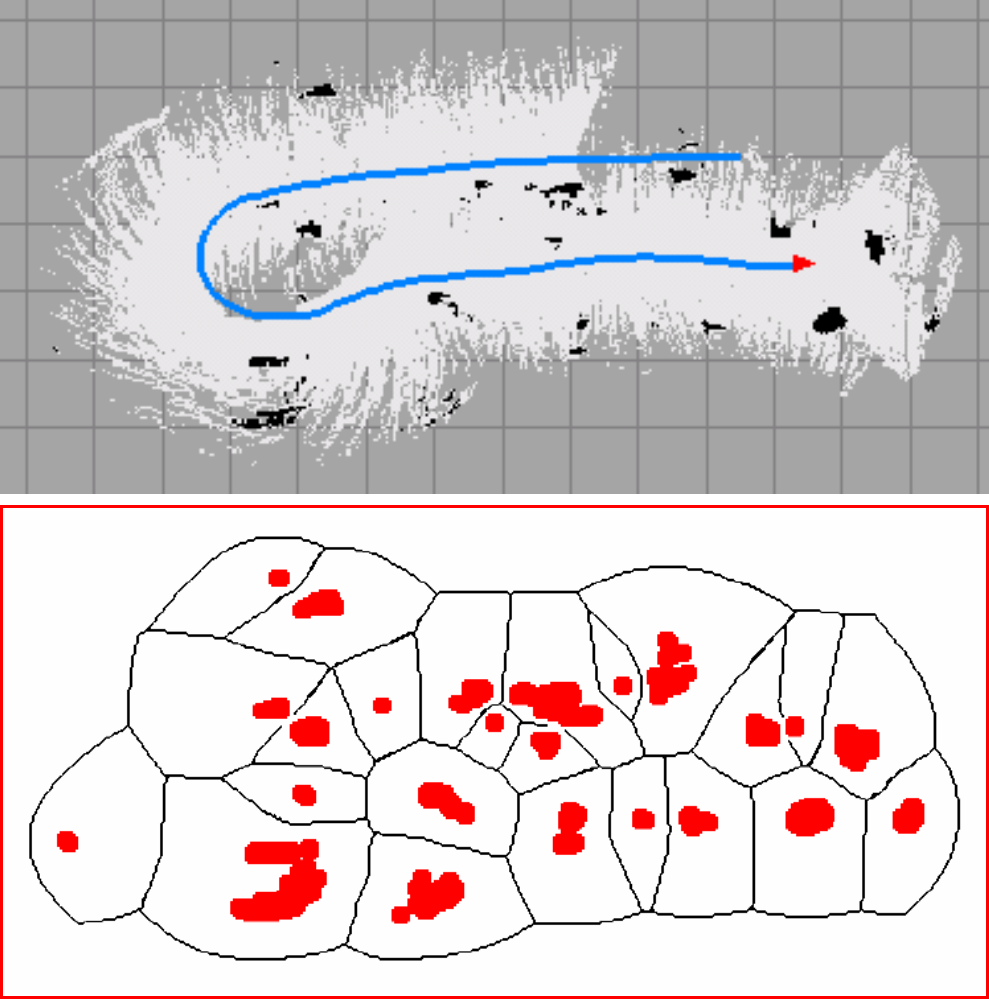
\includegraphics[clip=true, width=0.75\textwidth]{imagenes/desconocidoCons/kalraOG.png}

  \caption[Consideración del espacio desconocido presente en \cite{kalra2009incremental} y \cite{Lau2013}.]{Consideración del espacio desconocido presente en \cite{kalra2009incremental} y \cite{Lau2013}. En la parte superior se muestra la grilla de ocupación actual. En la inferior su GVD correspondiente, indicándose con rojo los obstáculos. Extraída de \cite{kalra2009incremental}.}\label{fig:kalraOG}
\end{figure}

Que las las celdas desconocidas se traten igual que las celdas libres implica
que las olas utilizadas para construir el GVD pueden propagarse por el espacio
desconocido y generar la pertenecía de la celdas desconocidas al GVD, lo cual
tiene asociado un costo computacional.
En la figura \ref{fig:desconocidoKalra} se puede observar como la tratar las
celdas desconocidas como conocidas lleva a un GVD que abarca todo el entorno
sin importar que solo una pequeña porción del espacio sea conocida. 

%mantener un GVD conexo,
% (por motivos que se seran comentados a continuacion)

Dado que en el contexto del proyecto no es necesario construir GVD fuera del
area conocida se desarrollo una técnica que solo construye GVD en las celdas
conocidas evitando trabajar sobre espacio desconocido. Esta consiste en no
permitir que las olas se propaguen por el espacio desconocido, y
adicionalmente considerar al conjunto $\mli{UF}$ de celdas desconocidas que tienen un
vecino conocido como celdas pertenecientes a generadores
($\mli{UF}\subseteq \mli{CGen}$) junto a las celdas ocupadas.
De esta forma para el caso presentado en la figura \ref{fig:desconocidoKalra}
se obtiene un GVD que se reduce al espacio conocido como se muestra en la
figura \ref{fig:desconocidoMio}.
% evitando propagar las olas sobre el espacio desconocido, 

\begin{figure}[H]
  \centerfloat

  \subfloat[Celdas desconocidas se consideran como libres.]{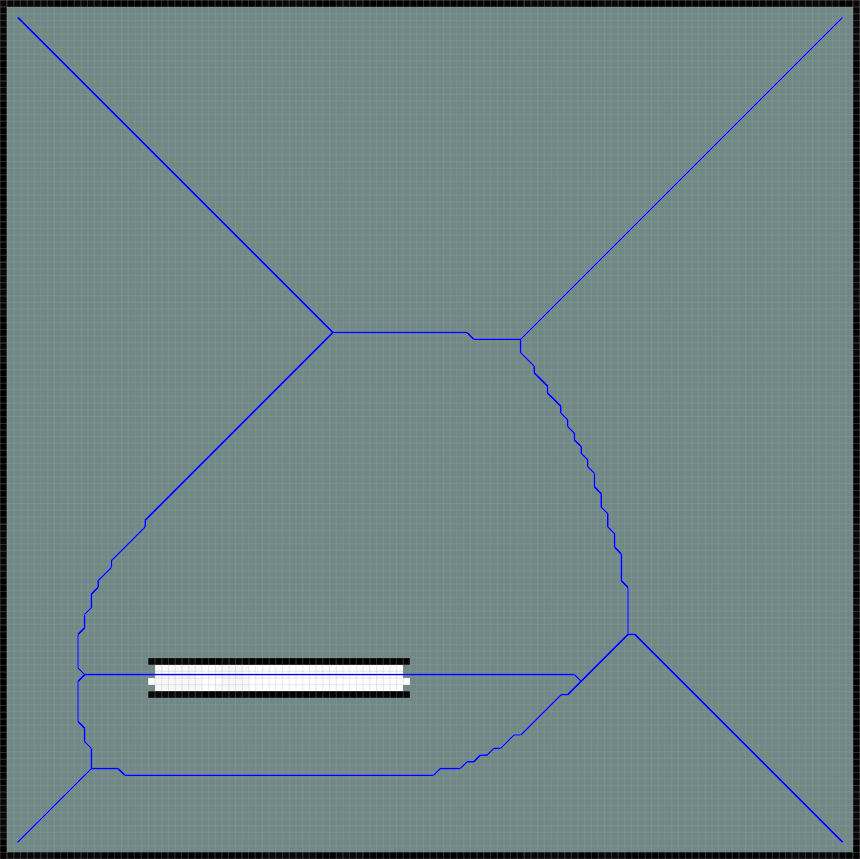
\includegraphics[clip=true, width=0.45\textwidth]{imagenes/conectividad/kalra.png}\label{fig:desconocidoKalra}}
  \quad
  \subfloat[Celdas desconocidas no propagan ondas y $\mli{UF}\subseteq \mli{CGen}$.]{
\includegraphics[clip=true, width=0.45\textwidth]{imagenes/conectividad/mio.png}\label{fig:desconocidoMio}}

  \caption[Formas de considerar el espacio desconocido.]{Formas de considerar el espacio desconocido. El GVD generado se indica en azul.}\label{fig:desconocidoEj1}
\end{figure}


El solo considerar que las celdas desconocidas no propagan ondas tiene el
problema de resultar en GVD disconexos en casos donde esto se puede evitar. El
problema con los GVD disconexos es que estos no cumplen con la propiedad de
\emph{conectividad} necesaria para ser un \emph{roadmap} (sección
\ref{subsec:mapacarr}), lo cual genera errores de usarse el GVD como
\emph{roadmap} para la planificación. En la figura \ref{fig:desconocidoEj2} se
muestra el GVD generado en una misma grilla de ocupación con cada una de las
tres formas de considerar el espacio desconocido mencionadas, es posible
observar que el GVD resultante de solo considerar que las celdas desconocidas
no propagan ondas no preserva la conectividad, mientras que los otros dos
métodos otros si lo hacen.

% El problema presentado por esta forma de considerar el espacio desconocido es
% que las ondas se propagan por el espacio desconocido, generado GVD fuera del

% al explorar donde en un mapa no solo hay obtaculos y celdas libres si no que tambien hay celdas desconocidas,
% Llamado de atencion al problema de conectividad de un GVD al explorar donde en un mapa no solo hay obtaculos y celdas libres si no que tambien hay celdas desconocidas, las cuales no se consideran en los articulos del estado del arte. Estos se asume (no se explicita pero en Kalra se ve que el mapa para entorno abierto es consistente con esta tecnica, en el codigo de lau tambien) que implementan la tecnica de "los limites de mi mapa son obstaculos" y lo desconocido es libre. En este trabajo se propone una tecnica novedosa que soluciona este problema de forma más eficiente evitando procesar todo el espacio desconocido mientras se va explorando.

\begin{figure}[H]
  \centerfloat

  \subfloat[Celdas desconocidas se consideran como libres.]{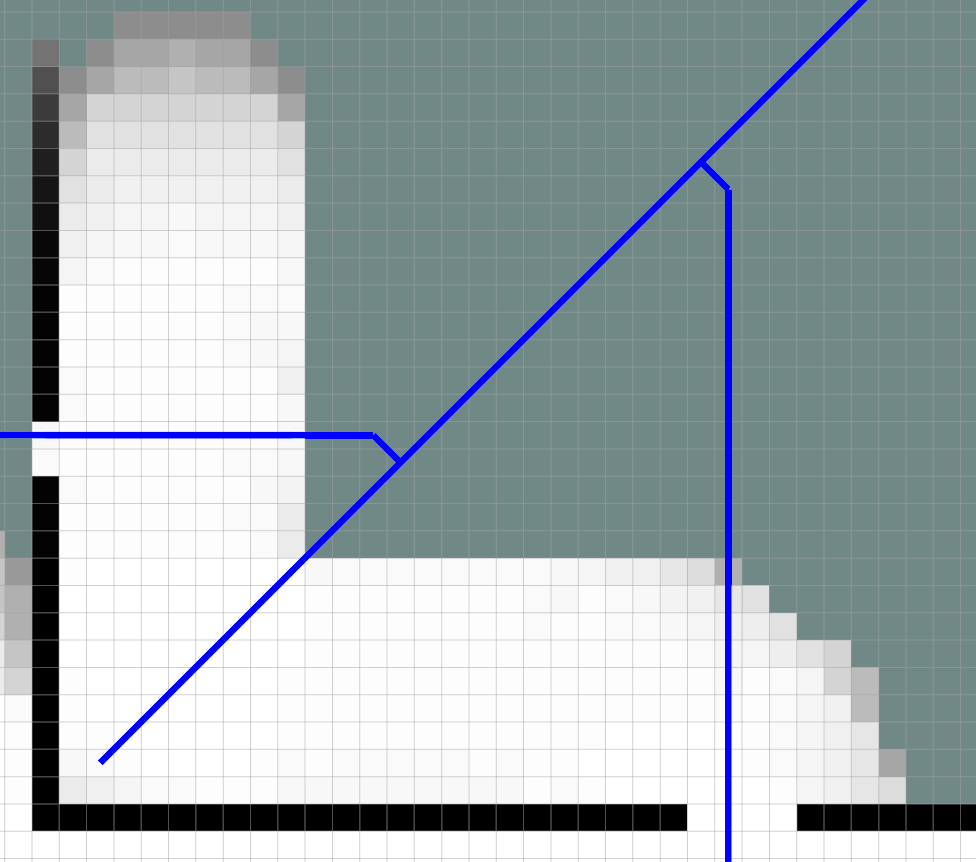
\includegraphics[clip=true, width=0.32\textwidth]{imagenes/desconocidoCons/kalra.png}}
  \quad
  \subfloat[Celdas desconocidas no propagan ondas y $\mli{UF}\subseteq \mli{CGen}$.]{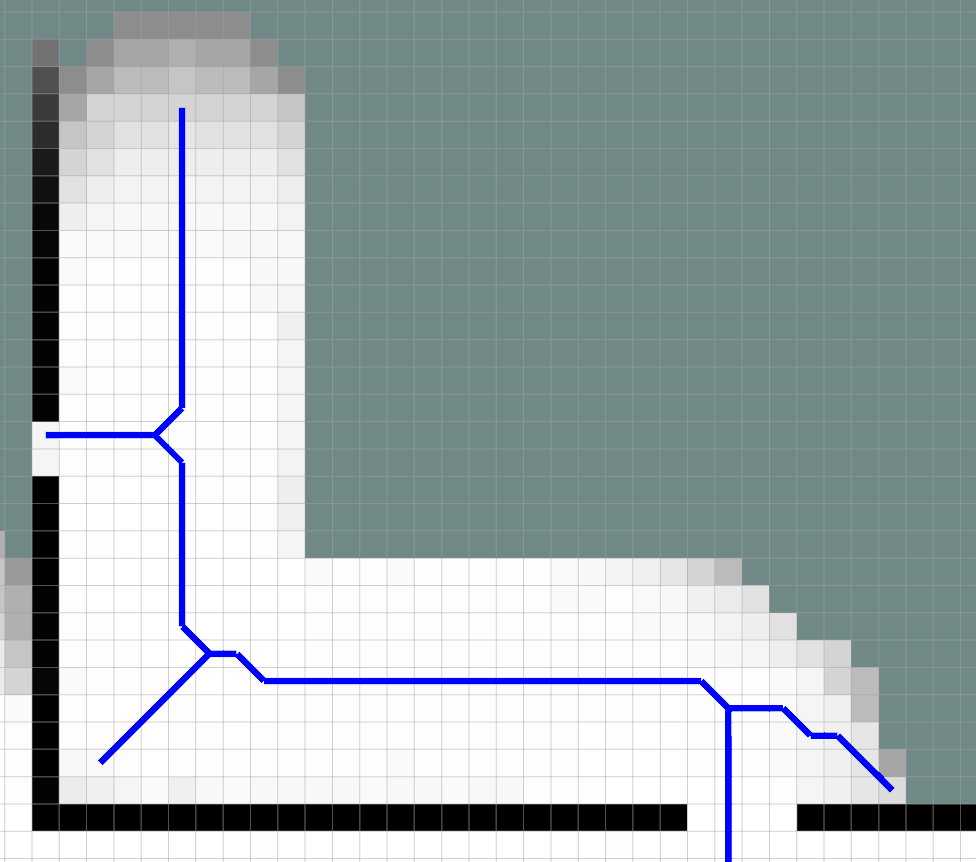
\includegraphics[clip=true, width=0.32\textwidth]{imagenes/desconocidoCons/mio.png}}
  \quad
  \subfloat[Celdas desconocidas no propagan ondas.]{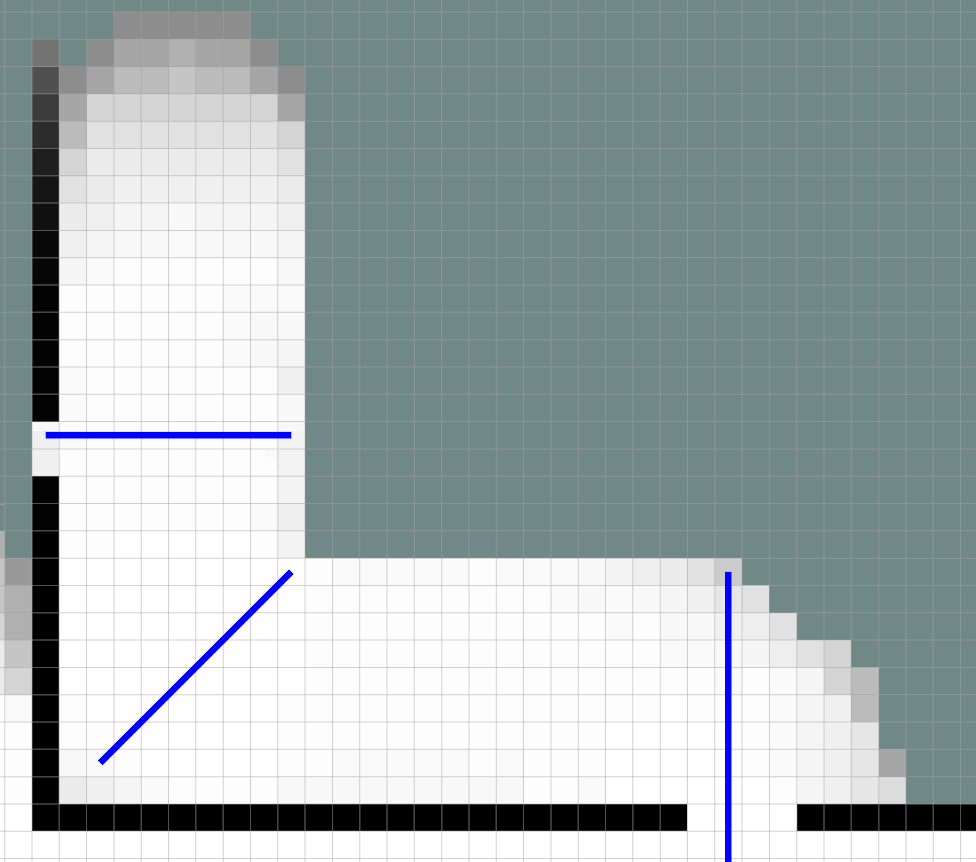
\includegraphics[clip=true, width=0.32\textwidth]{imagenes/desconocidoCons/noHacerNada.png} \label{fig:desconocidoEj2_naive}}

  \caption[Conectividad en diferentes formas de considerar el espacio desconocido.]{Conectividad en diferentes formas de considerar el espacio desconocido. El GVD generado se indica en azul.}\label{fig:desconocidoEj2}
\end{figure}

% 1. desconexiones
% 2. incrementalmente si se agregan celdas libres que no son obstaulos entonces igual es necesario actualizar el GVD

% , la alternativa de que los bordes no sean
% Obstaculos (como esta no aplica a entornos abiertos y genera más costos) y


% Explicar el problema de considerar lo desconocido, como no hacerlo lleva a GVD
% disconexos, explicar lo que se encuentra en el estado del arte (explicar como
% esta aplica para entornos abiertos) y la alternativa de que las fronteras
% (invertidas) sean emisoras de ondas consistentes e inconsistentes y lo
% desconocido no sea atravezable por las ondas y porque esto implica mucho menos
% costos para mapas cuando estos se comienzan a explorar y se componen de muchas
% celdas desconocidas.

% Comentar que las celdas con lo desconocido como punto base no genera líneas ni
% puntos criticos.

% \todo{FEDE: Kalra se ve que el mapa para entorno abierto es consistente con esta tecnica, en el codigo de lau tambien. Pero no se hace referancia a esto}

% Mostrar gvd resultantes de mapas parcialemnte explorados (muy poco explorados) y comentar como toda el area desconocida debe ser procesado por el original mientras que el mio se reduce al area exploradoa, sientod la parte importante (la del area explorada) casi igual que la otra.

\section{Planificación}\label{sec:miNav}
% Recordando que el camino consiste en una secuencia puntos en el espacio, en el
% contexto de la planificación estos se denominan como subobjetivos con exepcion
% del ultimo punto llamado como objetivo.

% En el contexto de la planificación los puntos que componen el
% camino se denominan subobjetivos con exepcion del ultimo punto que se denomina
% como objetivo.

Una vez que el robot recibe un objetivo de exploración, desde la central
(sección \ref{sec:asigTar}), el robot debe moverse físicamente hasta el lugar
indicado para completar dicho objetivo y progresar en la exploración del entorno.

El modulo encargado de recibir el objetivo es el \emph{controlador del robot},
este tiene la tarea de recuperar de la memoria del robot el camino que fue
determinado durante la valuación de dicho objetivo (sección
\ref{subsec:MiValSub}) y transmitir dicho camino al modulo \emph{controlador de
movimiento}. 

% Una que el caminno llega al modulo \emph{controlador de movimiento}
% trabaja
% junto al modulo \emph{move base} para lograr su comentido.

 % puntos
% del camino, son relevantes para poder llegar al objetivo.

% que se
% considera no completado al modulo \emph{move base} el cual se encarga de
% generar las directivas a los motores del robot para que pueda llegar de forma
% segura a dicho objetivo/subobjetivo.

% Para determinar que punto debe ser enviado a
% \emph{move base} el \emph{controlador de moviemiento} 

% Adicionalmente tiene la tarea de determinar cuando un punto
% se considera completado

% Especificamente el \emph{controlador de
% moviemiento} comienza enviando el primer punto del camino  En algun punto de la trayectoria hacia el
% objetivo/subobjetivo que lleva a cabo \emph{move base} este se considera
% completado, dado esto el siguiente objetivo/subobjetivo sin completar se envia
% a \emph{move base}. El proceso se repite hasta completar el objetivo,
% completando asi el camnino completo.

El modulo \emph{controlador de movimiento} se encarga de enviar puntos del
camino al modulo \emph{move base} que genera las directivas necesarias para que
el robot avance hacia dicho punto. Estos puntos deben enviarse en una secuencia
que permita que el robot puede seguir el camino hasta el objetivo. Para lograr
esto asumiendo que se tiene un criterio que permite considerar cuando un punto del camino se
considera completado, el funcionamiento del \emph{controlador de
movimiento} consiste en determinar el primer punto no completado del camino
asignado, enviar dicho punto a \emph{move base} y esperar a que el robot avance
lo suficiente para completarlo. Una vez completado se repite el
proceso con el siguiente punto sin completar, esto sucede hasta que se completa
el ultimo punto del camino, el objetivo.

% Para determinar cuando un punto del camino considera completado, estos se separan  el ultimo punto  objetivo  subobjetivos con exepcion del ultimo punto que se denomina
% como objetivo.

\subsection{Criterios de compleción}

El \emph{controlador de movimiento} tiene dos formas de considerar completo un
punto del camino, la normal y la forzosa.

La compleción forzosa ocurre cuando el robot esta a una distancia menor que
$\mli{DistF}$ del punto en cuestión. Este criterio de compleción tiene como
propósito determinar cuando un robot esta lo suficientemente cerca de un
punto del camino como para considerarlo completo a pesar de que no se dio
aun la compleción normal. Siendo el valor de $\mli{DistF}$ establecido para
cumplir con el propósito de la compleción forzosa, para esto debe considerarse
las principalmente las dimensiones del robot.

Por otro lado para la compleción normal existen dos condiciones, la primera es
que exista una línea de ancho $Seg$ entre el robot y el punto del camino que al
discretizarse en celdas no contiene ninguna ocupada. La segunda, en el caso del
ultimo punto del camino (el objetivo) la distancia en entre este y el robot
debe ser menor a $\mli{DistNo}$, en el resto de los puntos (subobjetivos) la distancia debe
ser menor a $\mli{DistNs}$.

El valor $\mli{DistNo}$ debe cumplir con
$\mli{DistF}<\mli{DistNo}<\mli{rango}$, siendo $\mli{rango}$ el alcance de los
sensores del robot. Esto se debe a que la idea detrás de criterio de compleción
normal aplicado al objetivo es considerarlo completo cuando es seguro que dicho objetivo
esta en el rango de sensado del robot. Esto implica que el robot esta en
condiciones de recopilar nueva información del entorno, siendo este el motivo
por el cual el objetivo fue asignado en un primer lugar.

El valor $\mli{DistNs}$ solo debe ser mayor que $\mli{DistF}$, y establece que
tan estrictamente se sigue el camino original en espacios despejados de
obstáculos. Valores pequeños de $\mli{DistNs}$ hacen que el robot siga el
camino original de forma estricta aunque este en espacios despejados ya que se 
fuerza que el robot este cerca de los subobjetivos para completarlos. Al
aumentar el valor de $\mli{DistNs}$ se permite mayor libertad en como seguir el
camino original cuando el espacio esta despejado, esto sucede porque en los
espacios despejados todos los subobjetivos del camino que estén a una
distancia menor a $\mli{DistNs}$ se consideran completados, siendo move base el
encargado de la trayectoria hasta el primer punto no completado del camino,
sin ser necesario pasar cerca por los subobjetivos previamente completados.

\subsection{Planificación jerárquica}
% es que los caminos originales
% calculados sobre el GVD (seccion \ref{subsec:MiValSub})
Los GVD son estructuras que se representan con un cantidad considerablemente
menor de celdas que las presentes la grilla de ocupación a partir de la cual son
generados. A pesar de esto, los GVD son \emph{roadmaps} (sección
\ref{subsec:mapacarr}) por lo que permiten planificar caminos entre cualquier par de
puntos del espacio, al igual que las grillas de ocupación. 

La diferencia de tamaños implica que los caminos generados sobre el GVD tienen
una menor en costo computacional que los calculados sobre la grillas de
ocupación. Pero a su vez, los caminos generados sobre el GVD se encuentran lo
más alejado posible de los obstáculos (sección \ref{subsec:GVD}), lo que lleva a
caminos que aunque son seguros, pueden resultar innecesariamente largos.

La motivación de la planificación jerárquica es aprovechar la eficiencia de los
caminos generados sobre el GVD, evitando los desvíos innecesarios que estos
contienen.

La planificación jerárquica consiste en utilizar la información
topológica del camino generado del GVD, específicamente se utilizan los
puntos del camino que se encuentran en las transiciones entre los
segmentos (habitaciones y corredores) para establecer un camino de alto
nivel compuesto por la secuencia de estos puntos y el objetivo final.
Luego caminos de bajo nivel se establecen entre el robot y el siguiente
punto del camino de alto nivel, la idea de estos caminos es que el robot
pueda navegar libremente (sin considerar el GVD) dentro de los
segmentos, moviéndose de transición en transición. La planificación de
los caminos de bajo nivel se delega a \emph{move base}, el cual genera
caminos sin desvíos innecesarios.

Es pertinente notar que en la implementación realizada \emph{move base} se
configuro con un planificador global que calcula caminos sobre la grilla de
ocupación (sección \ref{subsec:move_base}), de igual manera aplicar esta
técnica simplifica los cálculos de caminos sobre la grilla siendo dichos
cálculos locales a cada segmento que se debe transitar.

Esta planificación jerárquica se lleva a cabo estableciendo un valor de
$\mli{DistNs}$ mayor a las dimensiones de los segmentos y un valor de
$\mli{Seg}$ mayor al tamaño de los portales de transición entre
segmentos (puertas, pasajes abiertos). De esta forma asumiendo segmentos
despejados, todos los subobjetivos asociados a un segmento en el que se
encuentra un robot son completados de forma normal. Por lo tanto en en
caminos largos que abarcan varios segmentos, los únicos subobjetivos
enviados a \emph{move base} son los que se ubican en las portales entre
un segmento y el siguiente en el camino, los cuales no son completados
de forma normal ya que dicha transición consiste en un portal de ancho
menor a $\mli{Seg}$ que no permite la existencia de una línea
discretizada de ancho $\mli{Seg}$ que no contenga obstáculos.

En la figura \ref{fig:navjer} se muestra un ejemplo en el cual se puede
apreciar la diferencia de largos entre el camino original ubicado sobre
el GVD y el de bajo nivel que lleva hacia la celda ubicada sobre el
portal en la transición al siguiente segmento del camino.

\begin{figure}[H]
  \center
  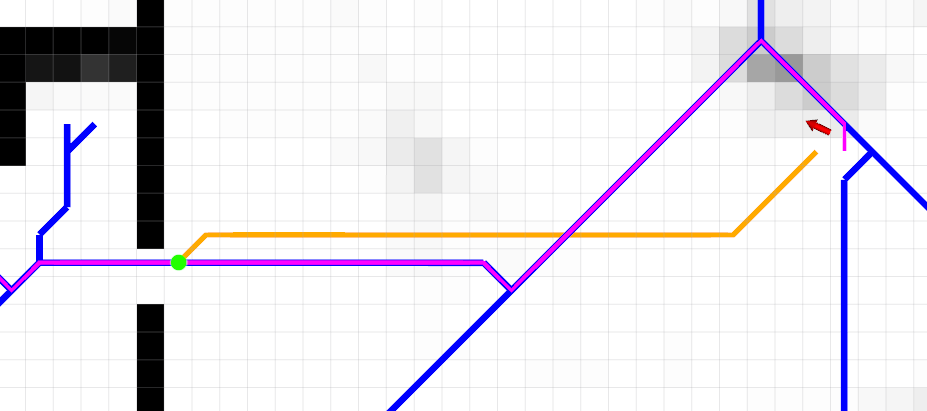
\includegraphics[width=1\linewidth]{imagenes/navjer/caso1/a.png}
  \caption[Planificación jerárquica.]{Planificación jerárquica. El GVD
    se indica con azul. En magenta se marca el camino original y en
    naranja el de bajo nivel, siendo el punto verde el primer
    subobjetivo sin completar del camino original. El vector rojo indica
    la posición y orientación del robot.
 }
  \label{fig:navjer}
\end{figure} 


\section{Construcción cooperativa del mapa}
% Durante la exploración la grilla de ocupación (seccion \ref{subsec:Grilla}) que
% representa el entorno explorado celdas  estado se puede determinar como
% ocupadas, libres y desconocidas

% Para una celda $c$ con estado desconocido, es equiprobable que $c$ este ocupada o 
% libre, siendo necesaria evidencia de
% que la celda esta ocupada ni de que esta libre, para que la celda cambie su
% estado ya sea a libre o a ocupado. En un escenario donde se comienza sin conocimiento sobre
% el entorno explorado y que el objetivo de la exploración es obtener
% informacion de dicho entorno, es posible decir que todas las celdas comienzan con estado desconocio 
% y el numero de celdas en dicho estado decrece a lo largo que transcurre la
% exploración, a medida que se obtiene informacion (evidencia) sobre el entorno.


A lo largo de la exploración los robots de la flota son asignados a objetivos
de exploración, cuando un robot completa un objetivo este sensa porciones del
entorno antes desconocido. Esta nueva información debe ser manejada para
aportar a la construcción de la grilla de ocupación (mapa) con la cual se
representa el entorno explorado. A continuación se describe el proceso completo
desde los sensores hasta la construcción de un mapa que contenga toda la
información obtenida del entorno.

Cada robot esta constantemente recopilando información del entorno a través de
sus sensores y enviando dicha información al nodo de \gls{ROS} \emph{global\_costmap}
ubicado en su modulo \emph{move base} (sección \ref{subsec:move_base}). Al
recibir datos sensoriales \emph{global\_costmap} actualiza la grilla de
ocupación que construye. \emph{Global\_costmap} fue configurado para que los
valores de probabilidad de ocupación asociados a las celdas de su grilla de
(sección \ref{subsec:Grilla}) solo dependan de la ultima evidencia sensorial
obtenida para cada celdas. Adicionalmente las celdas tienen asociado uno de
tres valores de probabilidad de ocupación posibles: $0.5$ indicando que la
celda es desconocida, $0.55$ indicando que la celda esta ocupada y $0.45$
indicando que la celda esta libre. Estos valores indican la probabilidad
$P(c|x_t,z_t)$ de que una celda $c$ este ocupada dada una única medida $z_t$
desde una cierta posición $x_t$.

Dado que cada \emph{global\_costmap} construye una grilla de ocupación solo
considerando los datos sensoriales del robot en el cual ejecuta, estas se deben
combinar en una que centralice toda la información recopilada del entorno. Esto
se logra configurando los \emph{global\_costmap} para que cuando se den
modificaciones en estas grillas se envíen las porciones modificadas al modulo
\emph{combinador de mapas}. Dichas porciones consisten en el conjunto de celdas
de la grilla que fueron modificadas y sus nuevo valores de ocupación.

Al recibir una actualización el modulo \emph{combinador de mapas} aplica la
regla de actualización presentada en \cite{stachniss2009robotic}, celda a
celda, para integrar la nueva información a la grilla central que concentra
toda la información proporcionada por los robots. La regla de actualización
para una celda $c$ esta dada
por (\ref{eq:updateRule}) donde $P(c|x_{1:t-1},z_{1:t-1})$ es la probabilidad
anterior a la actualización, $P(c | x_t,z_t)$ es el valor de probabilidad
asociado a $c$ en la actualización recibida y  $P(c|x_{1:t},z_{1:t})$ es el
valor de probabilidad actualizado. 

\begin{equation}
  P(c|x_{1:t},z_{1:t}) =\left( 1 + \frac{1 - P(c | x_t,z_t)}{P(c|x_t,z_t)} \frac{1 - P(c|x_{1:t-1},z_{1:t-1})}{P(c|x_{1:t-1},z_{1:t-1})} \right)^{-1}
\label{eq:updateRule}
\end{equation}

En la figura \ref{fig:mappingUpRule} se muestra un ejemplo de la aplicación de
esta regla de actualización. Notar el ejemplo de la figura es en otro contexto
por lo que los mapas intermedios son distintos a los descritos en esta sección.

Luego de que el modulo \emph{combinador de mapas} integra toda la información
de la actualización obtenida al mapa central, envía la porción actualizada del
mapa central a los diversos módulos (sección \ref{sec:arqui}) que requieren
mantener actualizado un mapa completo del entorno explorado.

\begin{figure}[H]
  \center
  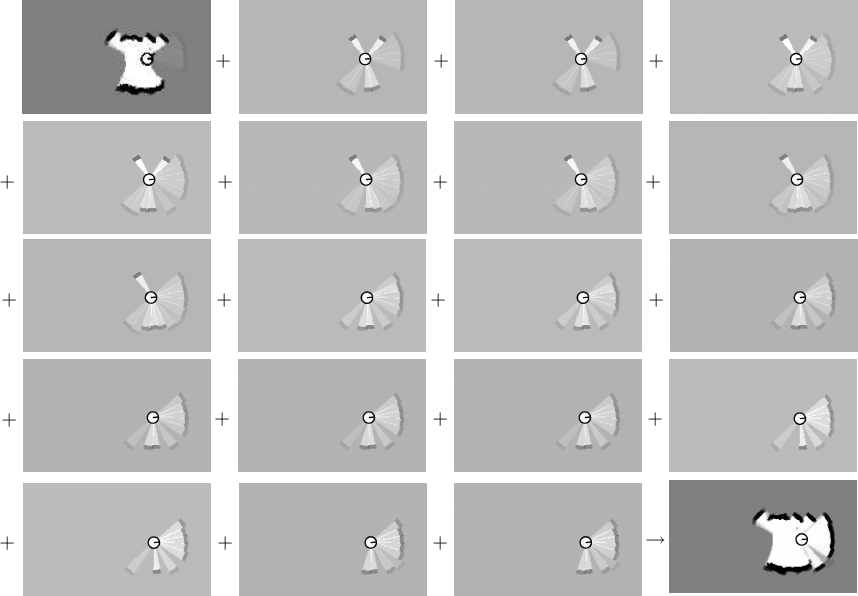
\includegraphics[width=0.95\linewidth]{imagenes/occgridUpdate.png}
  \caption[Aplicación de la regla de actualización propuesta en
  \cite{stachniss2009robotic} en un corredor.]{Aplicación de la
    regla de actualización propuesta en \cite{stachniss2009robotic} en un
    corredor. La imagen superior izquierda muestra el mapa inicial y
    la inferior derecha contiene el mapa resultante. Los mapas intermedios son los
    mapas locales construidos a partir de los sensores del robot. Extraída de
  \cite{stachniss2009robotic}. }
  \label{fig:mappingUpRule}
\end{figure} 



% Y por otro lado como estas actualizaciones se integra (el método que se describe en \cite{stachniss2009robotic}).
% notando que solo se considera los datos sensoriales
% aportados  el robot

% si
% esto genera un cambio en la grilla, este cambio se informa al modulo
% \emph{combinador de mapas}. 

% robot completa un objetivo de exploración este recopila nueva
% informacion del entorno a partir de sus sensores

% Comentar como funcina el map merger:

% las actualizaciones, que las da el stack de navegacion, lo que esto implica
% (los datos de los sensores se procesan en celdas), que son incrementales (solo
% porcion del mapa) tanto la entradas como las salidas



%%%%%%%%%%%%%%%%%%%%%%%%%%%%%%%%%%%%%%%%%%%%%%%%%%%%%%%%%%%%%%%%%%%%%%%%%%%%%%%%%%%%%%
% basura de planificación
% Resumiendo, la planificación jerarquica cosnsiste en utlizar el camino original
% para determinar los subobjetivos ubicados en las transicisiones entre los segmentos
% del camino y \emph{move base} para navegar dentro de los segmentos hacia dichas
% transiciones. 

% solo utilizar la información topologica contenida en
% los caminos originales generados sobre el GVD.

% (en su mayor parte compuesto por centros de celdas pertencientes a GVD) p
% que son más
% eficientes computacionalmente que los generados sobre todo el espacio libre de
% la grilla, sin las desventajas.
% no trivales se calcula sobre las celdas pertencientes al GVD, lo cual tiene
% menor costo computacional que considerar todo el espacio libre de la grilla de
% coupacion eficiente calcular.



% La ventaja de aplicar esta tecnica es que hace posible utlizar
% los caminos , 

% caminos sobre el GVD, pero los caminos resultantes pueden ser innecesariamente
% largos, mientras que \emph{move base} con la configuracion correcta, permite
% ejecutar de forma eficiente caminos cercanos a los lineales. De esta manera se
% aporvecha la eficiencia del calaculo de caminos sobre el GVD, y se evitan los
% desvios que dichos camnios tienen, solo utlizando de estos los subobjetivos que
% se ubican en portales, 


% del camino y \emph{move base} para navegar dentro de los segmentos hacia dichas
% transiciones. La ventaja de aplicar esta tecnica es que hace posible utlizar los camnios
% no trivales se calcula sobre las celdas pertencientes al GVD, lo cual tiene
% menor costo computacional que considerar todo el espacio libre de la grilla de
% coupacion eficiente calcular.


% Recordando que los caminos originales se contruyen principalmente sobre el GVD,
% los niveles de jerarquia son do

% Por e dado un valor de $\mli{DistNs}$ más grande que elPara ejemp esto  esto porque los subobjetivos
% para los cuales exite una línea  

%   \item Existe una línea recta de grosor minDesiredDistance que lo conectan con el
%     robot sin solaparse con ningun obstaculo y tampoco tienen obtaculos a minDesiredDistance. 
%   \item Esta a meno de una distancia Z (Z puede estar entre forcedCompletionTolerance y alcance de sensado)


% Lo que se suele obtener en entornos estructurados es que los robots se mueven
% libremente en el interior los segmentos, mientras que para pasar de segmento a
% segmento utiliza el gvd para pasar por los pasajes estrechos que consituyen las
% puertas.

% En el caso de un Y pequeño se tiene una navegacion que sigue de forma más estricta al GVD.



% Los objetivos triviales se definen como los objetivos para los cuales el
% segmento de recta que existe entre el robot y el objetivo no contiene
% obstaculos, de lo contrario el objetivo es no trivial. Para determniar esto, se
% discretiza el segmento de recta en celdas \cite{foleyphillips} y se comprueba
% en el mapa global (grilla de ocupacion) almacenado en el robot, alguna de las
% celdas tiene un estado ocupado.

% El camino en objetivos triviales se determina como dicho segmento de recta que
% existe entre el robot y el objetivo, que se encuentra libre de obstaculos. 




% Este camino se divide subobjetivos y objtivos. El
% objetivo es el objetivo asignado, ubicado al final del camino. Por otro lado
% subobjetivos, son puntos intermedios correspondientes a centros de celda

% planificar como llegar a dicho objetivo. 


% Luego de que la central concluye el proceso a traves del cual determina que
% objetivo asignar a un robot  e informa dicha
% asignacion.  

% asignado a un objetivo el robot deberá llegar hasta el, para esto es necesario
% solucionar el este problema de planificación. La solución desarrollada aplica
% las ideas de planificación jerárquica presentadas en la sección
% \ref{subsec:mapas}, con el motivo de permitir una planificación eficiente sin
% resultar en caminos innecesariamente largos.




% Referenciar los tipos de caminos a la parte de la valuacion que habla de esto.

% Describier el proceso a detalle desde que llega un camino, y como este se va
% completando poco a poco hasta llegar al objetivo de exploración al final del
% camino.

% Tocar por arriba los mecanismos de recuperacion si queda facil.

% \subsection{Subobjetivo}
% Es un punto intermedio de un camino que lleva a un objetivo, el cual debe ser percibido por los sensores del robot

% Un subobjetivo se considera completo si:
% \begin{itemize}
%   \item Existe una línea recta de grosor minDesiredDistance que lo conectan con
%     el robot sin solaparse con ningun obstaculo y tampoco tienen obtaculos a
%     minDesiredDistance. 
%   \item Esta a meno de una distancia Y (Y puede estar entre
%     forcedCompletionTolerance y $\infty$)
% \end{itemize}
% O si:
% \begin{itemize}
%   \item Esta a menos de una diatancia forcedCompletionTolerance (mencionada en otra seccion, se puede ver de reorganizar luego)
% \end{itemize}

% \subsection{Objetivo}
% Es el punto final de un camino, debe ser percibidopor los sensores del robot

% Un objetivo se considera completo si:
% \begin{itemize}
%   \item Existe una línea recta de grosor minDesiredDistance que lo conectan con el
%     robot sin solaparse con ningun obstaculo y tampoco tienen obtaculos a minDesiredDistance. 
%   \item Esta a meno de una distancia Z (Z puede estar entre forcedCompletionTolerance y alcance de sensado)
% \end{itemize}

% O si:
% \begin{itemize}
%   \item Esta a menos de una diatancia forcedCompletionTolerance (mencionada en otra seccion, se puede ver de reorganizar luego)
% \end{itemize}

% \subsection{Objetivos triviales}
% Estos objetivos son los que tienen una línea recta de grosor X que lo conectan
% con el robot sin solaparse con ningun obstaculo y tampoco tienen obtaculos a
% X. X puede ser el maximo tamaño de una puerta o la minDesiredDistance.
% \begin{itemize}
%   \item Yo use un estimado del max tamaño de la puerta para evitar objetivos
%     triviales  que esten en un segmento distinto del que esta el robot
% \end{itemize}

% Estos objetivos tienen el trato especial de que los camninos planificados a
% estos no son sobre el GVD si no que consiten solo en el objetivo trivial.

% Esto facilita la navegacion cuando el camino al objetivo es muy facil, es decir es trivial.

% \subsection{Objetivos no triviales}

% Cuando el objetivo no es trivial lo que se hace es obtener un camnino utilizando el
% gvd como roadmap.

% Cada punto de este camnio es un subobjetivo menos el ultimo que es el objetivo
% en si. El robot siempre se dirige al ultimo subobjetivo/objetivo no competado.

% De esta forma notando las condiciones de complecion si Y es grande se tiene 
% navegacion libre (delegada a move base, el nivel bajo de la jerarquia) sobre
% zonas para las cuales no existen obtaculos mientras que se navega siguientdo el
% camnino seguro (provisto por el gvd, nivel alto de la jerarquia) cuando los
% objetivos son \say{no deseables} o \say{no seguros}.

% Lo que se suele obtener en entornos estructurados es que los robots se mueven
% libremente en el interior los segmentos, mientras que para pasar de segmento a
% segmento utiliza el gvd para pasar por los pasajes estrechos que consituyen las
% puertas.

% En el caso de un Y pequeño se tiene una navegacion que sigue de forma más estricta al GVD.

% % Entiendo que Y grande es mejor:
% %   `Una prueba para validar esto sería probar: Y en [50,10,5 2.5]`

% \subsection{Recupaeracion}

% \begin{itemize}
% \item Primero: "si tengo un objetivo activo y no estoy avanzando a el entoces intento recuperarme"
%   \begin{itemize}
%   \item Para saber el objetivo actual interceptar el next.
   
%   \item Si el objetivo cambia                           $=>$ reiniciar tiempo y distancia del ultimo avance.

%   \item Si la distancia es menor a la del ultimo avance $=>$ actualizar tiempo y distancia del ultimo avance

%   \item Si pasan X segundo desde el ultimo avance y el camino no esta completo =>
%     \begin{itemize}
%     \item Hacer recovery
%     \item reiniciar el timepo desde el ultimo avance (dejar un rato antes del proximo recovery)
%     \end{itemize}
%   \end{itemize}

% \item Segundo: "Si segun yo lo complete pero la central me dice que no esta completado seguramente no lo estoy viendo correctamente, intento recuperarme"
%   \begin{itemize}
%   \item Si se reasigna al objetivo => Hacer recovery
%   \end{itemize}
% \end{itemize}

% La recuperacion cosiste de:
% \begin{itemize}
%   \item  ir un poco para atras (en direccion opuesta al objetivo)
%   \item  esperar un tiempo estimando la llegada a la posicion a la que se fue en el punto anterior
%   \item  notificar a la central de la recuperacion para reasisgnar objetivos:
%   \begin{itemize}
%     \item Util por cambiar la pos del robot tanto en Primero como en Segundo
%     \item Util en segundo porque capaz ahora si se completo el objetivo
%   \end{itemize}
%   \item  Mientras la central no atienda al pedido volver al objetivo y eventualmente seguir con el camino
% \end{itemize}

%%%%%%%%%%%%%%%%%%%%%%%%%%%%%%%%%%%%%%%%%%%%%%%%%%%%%%%%%%%%%%%%%%%%%%%%%%%%%%%%%%%%%
% basura de GVD
% Dado esto se puede afirmar que $c_1$ y $c_2$ pertenecen al GVD si y solo si
% $oc_1\neq oc_2$ y no son adyacentes, 

% Hablar de la necesidad de encontrar las celdas base para lograr definir la
% líneas criticas y posteriormente lograr segmentar (seccion \ref{subsec:mapaTopGVDGrid}).

% Mencionar la solucion a la que se llego, y cual es la definicion de celda base.
% Dos caminos (I) mi definicion que separa los basis en sources y pseudosources. O (II)
% definir los basis como las celdas ocupadas que hacen que una celda pertenezca
% al GVD segun lau (solo se neceita para puntos criticos incluidos en el GVD). 

% (II) tiene la ventaja que es facil de explicar y permite basarse en lo que ya
% esta bien fundamnetado (Lau), por otro lado (I) es lo que se implemento, pero
% puede ser dificil de explicar, sin tener mucho fundamento más que el
% generalizar y definir bien para el haberlo hecho asi. (puedo tomarme un tiempo
% para pensar en algun acaso claro y facil de epxlicar donde (I) esto funcione
% mejor pero no se)

% (I) aplica el criterio de siegwart-ming que capaz esta bueno que sea epxlicito.

% (I) permite comentar el tema de dist 1. (se puede mencionar en II tambien,
% diciendo que se hace eso pero que en realidad se saco si experimetnar el rido
% que dice que evita)

% Se puede intentar comentar todo en alto nivel

%%%%%%%%%%%%%

% Comentar como a partir de esta definicion de celda base, y las nociones de no
% adyacentes ni iguales entoces diferentes generadores (parrafo más abajo) se
% logra una nueva condicion de pertenencia al GVD, la cual esta más cercana a la
% definicion de GVD en el espacio continuo. (aunque aca cuidado, que tan distinta
% es al final? no se hace algo similar pero solo usando el obstaculo más
% cercano?) capaz puedo ir por ese lado y siendo más facil basarse en el trabajo
% de lau que redefinir sin mucho fundamento.

% Bueno hay una diferencias, la condicion de distancias de liu ming, y que no se
% permiten pseudosources adyacentes entre si. Ademas que se mantiene un registro
% de pseudosources.

% Son detalles que estan buenos para mi, porque son más generales mejor definidos
% pero no se que tanto puedo fundamentar su necesidad, y por lo tanto no se que
% tanto aporta dar toda la epxlicacion para lo que cuesta explicar y entender, creo que se
% puede epxlicar más facilmente con un solo obstaculo y esableciendo los oc que
% hicieron que pertenezca al GVD.

% fue necesario analizar el
% funcionamiento del algorimo.

% Hablar de que en \emph{brushfire dinamico} no se manejan los generadores de forma directa,

% Dado esto, 
% se decidio definir los puntos que base discretizados $\mli{BPD}_c$ 
% como las celdas obstaculizadas no adyacentes que generan la pertenecia
% de una celda $c$ al GVD.
% Establecido esto, es pertinente notar que la implementacion de \emph{brushfire
% dinamico} hecha en este proyecto difiere en la original en que esta almacena
% las celdas ocupadas que generan la pertenecia de un punto al GVD para ser
% utilizados posteriormente como puntos base.


% A lo largo de esta seccion se explicaran las conicidencia y cambios entre
% \emph{brushfire dinamico} y la variante de este implementada en este proyecto.

% \subsection{Algorimo general}

% \begin{algorithm}[H]
% \SetAlgoLined
% \SetKwProg{Fn}{Function}{}{}

% \Fn{establecerFuente(f)}{
%   $F_i := {f}$\\ 
%   $\mli{PF}_i := \emptyset$\\
%   $\mli{DD} := 0$\\
%   $removido := falso$
% }


% \Fn{removerObstaculo(oc)}{
%   $F_i := \emptyset$\\ 
%   $\mli{PF}_i := \emptyset$\\
%   $\mli{DD} := \infty$\\
%   $removido := verdadero$
% }
    
% \caption{Brushfire }
% \label{alg:DinBF}
% \end{algorithm}
% poner pseudocodigo de todo lo que hice basado en el de lau
% Si se sigue entendiendo lo de abajo sin esto me parece mejor evitarlo (muy similar a lau que ya se explico (sin pseudo pero la idea si) y la explicacion ocn pseudo puede llevar algunas carillas)

% \subsection{Pertenecia}
% La implemetacion realizada en proyecto mantiene las olas conistentes e
% inconsistentes para el calulo incremental de mapas de distancia. Tambien
% mantiene la idea que las olas inconsistentes remueven las celdas que atraviesan
% del GVD y la idea de que las celdas en las cuales las ondas consistentes se
% detienen y las celdas que causaron que se detengan son las celdas cuya
% pertenencia al GVD se comprueba.

% capaz prodria decir la def de pertenecia dado un choque de olas, explicar que
% un choque de olas siempre se da entre dos celdas, explicar el de lau, y el mio,
% estableciendo bien como es el tema de los pseudosources y las diff, dada la
% info que lleva la ola, etc. Aunque puede ser dificil dar ejemplos

% El cambio que se hace es en el criterio con el cual se comprueba la pertenencia
% de una celda. En el \emph{brushfire dinamico} original se hace EXPLICAR
% CON LO DE más ABAJO. En esta implementacion cambia, al existir un choque de
% olas primero se establecen los pseudosources y luego de existir dos
% pseudosources no adjacentes entre si la celda pertenece.

% Explicar definicion de un pseudosource (SACAR DE LAS NOTAS), y porque esto termina siendo distinto
% que lo que se plantea en el \emph{brushfire dinamico} original.

% Capaz que explicar que el evitar generar si no hay dos basis no vecions es el evitar generar incorrectamente gvd en corredores diagonales. (aunque puede dar lugar a la discucion de que pasa si no es completamente diagonal, cosa que sospecho que puede dar problemas similares)

% Oportunidad de comentar que mejora sobre lau porque perminte generar gvd en
% lugares a dist 1 (ver bien que), cosa que lau no permite por resistencia al ruido pero que con el método actual no llevo mayores inconvenientes permitiendo generar gvd en grillas con el maximo tamaño de celda posible en el cual las puertas más chicas consisten de una unica celda ejemplo de algo asi: (esta en comentarios de latex)

%   mio            lau
% - - | - -      - - - - -
% - - | - -      - - - - -
% X X | X X  VS  X X - X X 
% - - | - -      - - - - -
% - - | - -      - - - - -

% Explicar que quizas se relacione al tema corredor de largo 2 que se va a explicar en \ref{subsec:filt}.

% \subsection{Filtrado}\label{subsec:filt}
% Los vetices que en una iteracion se determina que deben pertenecer al GVD segun
% el criterio de pertenecia aplicado en las celdas en las cuales se detiene una
% ola consistente, pasan por un filtrado extra. Este filtrado busca evitar líneas
% discretizadas de dos celdas de grosor que violan la propiedad \say{sparceness}
% GVD.

% As discussed before, different paths on the Voronoi graph correspond to
% topologically different routes in the environment (sparceness property). To preserve this property
% for GVDs on grid maps, thin Voronoi lines, i.e., being one pixel wide, are
% desired.

% Spacrceness:Their application as roadmaps is an appealing technique for path
% planning, since they are “sparse” in the sense that different paths on the
% graph correspond to topologically different routes with respect to obstacles.
% This

% En el \emph{brushfire dinamico} original el filtrado se lleva a cabo haciendo
% uso de patrones con los cuales se comprueba si el GVD queda o no disconexo

% Our optional pruning step erodes 2-pixel-wide Voronoi lines. Therefore, all
% new Voronoi cells are inserted into a priority queue and processed by the
% pruning stage. The image operator patterns shown in Fig. 6 (solo poner
% 8-connected) match whenever the center cell s provides connectivity for one or
% more of its adjacent cells. In any pattern, a $1$ matches voro(s) = true, while
% $0$ stands for voro(s) = false, and empty fields are ignored. Where indicated
% by arrows, the same pattern is applied in all unique 90 degree rotations

% The second phase implements the actual pruning step. In increasing order of
% distance, the enqueued cells are iteratively popped from the priority queue. If
% such a cell has more than one neighbor on the GVD and is not required to keep
% the GVD connected, it can be removed from the GVD without affecting its
% topology. Again, this is tested using the image operator patterns: if none of
% the connectivity patterns match at the cell location, the cell is not required
% in the GVD.

% Enfasis en $P^8_1$ que indica que las celdas con un solo vecino deben pertenecer al GVD.

% En el caso de la implementacion del proyecto se comprueba si el GVD queda
% disconexo aplicando la tecnica presente en \cite{zhang1984fast},
% adicionalmente evitando filtrar celdas con una sola celda adyacente en el GVD
% y con 2 celdas ayacentes en el GVD si estas se detectan en un corredor.

% Explicar caso corredor(SACAR DE LAS NOTAS). comentar que no se considera en
% lau, quizas este es un problema que se arregla no permitiendo dist = 1. Aunque
% más analisis son necesarios

% \subsection{Limpieza de aristas}
% La limpieza de aristas es una tecnica aplicada solo en la implementación del
% proyecto esta permite generar GVD más limpios. 


% \subsection{Segmentacion}
% yo diria de 

% Creo que aca en realidad no habria que comentar mucho si es que hay que comentar, son las mismasideas que las comentadas en \ref{subsec:mapaTopGVD}.

% Quizas mencionar que se usa la descomposición en componentes conexas y como. 

% Mencionar el uso de sources y pseudosources para hacer líneas criticas. Discretizacion de líneas?

% Algunos resultados?

%%%%%%%%%%%%%%%%%%%%%%%%%%%%%%%%%%%%%%%%%%%%%%%%%%%%%%%%%%%%5

% basura de: \subsection{simplificación de fronteras basada en cubrimiento}

 %  \item Actualizar $\mli{FS_i}$ agregando $\mli{fs}$:

 %    $\mli{FS_i} := \mli{FS_i} \cup \{\mli{fs}\}$

 %  \item Actualizar $\mli{UF}$ removiendo todas las fronteras cubiertas por $\mli{fs}$:

 %    $\mli{UF} := \mli{UF} - \mli{RC}$

 %    Con $\mli{RC}=\{ f\in F_i : d_{\mli{fs}}(f) \leq rango\}$ las celdas recien
 %    cubiertas.

 %  \item Si $\mli{UF} \neq \emptyset$ volver a 1. de lo contrario devolver $FS_i$.
% \end{enumerate}



% Adicionalmente, se simepre que sea menor a $rango$ se usara la heuristica de 



% eleccion de
% $\mli{fs}$ debe considerar el resto de fronteras por cubrir y su cercania a los
% obtaculos, por ejemplo si $\mli{UF}$ es tan pequeño como para que se cubra
% completamente con una unica frontera significativa $\mli{fs}$ esta se deberia
% elegir para que este centrada en $\mli{UF}$.
%%acatoy
% Se asume que las fornteras más centradas se encuentran a una
% distancia $dCen = max\{ d_{\mli{PF}}(\mli{f}) : f\in\mli{UF} \}/2$ de
% $\mli{pf}$. 

% Combiando ambos factores se determina que el conjunto de fronteras
% significativas candidatas 

 % puede resumir como elegir una frontera $\mli{fs}$ que
% cubra 

% comienza desencolando una frontera $\mli{pf}$ de $\mli{PF}$
% que debe no estar cubierta todavia, por lo cual de estar cubierta se descarta y
% se vuelve a desencolar. 


% , si dicha forntera ya esta cubierta la eleccion se cancela 
% \begin{enumerate}
 %  \item 
 %  \item Actualizar $\mli{FS_i}$ agregando $\mli{fs}$:

 %    $\mli{FS_i} := \mli{FS_i} \cup \{\mli{fs}\}$

 %  \item Actualizar $\mli{UF}$ removiendo todas las fronteras cubiertas por $\mli{fs}$:

 %    $\mli{UF} := \mli{UF} - \mli{RC}$

 %    Con $\mli{RC}=\{ f\in F_i : d_{\mli{fs}}(f) \leq rango\}$ las celdas recien
 %    cubiertas.

 %  \item Si $\mli{UF} \neq \emptyset$ volver a 1. de lo contrario devolver $FS_i$.
% \end{enumerate}

%%%%%%%%%%%%%%%%%%%%%%%%%%%%%%%%%%%%%%%%%%%%%%%%%%%%%%%%%%%%%%%%%%%%%%%%%%%%%%%%%%%%%

% De los pasos presentados el primero es el principal y tambien el más complejo
% del algorimo.

% Los pasos del 2 al 4 no presentan ambigüedad, siendo el paso 1 en el que resta
% aclarar, especificamente lo que resta aclarar es el criterio con el que se
% elige la frontera significativa. La eleccion en un principio podria ser
% aleatoria y el algoritmo daria resultados validos, pero esto dejaria a la
% suerte la calidad de la solucion. La idea sería elegir de forma determinista a
% una frontera significativa buscando que cubra la mayor cantidad de frotneras
% mientras se evita cubrir nuevamente fronteras que ya sean cubiertas por otra
% frotntera significativa. 

% La tecnica desarrollada se basa en mantener una cola FIFO en donde se guardaran
% los proximas fronteras a cubrir $\mli{PF}$, 
% El proceso para elegir una nueva forntera significativa $\mli{fs}$ consiste en
% desencolar una frontera $\mli{PF}$ de $\mli{PF}$ para posteriomente determinar
% el conjunto de fronteras significativas candidatas $\mli{FSC}$ como las
% fronteras sin cubrir desde las cuales se cubre a $\mli{PF}$ estando lo más
% alejadas posible de esta, es decir, que $\mli{FSC}$ %$= \{f\in \mli{UF} : d_{\mli{fs}}(\mli{PF})= rango$\}
% sera el conjunto de celdas en $\mli{UF}$ que solapen con la circunferencia del
% circulo de radio $rango$ centrada en $\mli{PF}$ denotada como $\mathscr{C}(\mli{PF},rango)$.
% Para elegir una nueva frontera significativa $\mli{fs}$ se debe elegir una
% frontera de $\mli{FSC}$, que en esta propuesta se hace de forma arbitraria.


% Ahora resta tratar dos casos bordes, el primero es la inicializacion de
% $\mli{PF}$ cuando no existen fronteras adyacentes a obstaculos, cuando esto
% sucede para inciar el algorimo basta con agregar una unica frontera arbitraria
% de $F_i$ a $\mli{PF}$. El otro caso es el que se presenta si $\mli{FSC} = \emptyset$
% \todo{esto esta mal, en realidad esta mal desde antes cuando se presenta FSC, FSC busca que las candidatas queden centradas. Por lo que el radio puede ser menor al rango aunque haya una (o más) celda solapada conla circunferencia de radio rango}
% , es
% decir la circunferencia del circulo de radio $rango$ centrada en $\mli{PF}$ no
% se solapa con ninguna celdas en $\mli{UF}$. Cuando esto sucede lo que se hace
% es reducir el radio del circulo a $\frac{max\{ d_{\mli{PF}}(\mli{f}) :
% f\in\mli{UF} \}}{2}$ la divicion entre dos busca que la circunferencia se
% solape sobre el punto medio entre $\mli{PF}$  y la celda de $\mli{UF}$ más
% alejada de $\mli{PF}$, quedando la nueva frontera significativa centrada
% (figura ejemplo de esto).

% Para que el criterio de eleccion propuesto funcione de forma correcta es
% necesario agregar al paso 2 que  se deben encolar a $\mli{PF}$ todas las
% fronteras del siguiente conjunto $\{ f \in \mli{UF} : \exists c \in \mli{FS_i}
% - \mli{UF}, f \in ady(c)\}$ que no esten ya encoladas.

% $\mil{CF}$ de las fronteras
% cubiertas pos la nueva $\mli{fs}$, encolan a $\mil{PF}$ a las celdas de $


% elegir
% $\mli{fs}$ como uno de las 

% La condicion de distancia busca maximizar la
% cantidad de fronteras que cubre la nueva frontera significativa.

% EL algorimo se basa en la idea de que una buena distribucion de fronteras
% significativas deberia mantener en su mayor parte una distancia de $rango*2$
% entre cada frontera significativa, ya que esta es la distancia maxima que se
% puede tener para asegurar qu se cumpla el cubrimiento. 
